%%%%%%%%%%%%%%%%%%%%%%%%%%%%%%%%%%%%%%%%%
% Daily Laboratory Book
% LaTeX Template
% Version 1.0 (4/4/12)
%
% This template has been downloaded from:
% http://www.LaTeXTemplates.com
%
% Original author:
% Frank Kuster (http://www.ctan.org/tex-archive/macros/latex/contrib/labbook/)
%
% Important note:
% This template requires the labbook.cls file to be in the same directory as the
% .tex file. The labbook.cls file provides the necessary structure to create the
% lab book.
%
% The \lipsum[#] commands throughout this template generate dummy text
% to fill the template out. These commands should all be removed when 
% writing lab book content.
%
% HOW TO USE THIS TEMPLATE 
% Each day in the lab consists of three main things:
%
% 1. LABDAY: The first thing to put is the \labday{} command with a date in 
% curly brackets, this will make a new page and put the date in big letters 
% at the top.
%
% 2. EXPERIMENT: Next you need to specify what experiment(s) you are 
% working on with an \experiment{} command with the experiment shorthand 
% in the curly brackets. The experiment shorthand is defined in the 
% 'DEFINITION OF EXPERIMENTS' section below, this means you can 
% say \experiment{pcr} and the actual text written to the PDF will be what 
% you set the 'pcr' experiment to be. If the experiment is a one off, you can 
% just write it in the bracket without creating a shorthand. Note: if you don't 
% want to have an experiment, just leave this out and it won't be printed.
%
% 3. CONTENT: Following the experiment is the content, i.e. what progress 
% you made on the experiment that day.
%
%%%%%%%%%%%%%%%%%%%%%%%%%%%%%%%%%%%%%%%%%

%----------------------------------------------------------------------------------------
%	PACKAGES AND OTHER DOCUMENT CONFIGURATIONS
%----------------------------------------------------------------------------------------

\documentclass[idxtotoc,hyperref,openany]{labbook} % 'openany' here removes the gap page between days, erase it to restore this gap; 'oneside' can also be added to remove the shift that odd pages have to the right for easier reading

\usepackage[ 
  backref=page,
  pdfpagelabels=true,
  plainpages=false,
  colorlinks=true,
  bookmarks=true,
  pdfview=FitB]{hyperref} % Required for the hyperlinks within the PDF
  
\usepackage{booktabs} % Required for the top and bottom rules in the table
\usepackage{float} % Required for specifying the exact location of a figure or table
\usepackage{graphicx} % Required for including images2
\usepackage{lipsum} % Used for inserting dummy 'Lorem ipsum' text into the template
\usepackage[shortlabels]{enumitem}
\usepackage{pgfplots, pgfplotstable}
\usepackage{siunitx}

\newcommand{\HRule}{\rule{\linewidth}{0.5mm}} % Command to make the lines in the title page
\setlength\parindent{0pt} % Removes all indentation from paragraphs

%----------------------------------------------------------------------------------------
%	DEFINITION OF EXPERIMENTS
%----------------------------------------------------------------------------------------

\newexperiment{example}{This is an example experiment}
\newexperiment{example2}{This is another example experiment}
\newexperiment{example3}{This is yet another example experiment}
\newexperiment{table}{This shows a sample table}
%\newexperiment{shorthand}{Description of the experiment}

%---------------------------------------------------------------------------------------

\begin{document}

%----------------------------------------------------------------------------------------
%	TITLE PAGE
%----------------------------------------------------------------------------------------

\frontmatter % Use Roman numerals for page numbers
\title{
\begin{center}
\HRule \\[0.4cm]
{\Huge \bfseries Laboratory Journal \\[0.5cm] \Large Bachelor of Science}\\[0.4cm] % Degree
\HRule \\[1.5cm]
\end{center}
}
\author{\Huge Tiffany Pham \\ \\ \LARGE tpham118@ucmerced.edu \\[2cm]} % Your name and email address
\date{Beginning 24 January 2024} % Beginning date
\maketitle

\tableofcontents

\mainmatter % Use Arabic numerals for page numbers

%----------------------------------------------------------------------------------------
%	LAB BOOK CONTENTS
%----------------------------------------------------------------------------------------

% Blank template to use for new days:

%\labday{Day, Date Month Year}

%\experiment{}

%Text

%-----------------------------------------

%\experiment{}

%Text

%----------------------------------------------------------------------------------------

\labday{Wednesday, 24 January 2024}

\experiment{Lab Notebook Prompts}
\begin{enumerate}
    \item Maintaining Your Laboratory Notebook: This course specifies how to maintain and organize information in your lab notebook, which will help you develop this important research skill. Figures 1 – 8 are examples of various lab notebooks from undergraduates, graduate students, professors, and famous scientists in history.
    \begin{enumerate}[(a)] % (a), (b), (c), ...
        \item Which of the examples have characteristics that match the Maintaining Your Laboratory Notebook from the guide? Give the figure number and details of what matches.
    \end{enumerate}
    \item Notebook sections: The examples are just 1-2 pages from long-term research efforts; in practice, scientists develop their own style of keeping a lab notebook. Match each example with the applicable notebook section we’re having you use. Explain your choice.
    \item Reproducibility is important in science. Assuming the examples are typical of how the researcher keeps their lab notebook, which of the examples written in English would be easiest to use for repeating the experiment? Most difficult? Explain.
    \item Explain the value of not deleting or erasing mistakes, errors, or misunderstandings from your lab notebook. Why do we specify that you will need to identify and mark the error, explain how you identified that it was an error, and detail how you corrected it?
    \item Plan for your own notebook.
    \begin{enumerate}[(a)]
        \item What aspects of keeping a lab notebook do you expect to do well throughout the semester? Explain, referencing the rubric.
        \item Some aspects will need more practice. In what areas will TA feedback be most helpful as they grade your lab notebooks?
        \item What questions, if any, do you have about the lab notebook guide and rubric?
    \end{enumerate}
    \item Create a single, multi-page PDF of your answers. If your responses are all on one page, please draw a picture and add a funny comic (keep it safe for work!) on a second page. This is to ensure you know how to create multi-page PDFs. There are instructions above for how to create a PDF if you wrote things up on paper or PDF if you used OneNote without awkwardly cutting off lines or images. \textbf{It is your responsibility to ensure that your PDF is legible and uploaded correctly.}
\end{enumerate}

%-----------------------------------------

\experiment{Lab Notebook Answers} % Multiple experiments can be included in a single day, this allows you to segment what was done each day into separate categories
\begin{enumerate}
    \item Figure 2 is an excellent example of a lab notebook as they include a header and date and even have time slots for what they did during those times. They also included their goals for the week. and their objectives. Plus, their handwriting is neat and legible.
    \item Notebook Sections:
    \begin{enumerate}[(a)]
        \item \textbf{Figure 1:} Fits with the \textbf{handwriting section}; their handwriting is not messy as it is neat and legible.
        \item \textbf{Figure 2:} Fits with the \textbf{page headers section}; they wrote the date, title, and the names of all participants involved in the experiment.
        \item \textbf{Figure 3:} Fits with the \textbf{annotations section}; they used marks on the margins of the paper to bring attention to certain points. They also underlined and drew diagrams to help their notes.
        \item \textbf{Figure 4:} Fits with the \textbf{annotations section}; they underlined the important parts of their notes and also included a model drawing of their experiment.
        \item \textbf{Figure 5:} Fits with the \textbf{date and page numbers section}; they wrote the page number on the top corner of their page.
        \item \textbf{Figure 6:} Fits with the \textbf{title section}; they included the title and objectives of their experiment for that day.
        \item \textbf{Figure 7:} Fits with the \textbf{mistakes section}; they crossed out some of what they wrote but did not erase it. So they showed their mistakes and just continued on after
        \item \textbf{Figure 8:} Fits with the \textbf{mistakes section}; They wrote all their calculations down but didn't erase their mistakes. You can see some calculations that are crossed out.
    \end{enumerate}
    \item Figure 3 would be best to reproduce as they list the steps for what they did clearly, and the handwriting is neat and legible.
    \item It is important not to erase any mistakes, errors, or misunderstandings from your lab notebook as they are fundamental to the scientific process. In scientific research, identifying and correcting errors in a lab notebook are integral processes to uphold transparency, reliability, and the advancement of knowledge. Usually, identifying errors will involve meticulously reviewing experimental data, cross-checking with established protocols, collaborative discussions, and comparison with controls. The documentation of error identification includes clear annotations, contextual information, and an analysis of the circumstances surrounding the mistake. Detailing the correction process requires a step-by-step account of the actions taken, presentation of corrected data alongside original records, and a reflection on lessons learned. By doing this, it emphasizes collaboration, acknowledging team contributions, and discussing preventive measures that will enhance the overall integrity of the scientific process. This comprehensive approach ensures accurate and reproducible results and fosters a culture of continuous improvement and accountability within the scientific community.
    \item Planning Notebook:
    \begin{enumerate}[(a)]
        \item Based on what is written on the rubric, I think I could keep up my general notebook maintenance, such as writing down the date, page numbers, page headers, lab titles, etc. Usually, the upkeep is pretty easy, and because my lab notebook is online, it is easy to adjust and edit the format. I think I would also do well on the objectives, purpose, and prediction criteria. Usually, the objectives, purpose, and prediction criteria are some of the first things you write down, and you usually copy and paste these down, so these are pretty straightforward and easy. Another part of the rubric I think I could do well on is the experimental plan/ procedure, as some are also already known, and some are copied, pasted, and straightforward. Then, anything else below those criteria, I could do, but I probably won't be able to complete them 100\% or perfectly.
        \item In my opinion, I think I would get the most out when the feedback I get is on my data; data analysis and interpretations and also my lab reflections.
        \item I have no questions.
    \end{enumerate}
\end{enumerate}

%----------------------------------------------------------------------------------------

\labday{Wednesday, 31 January 2024}
\vspace{-5mm}
Tiffany Pham

\experiment{Lab 02 (Lab) - Is Your Phone a Good Protractor?}
\vspace{-5mm}
\textbf{Purpose}

This lab serves three purposes. 1) Become familiar with lab equipment. 2) Gain experience
collecting and analyzing real data and making reasoned, supported conclusions on what that data
means. 3) Practice recording what you’re doing and why in your lab notebook.

\hfill \break
\textbf{Predictions}

I predict that the protractor and phone will have similar values to each other with only an offset of +-10 degrees.

\hfill \break
\textbf{Procedure}

Walk around each of the tables (no particular order) and place phone perpendicular to the track. Record the data for the phone, then measure with the protractor and record data for protractor. Repeat for all tracks till you have data set filled out.

\hfill \break 
What could go wrong:

Phone cameras messing up measuring, can place phone camera off the track

Place perpendicular so phone cameras don't mess up (depending on the phone and case).

\hfill \break
\textbf{Equipment needed}

Phyphox downloaded on phone

Protractor

Track


%----------------------------------------------------------------------------------------

\experiment{Phone Measurements}

\begin{figure}[H] % Example of including images
\begin{center}
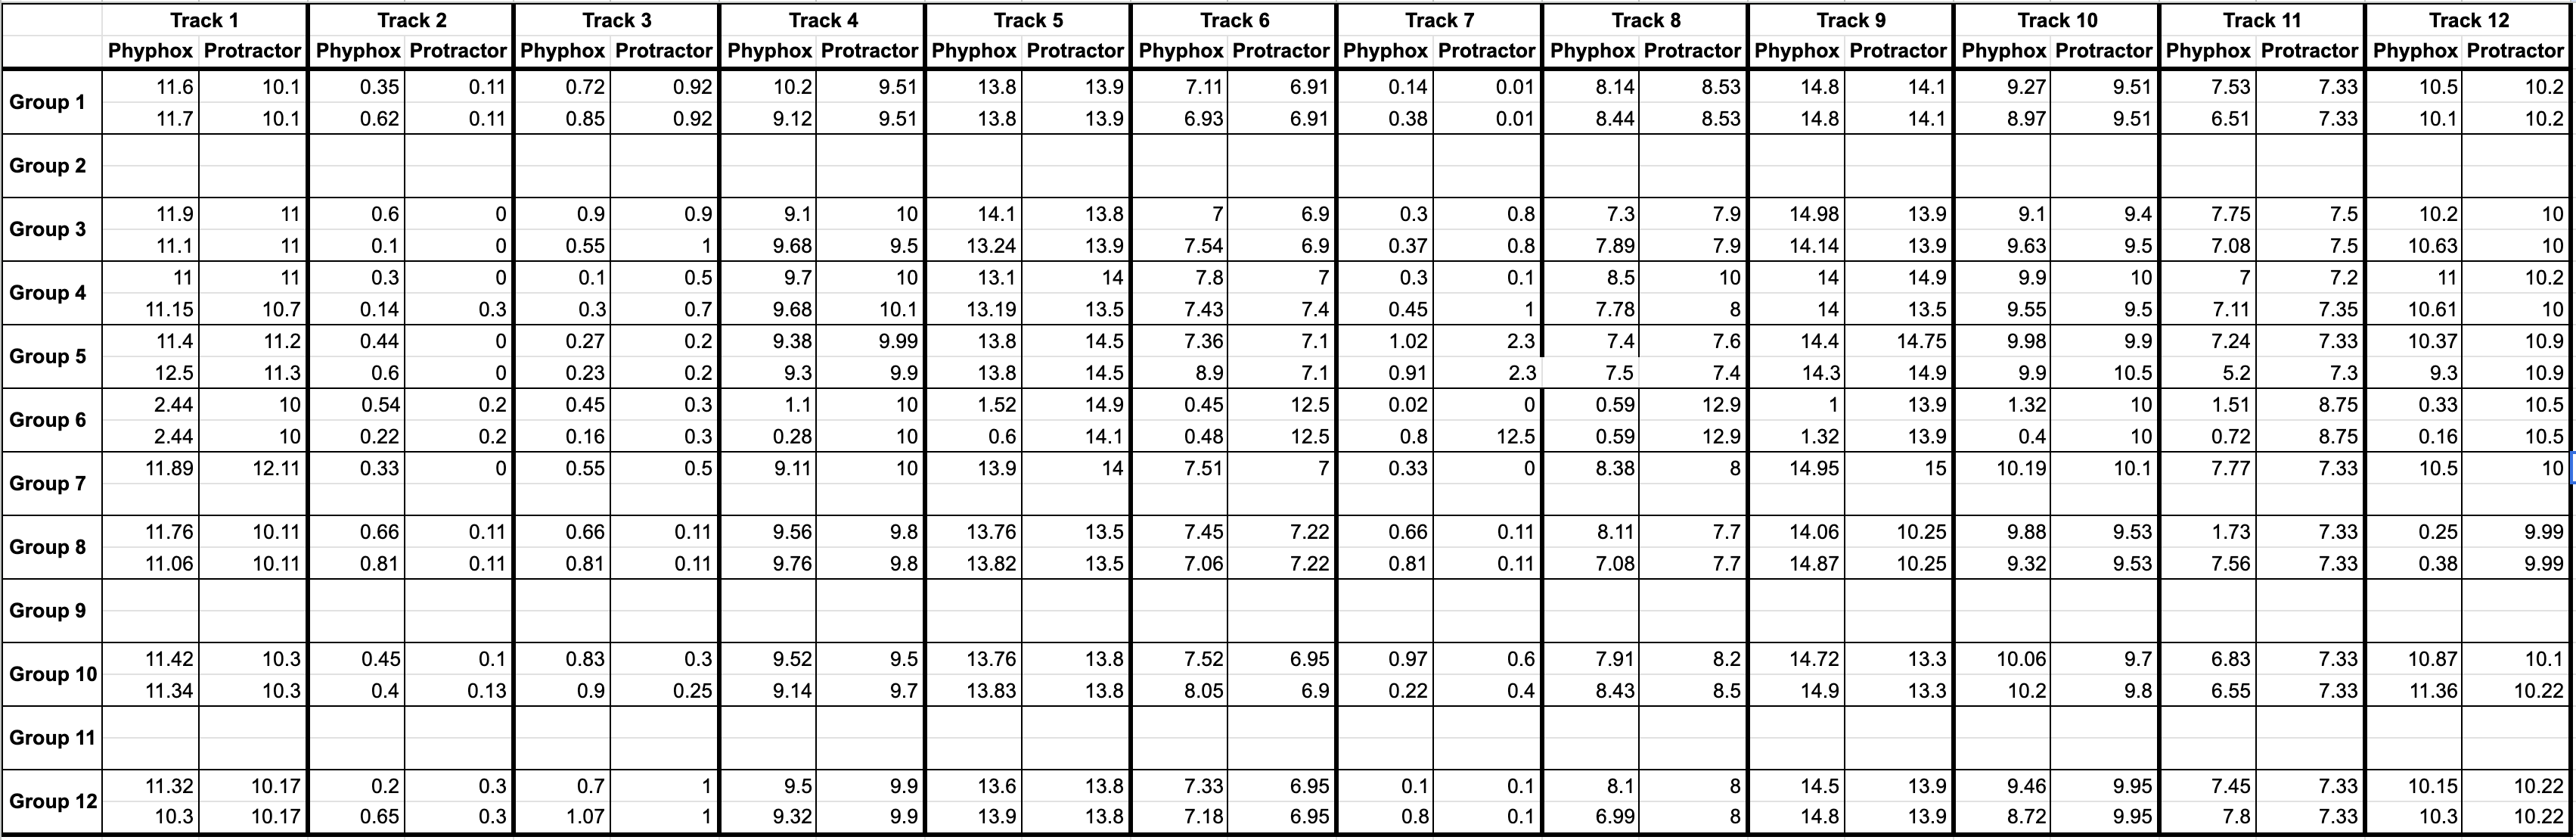
\includegraphics[width=1.25\linewidth]{images/Lab.01/PhyphoxProtractorSpreadsheet.png}
\end{center}
\caption{Data of Phyphox and Protractor Measurements}
\label{fig:Data of Phyphox and Protractor Measurements}
\end{figure}

Figure \ref{fig:Data of Phyphox and Protractor Measurements} shows all data collected from all groups for both the Phyphox app and the Protractor.

\hfill \break
\vspace{3in}
\hfill \break
\experiment{Calculating}
\hfill \break
\begin{figure}[H] % Example of including images
\begin{center}
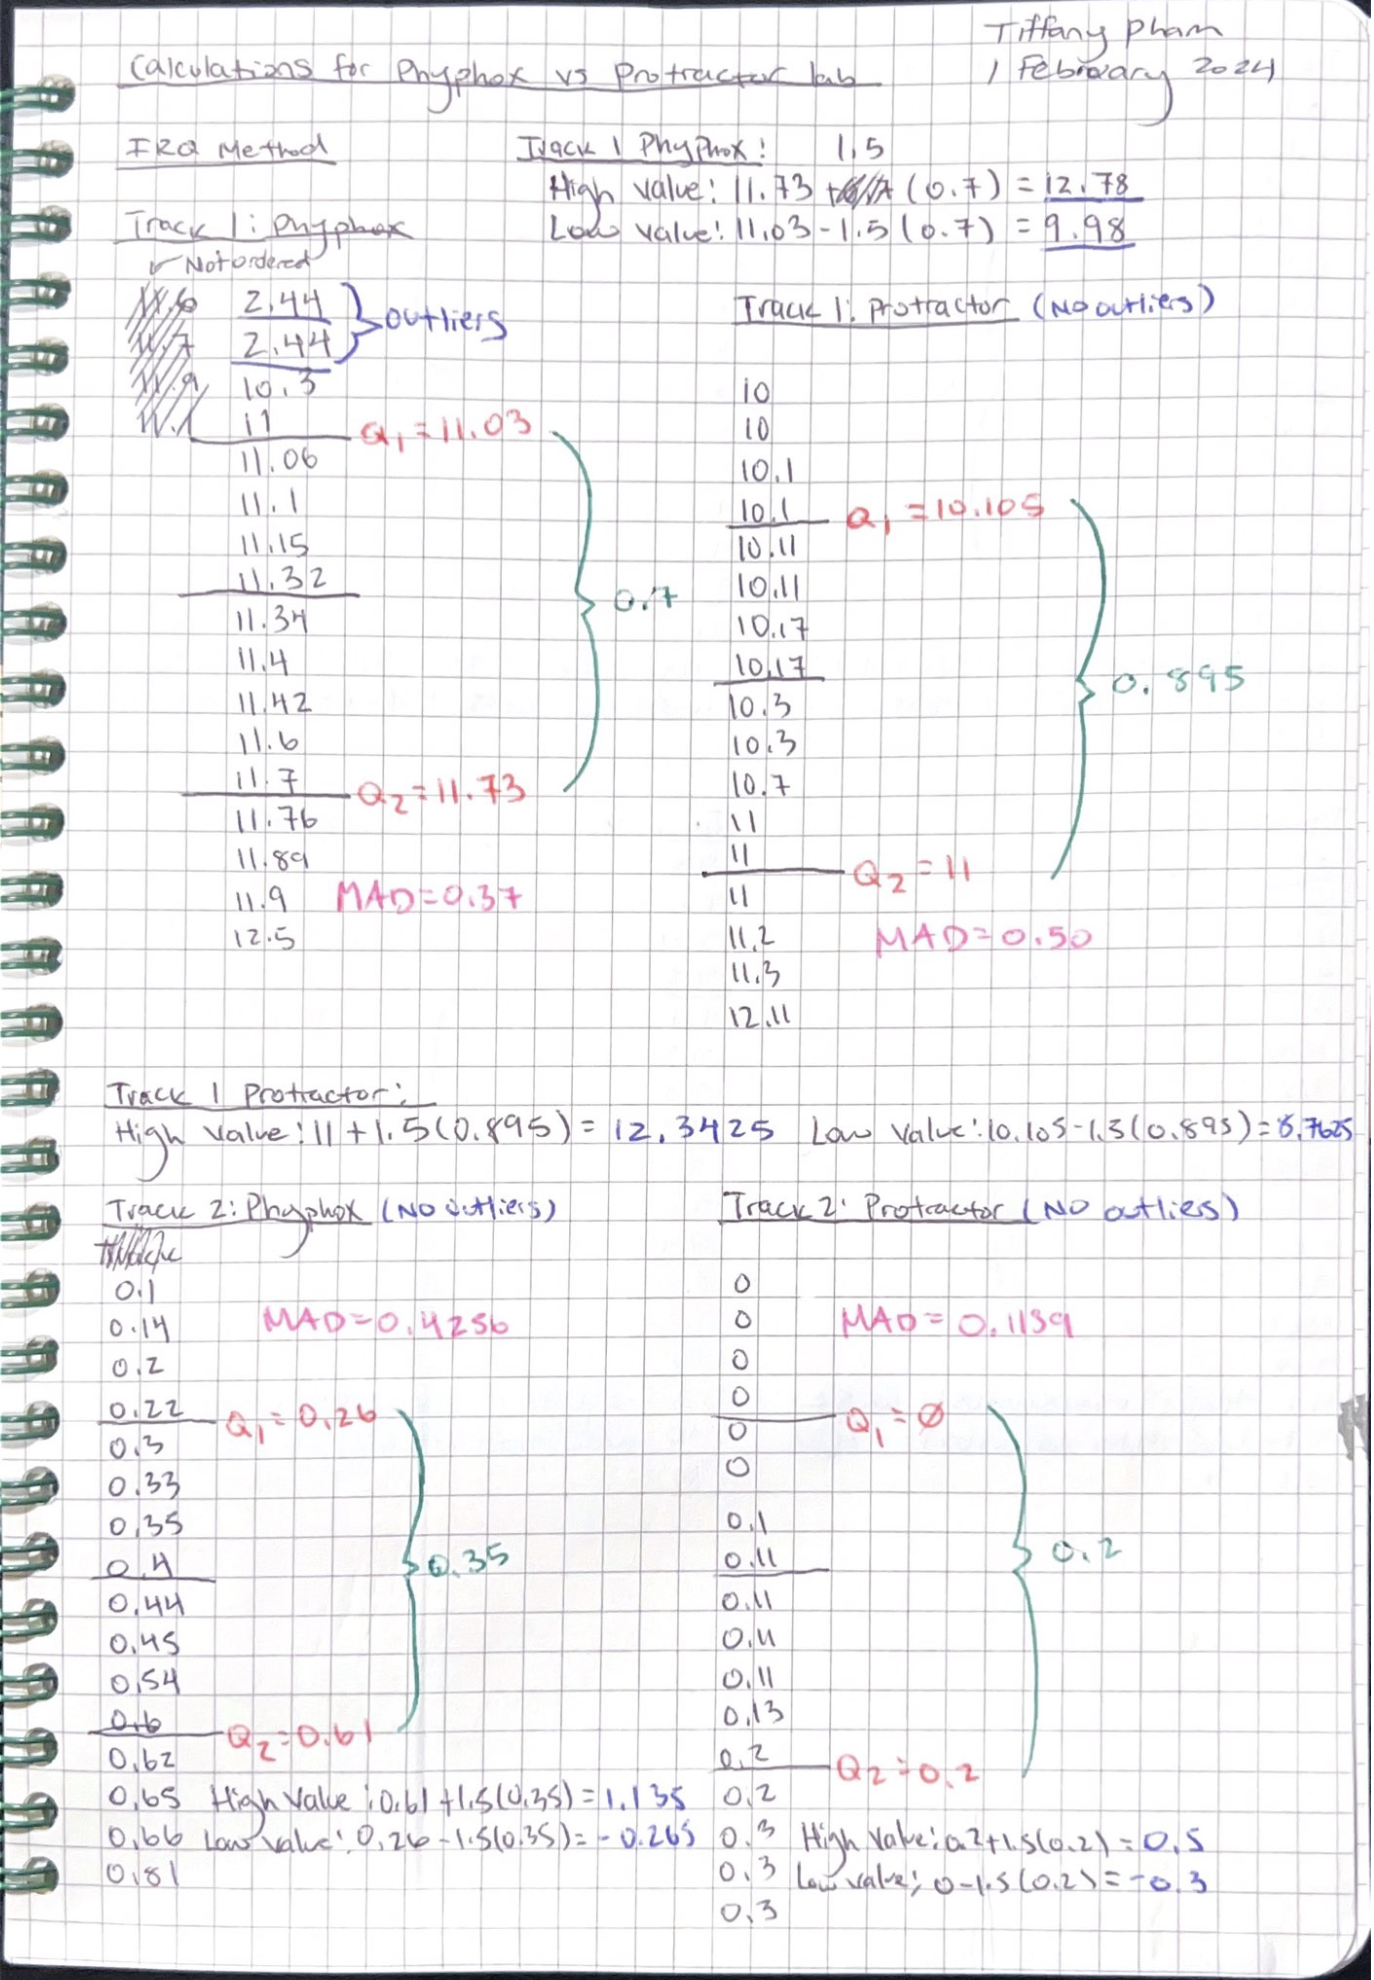
\includegraphics[width=0.8\linewidth]{images/Lab.01/PhyProTrack1-2.png}
\end{center}
\caption{Calculations of IRQ, high values, low values and MAD for tracks 1-2}
\label{fig:Track1-2PhyphoxProtractor}
\end{figure}

\begin{figure}[H] % Example of including images
\begin{center}
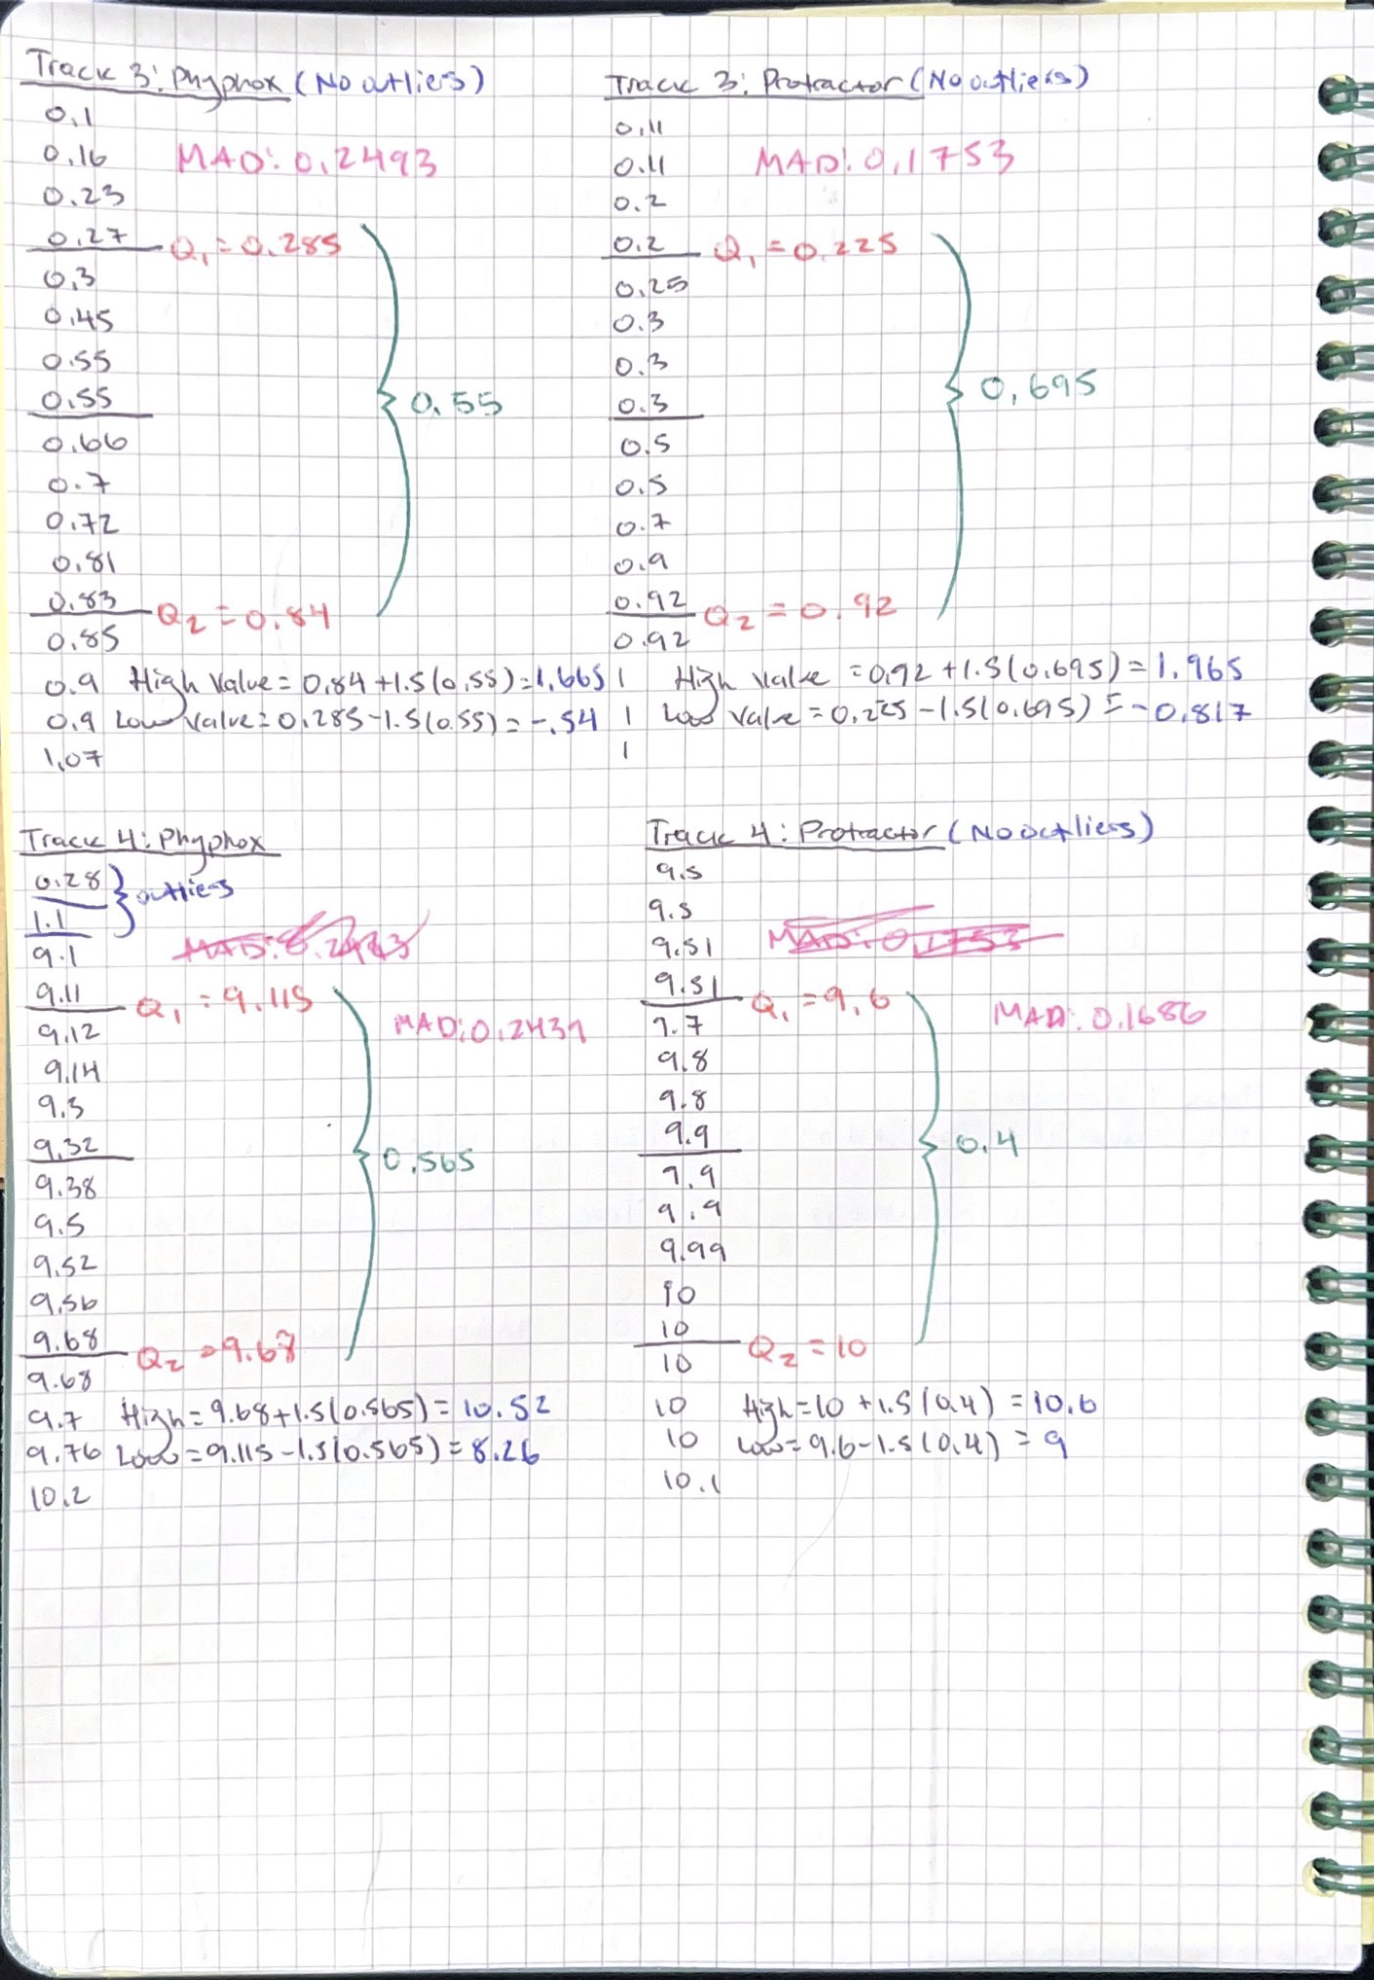
\includegraphics[width=0.9\linewidth]{images/Lab.01/PhyProTrack3-4.png}
\end{center}
\caption{Calculations of IRQ, high values, low values and MAD for tracks 3-4}
\label{fig:Track3-4PhyphoxProtractor}
\end{figure}

\begin{figure}[H] % Example of including images
\begin{center}
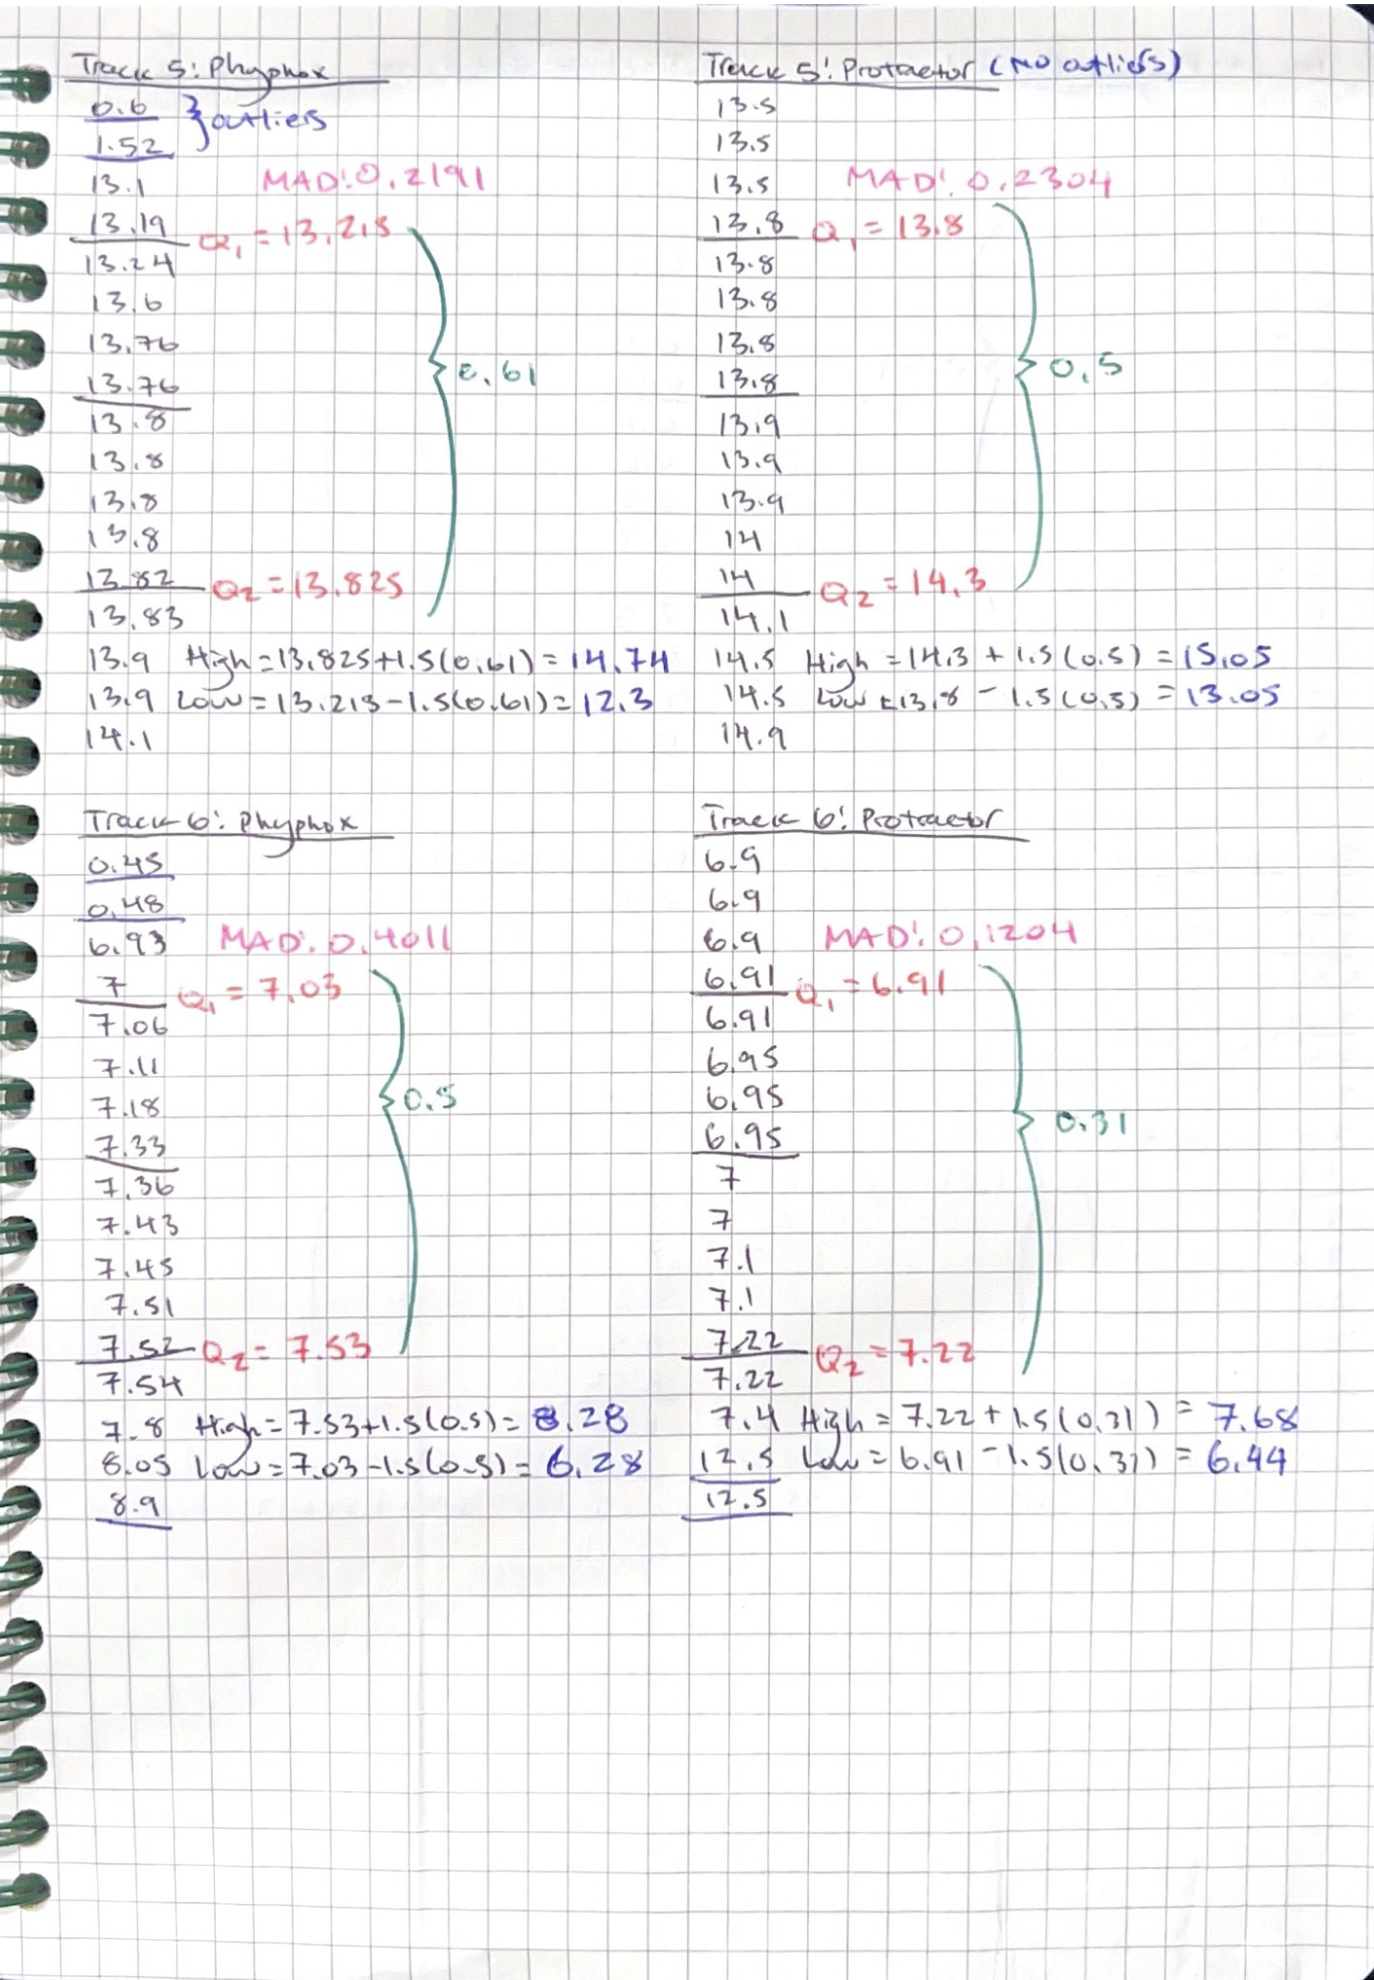
\includegraphics[width=0.9\linewidth]{images/Lab.01/PhyProTrack5-6.png}
\end{center}
\caption{Calculations of IRQ, high values, low values and MAD for tracks 5-6}
\label{fig:Track5-6PhyphoxProtractor}
\end{figure}

\begin{figure}[H] % Example of including images
\begin{center}
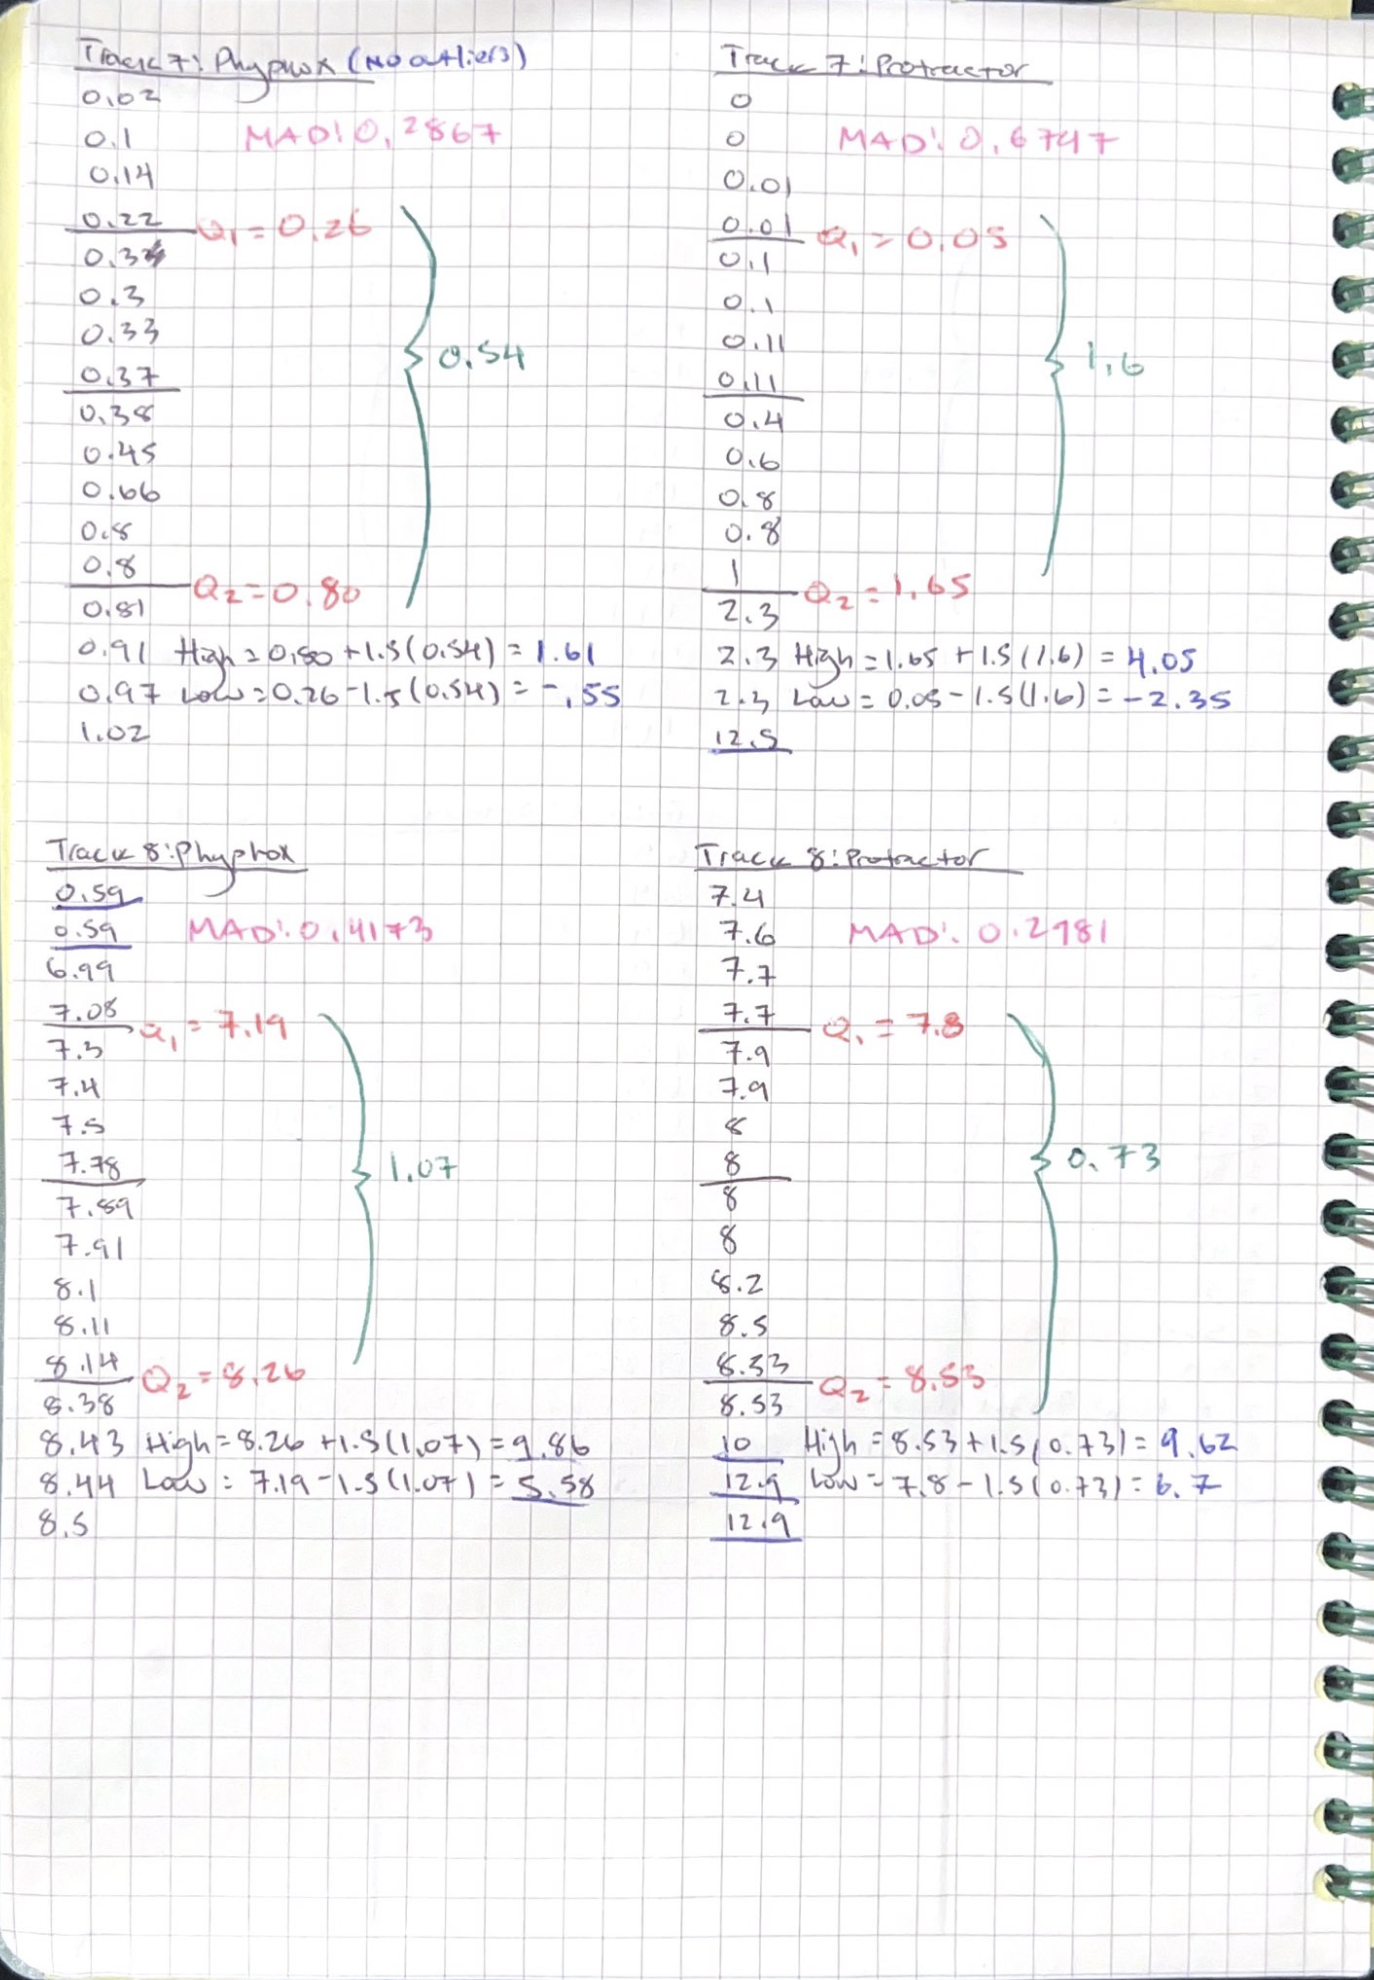
\includegraphics[width=0.9\linewidth]{images/Lab.01/PhyProTrack7-8.png}
\end{center}
\caption{Calculations of IRQ, high values, low values and MAD for tracks 7-8}
\label{fig:Track7-8PhyphoxProtractor}
\end{figure}

\begin{figure}[H] % Example of including images
\begin{center}
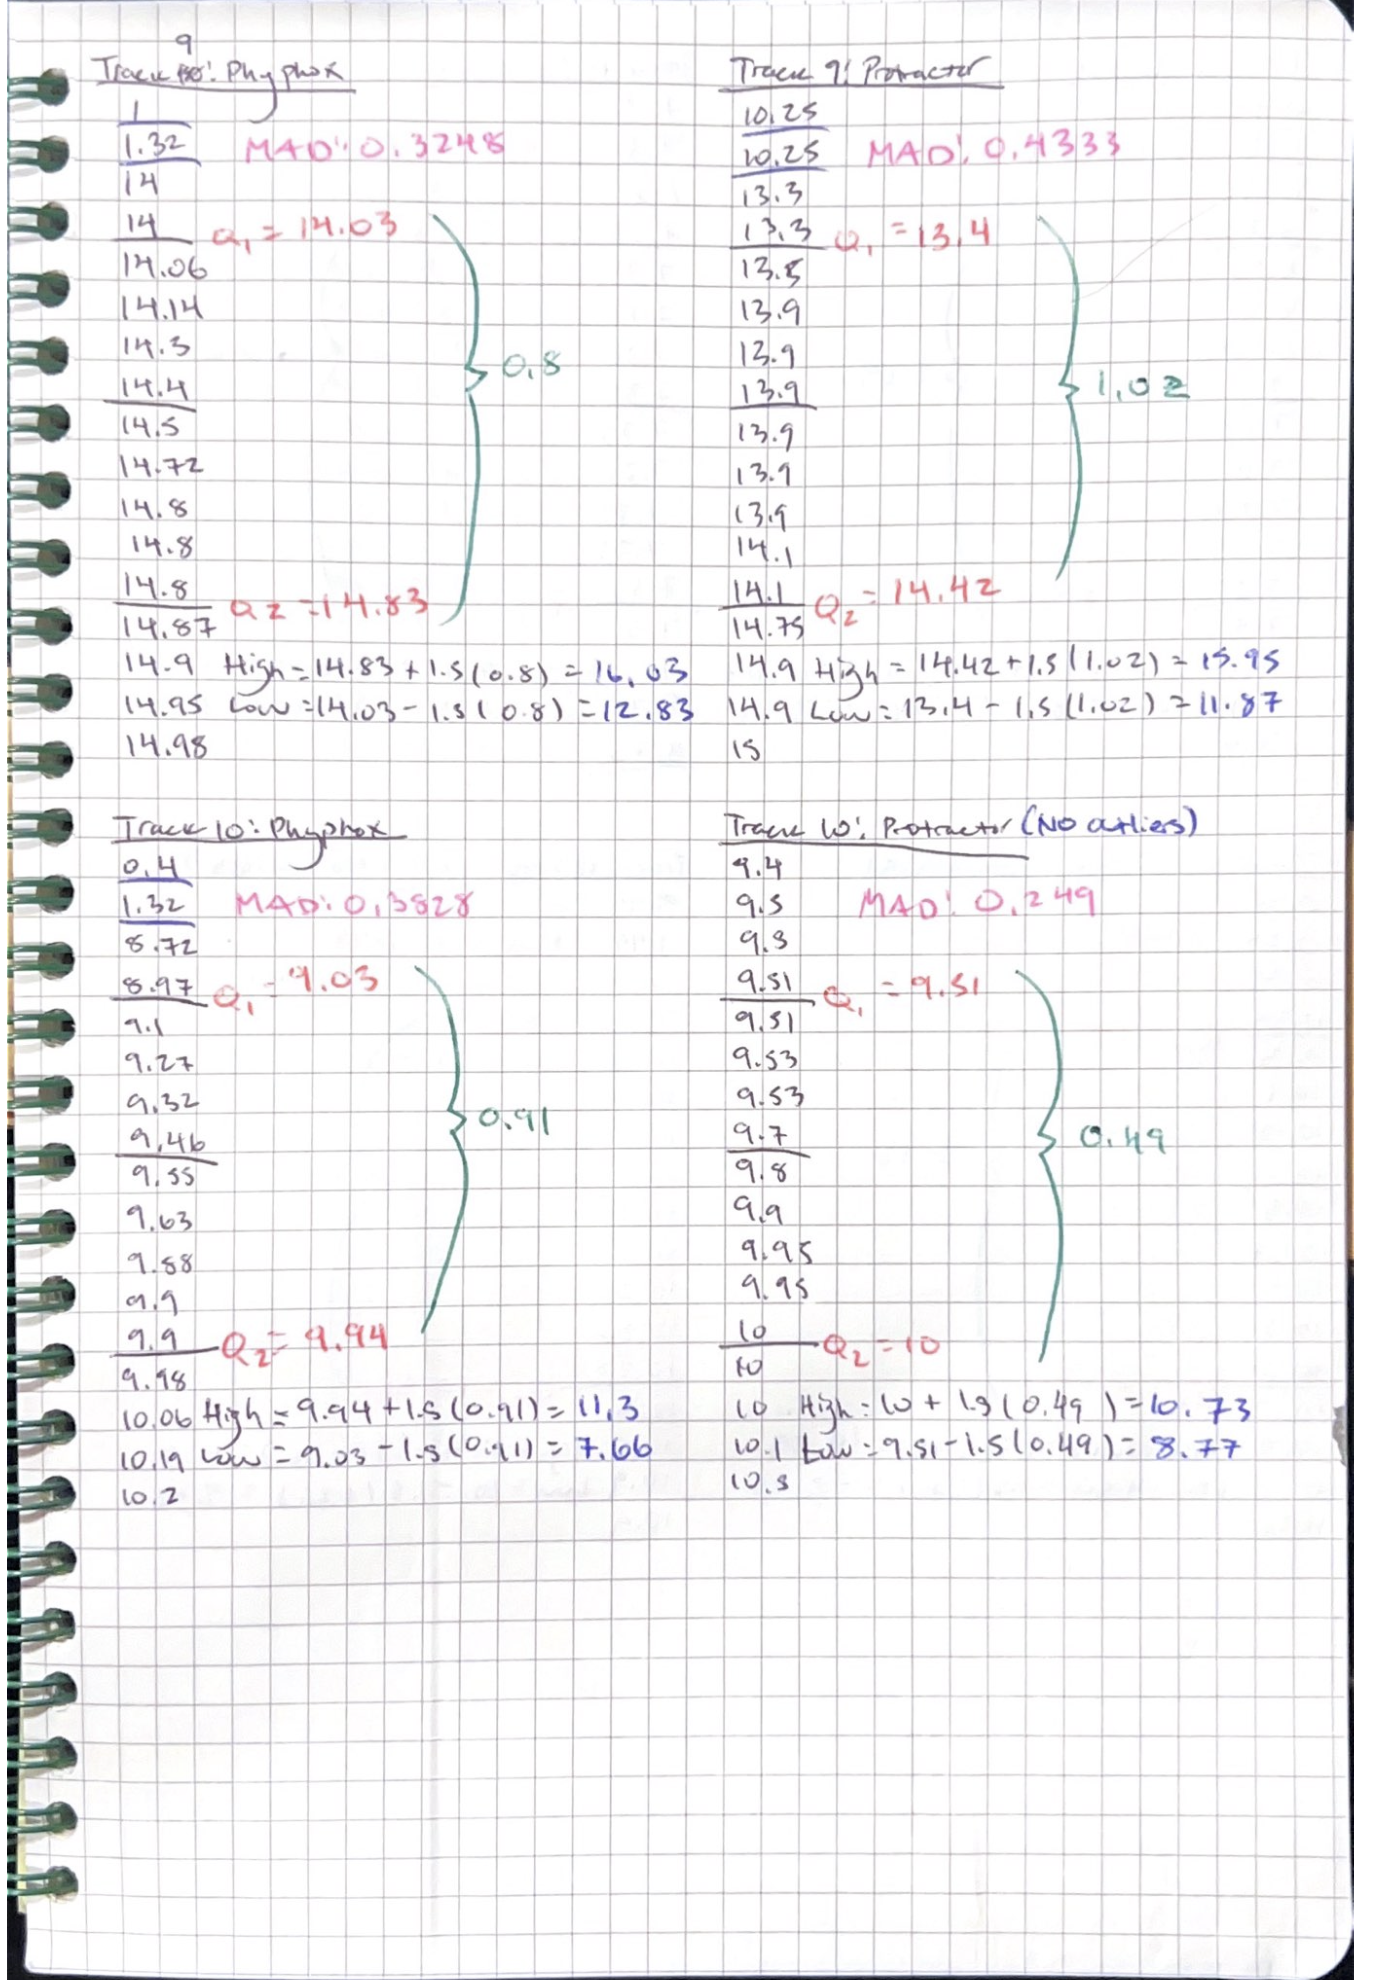
\includegraphics[width=0.9\linewidth]{images/Lab.01/PhyProTrack9-10.png}
\end{center}
\caption{Calculations of IRQ, high values, low values and MAD for tracks 9-10}
\label{fig:Track9-10PhyphoxProtractor}
\end{figure}

\begin{figure}[H] % Example of including images
\begin{center}
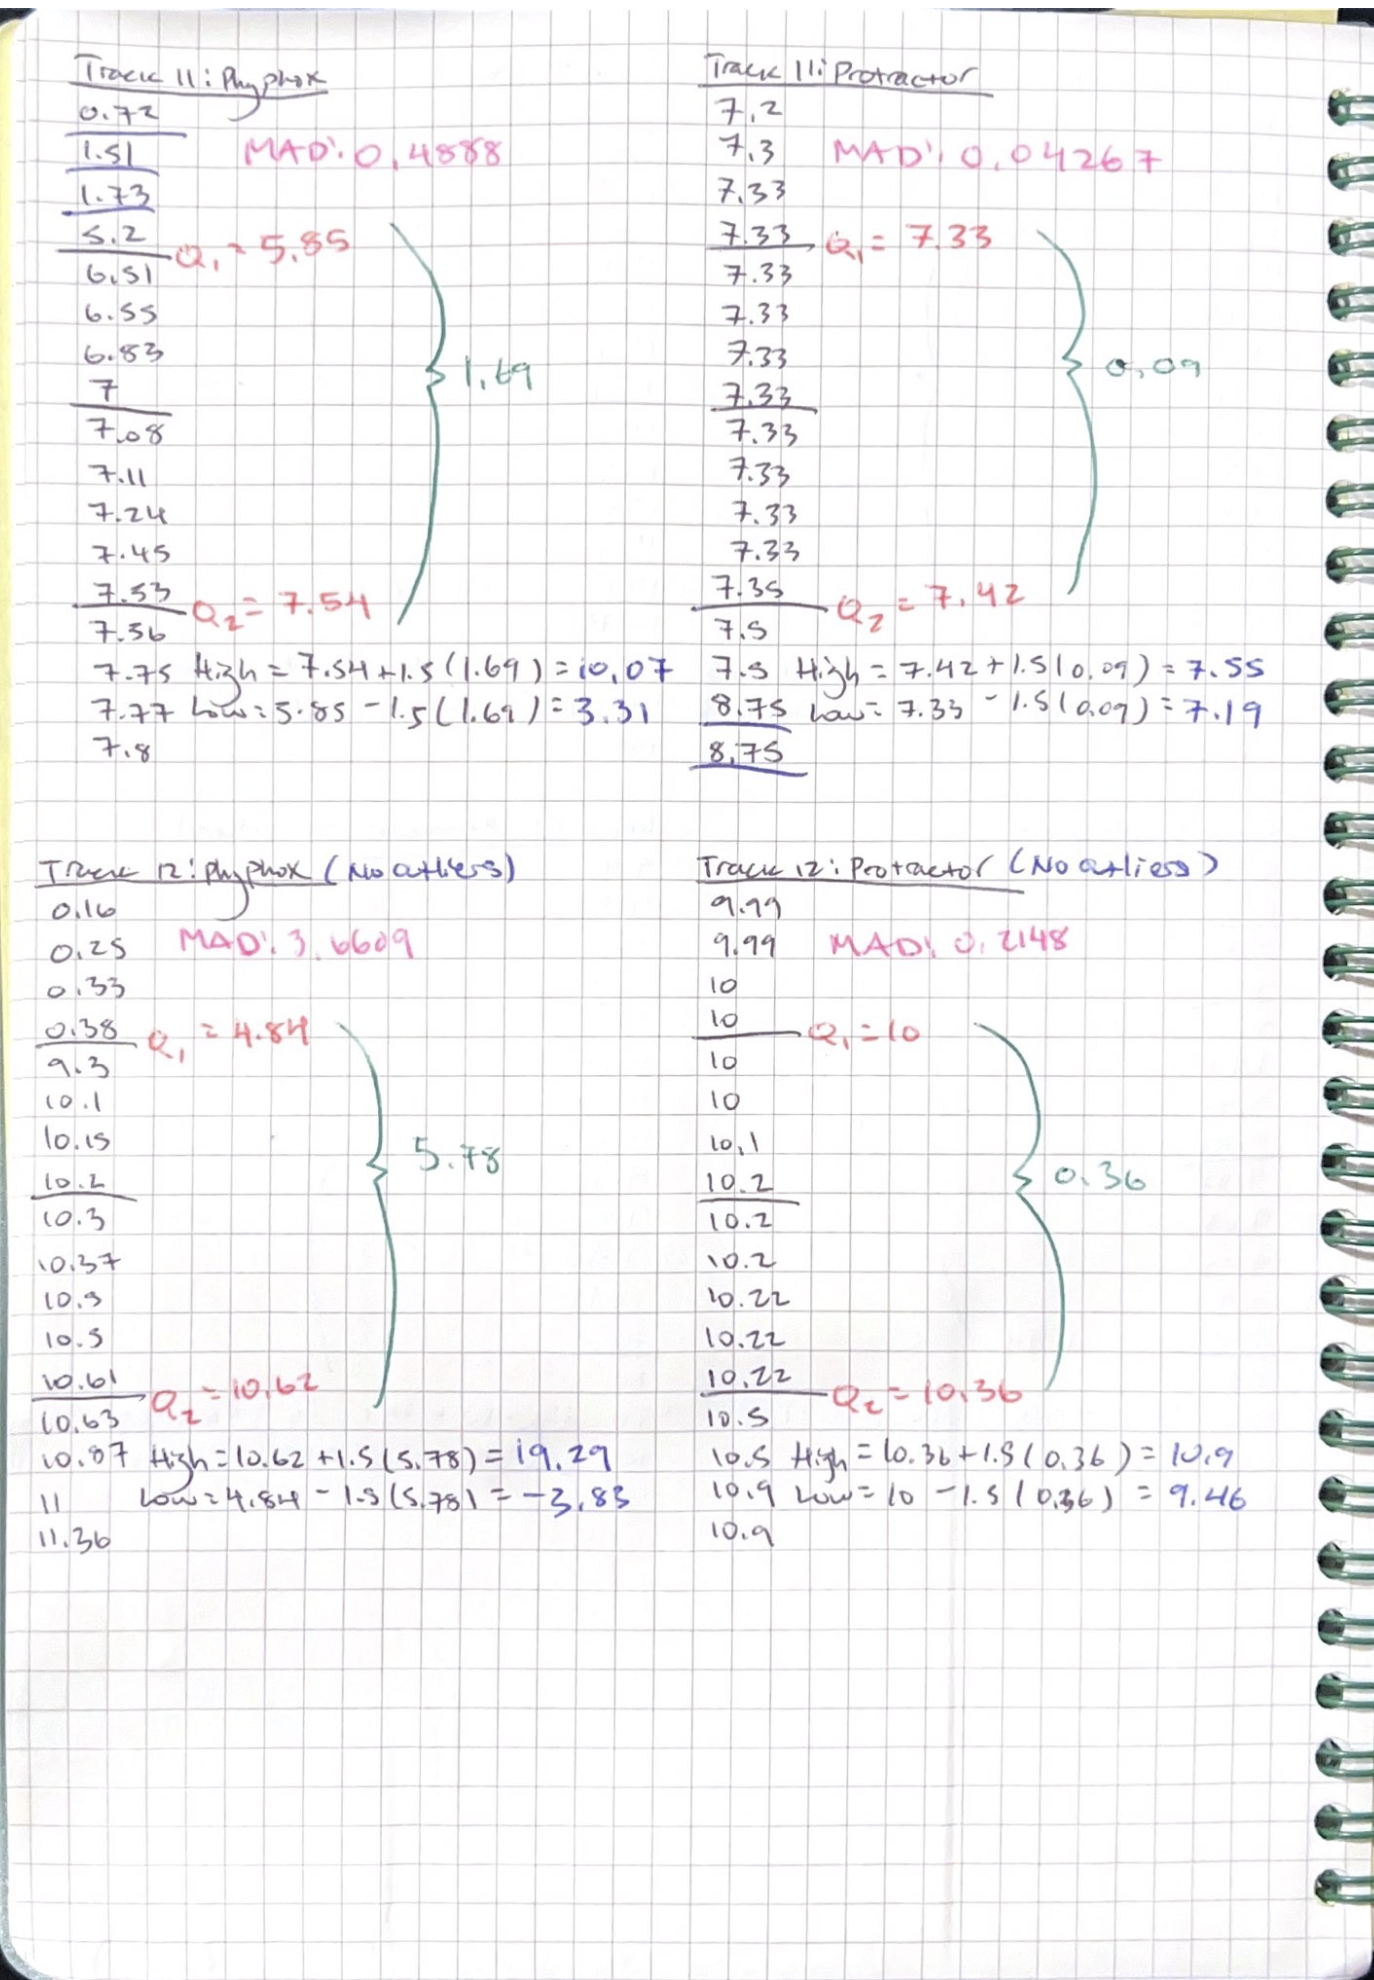
\includegraphics[width=0.9\linewidth]{images/Lab.01/PhyProTrack11-12.png}
\end{center}
\caption{Calculations of IRQ, high values, low values and MAD for tracks 11-12}
\label{fig:Track11-12PhyphoxProtractor}
\end{figure}

\begin{figure}[H] % Example of including images
\begin{center}
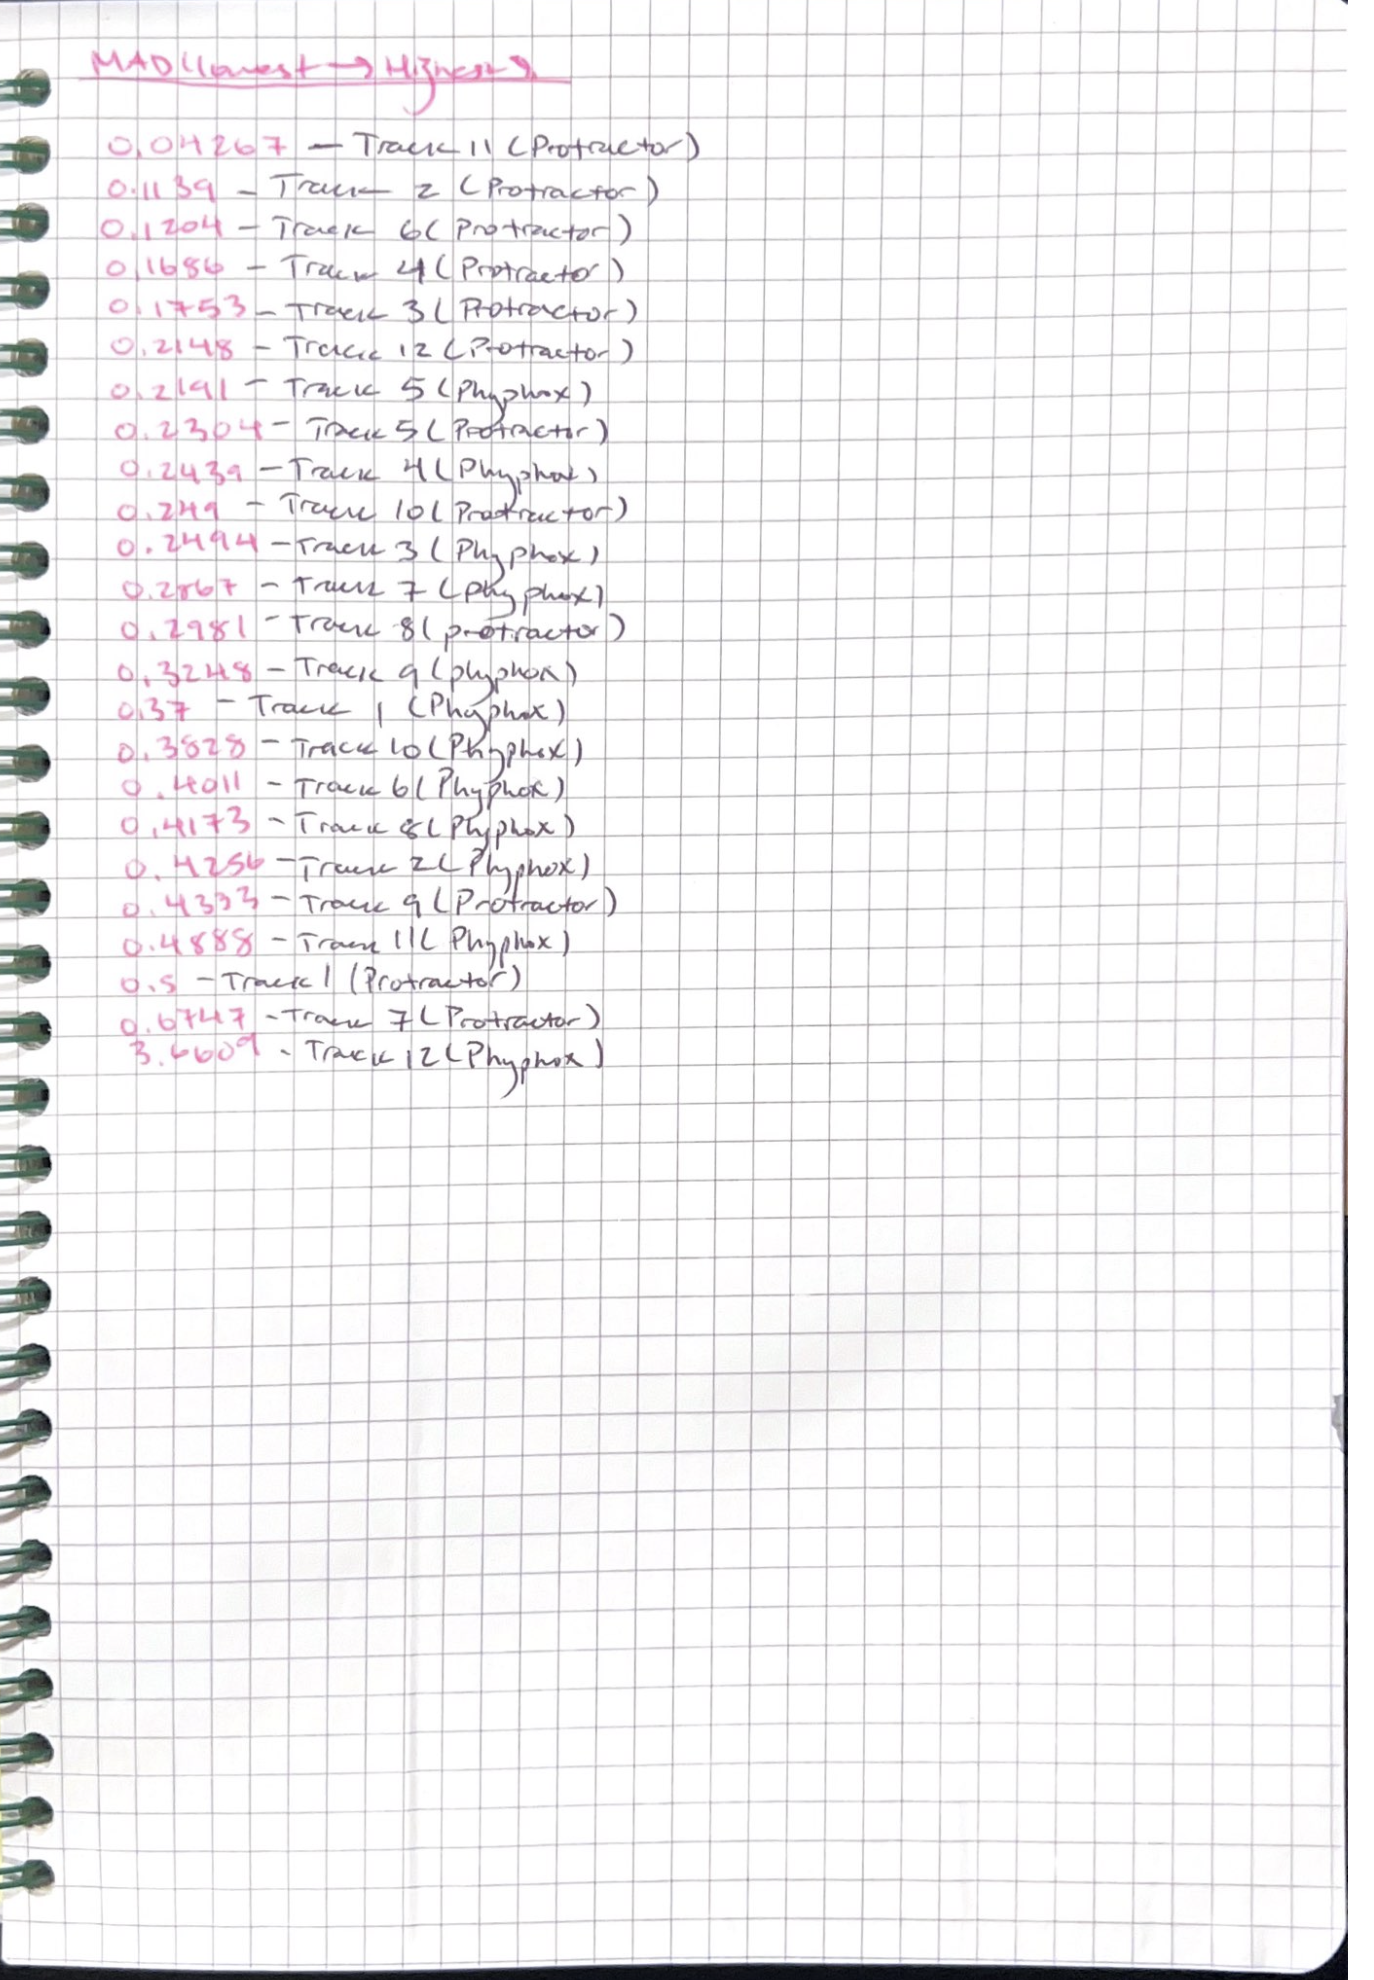
\includegraphics[width=0.9\linewidth]{images/Lab.01/PhyProMADLH.png}
\end{center}
\caption{MAD data for all tracks from lowest to highest}
\label{fig:MADLHPhyphoxProtractor}
\end{figure}

%----------------------------------------------------------------------------------------

\experiment{Lab Notebook Prompts}
\begin{enumerate}
    \item You’ll use inclined tracks in future experiments and will need measure the angle. You’re doing this experiment to decide what will be the most appropriate way(s) to do so.
    \begin{enumerate}[(a)]
        \item Based on the mean absolute deviation, what angles are most precise? Least precise? Is there a trend? \textit{This can inform if there are different conditions for track angles and phyphox vs. protractor measurements.}
        \item How do \underline{your} measurements compare to the mean and MAD? \textit{For example, do your phyphox inclination measures tend to be larger or smaller than the mean? Do your protractor readings tend to be larger or smaller? These could also inform how you choose to measure angles in the lab.}
        \item Compare the protractor and phyphox values for each angle. Considering the mean absolute deviation, do the answers agree? Are there trends in agreement or disagreement based on angle?
        \item List the pros/cons of the phyphox app and proctractor.
        \item Feel free to ask yourself additional questions or observations about the data and results.
        \item Based on the data and the data and \underline{your} measurements, under what conditions, if any, would you use the
        \begin{enumerate}[i]
            \item phyphox app?
            \item protractor?
        \end{enumerate}
    \end{enumerate}
\end{enumerate}

%----------------------------------------------------------------------------------------

\experiment{Lab Notebook Answers}
\begin{enumerate}
    \item Notebook Answers:
    \begin{enumerate}[(a)]
        \item Based on the Mean Absolute Deviation (MAD), I would conclude that \textbf{Track 11} and \textbf{Track 2} would be most precise and \textbf{Track 7} and \textbf{Track 12} would be the least precise. There doesn't seem to be a trend, but if you do count the individual tracks separately for Phyphox and Protractor, then it seems that the Protractor runs are the most precise compared to the Phyphox runs.
        \item There were some readings that were way out of range compared to the mean, some of them tended to be larger than the mean.
        \item After comparing the Phyphox and Protractor values, I found that the MAD was always bigger then the protractor values in general. There seems to be a trend on the angles as when the Phyphox app says the angle is smaller, so does the Protractor, when the Phyphox app says the angle is bigger, so does the Protractor, and vice versa.
        \item The pro of the protractor is that you will know that the readings you get will be accurate or within the range of $\pm2$. But because the protractor isn't digital compared to the Phyphox, you will have to guess what value the leg is on as it will be difficult to determine precisely what value the leg is on. Unlike the protractor the pro of the Phyphox app is that the readings are digital; it will tell the exact value and you won't have to guess what value it will be on as it is show on the screen. So it is easy to read the data. But a con is that the values will most likely have a high MAD and that the readings would vary a lot.
        \item N/A
        \item Phyphox App vs Protractor:
        \begin{enumerate}[i]
            \item I would use the Phyphox App if I just needed a quick measurement of any angle.
            \item I would use the protractor if I enough time to get a more accurate reading.
        \end{enumerate}
    \end{enumerate}
\end{enumerate}

%----------------------------------------------------------------------------------------

\labday{Wednesday, 07 February 2024}
\vspace{-5mm}
Tiffany Pham

\experiment{Lab 03 (Lab) - Logger Pro}
\textbf{Purpose}
\begin{enumerate}
    \item Become familiar with lab equipment (Logger Pro, Track, Vernier).
    \item Gain experience collecting and analyzing real data and making reasoned, supported conclusions on what that data means.
    \item Practice recording what you’re doing and why in your lab notebook.
\end{enumerate}

\hfill \break
\textbf{Objective}

Interpret the LoggerPro data, relating it to the cart's motion.

\hfill \break
\textbf{Predictions}

I predict that the motion detector will be able to interpret the data accurately and show when the track is moving away from the sensor and when it is getting closer to it.

\hfill \break
\textbf{Procedure}
\begin{enumerate}
    \item Turn on the computer or laptop and go to the Logger Pro application.
    \item Set up the track, cart, and motion detector if it isn't set up already. Make sure the magnets (grey end) face away from the motion detector, and do not let the cart crash into the motion detector.
    \item When increasing the angle of the track, make sure the legs at the bottom end are supporting it (rather than the metal tab that holds the bumper).
    \item If you let the cart bounce off the bumper at the far end of the track (away from the motion detector), make sure the cart stays in the track grooves. Have someone at the bumper end of the track to catch the cart, just in case.
    \item Start the multiple runs to measure the data. From top to bottom - hold the cart at the top and let it go down. From bottom to top - push the cart with just the right amount of force so that it can go to the motion detector but not enough force to hit it.
\end{enumerate}

\hfill \break
What could go wrong:
\begin{itemize}
    \item Cart hitting the motion detector
    \item Cart falling off the track
    \item Not pushing it with enough force
    \item Motion detector not being angled correctly
\end{itemize}

\hfill \break
\textbf{Equipment needed}
\begin{itemize}
    \item Computer/ Laptop
    \item Logger Pro
    \item Vernier
    \item Motion Detector
    \item Track
    \item Cart
\end{itemize}

%----------------------------------------------------------------------------------------

\newpage
\hfill \break
\experiment{Cart Data}
\begin{figure}[H] % Example of including images
\begin{center}
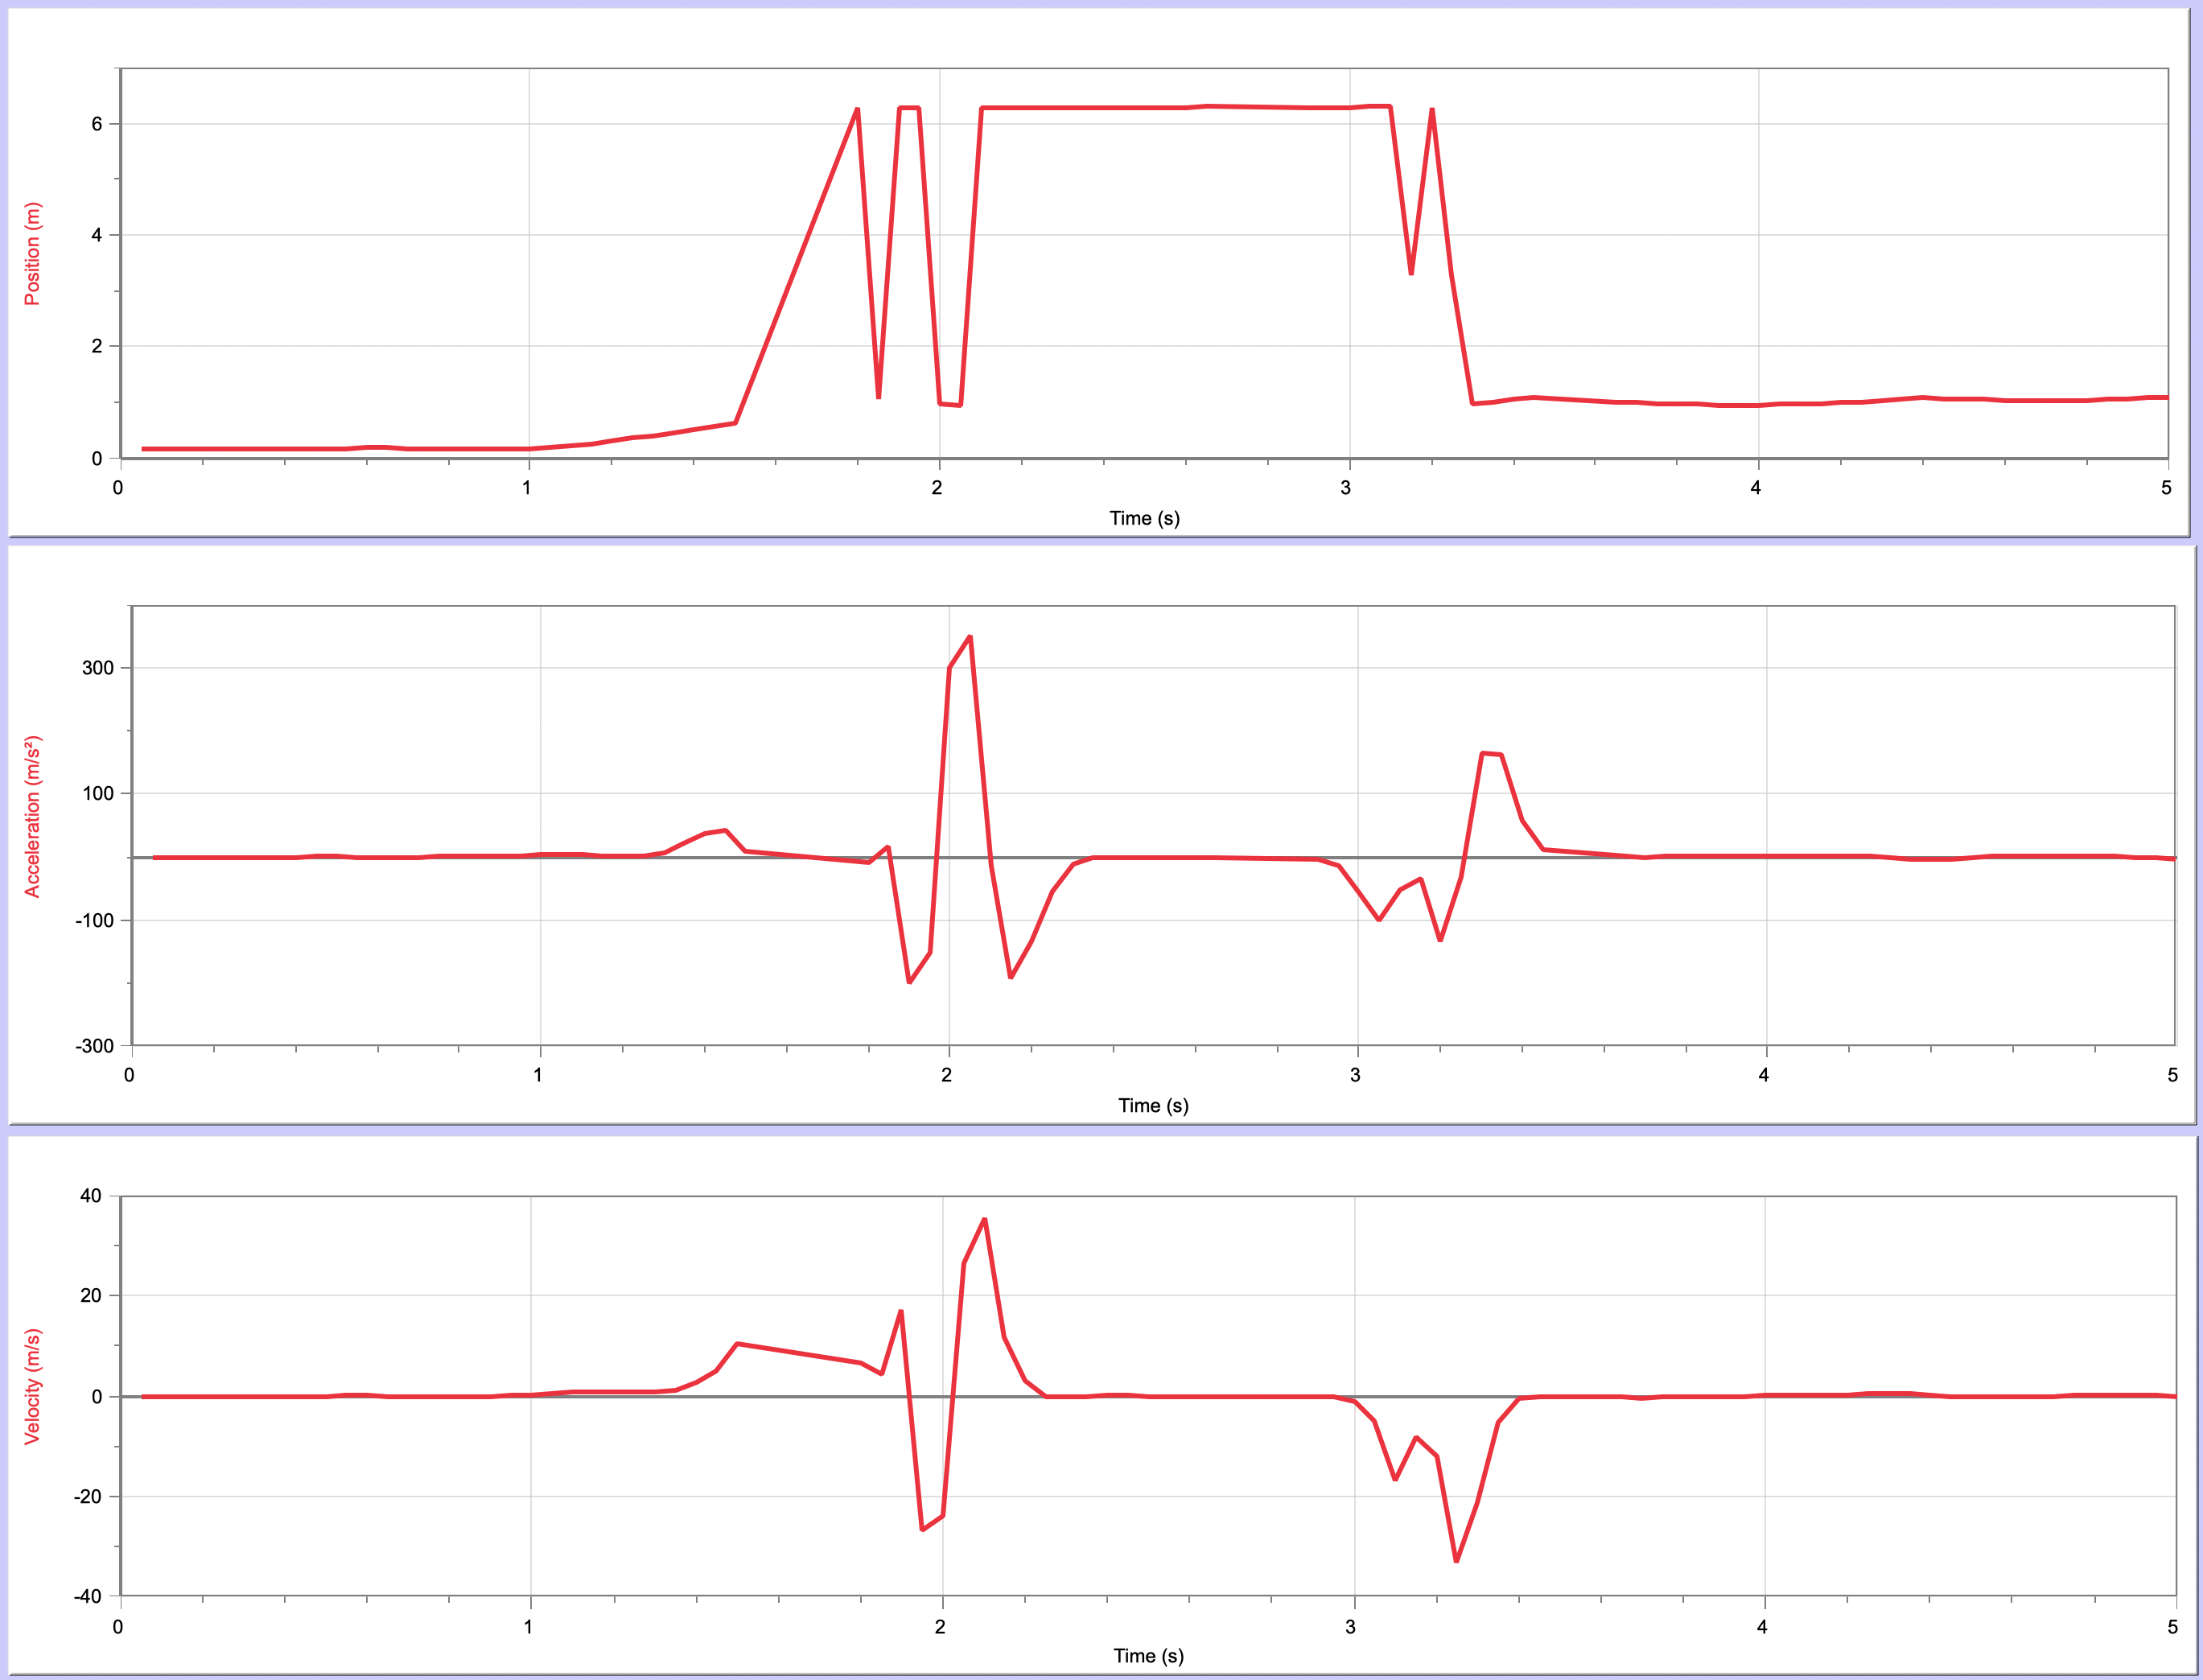
\includegraphics[width=1\linewidth]{images/Lab.02/GoDown1.png}
\end{center}
\caption{Run 1 of 3 from cart going from top of track to bottom of track}
\label{fig:Data of Cart GoDown1}
\end{figure}

\begin{figure}[H] % Example of including images
\begin{center}
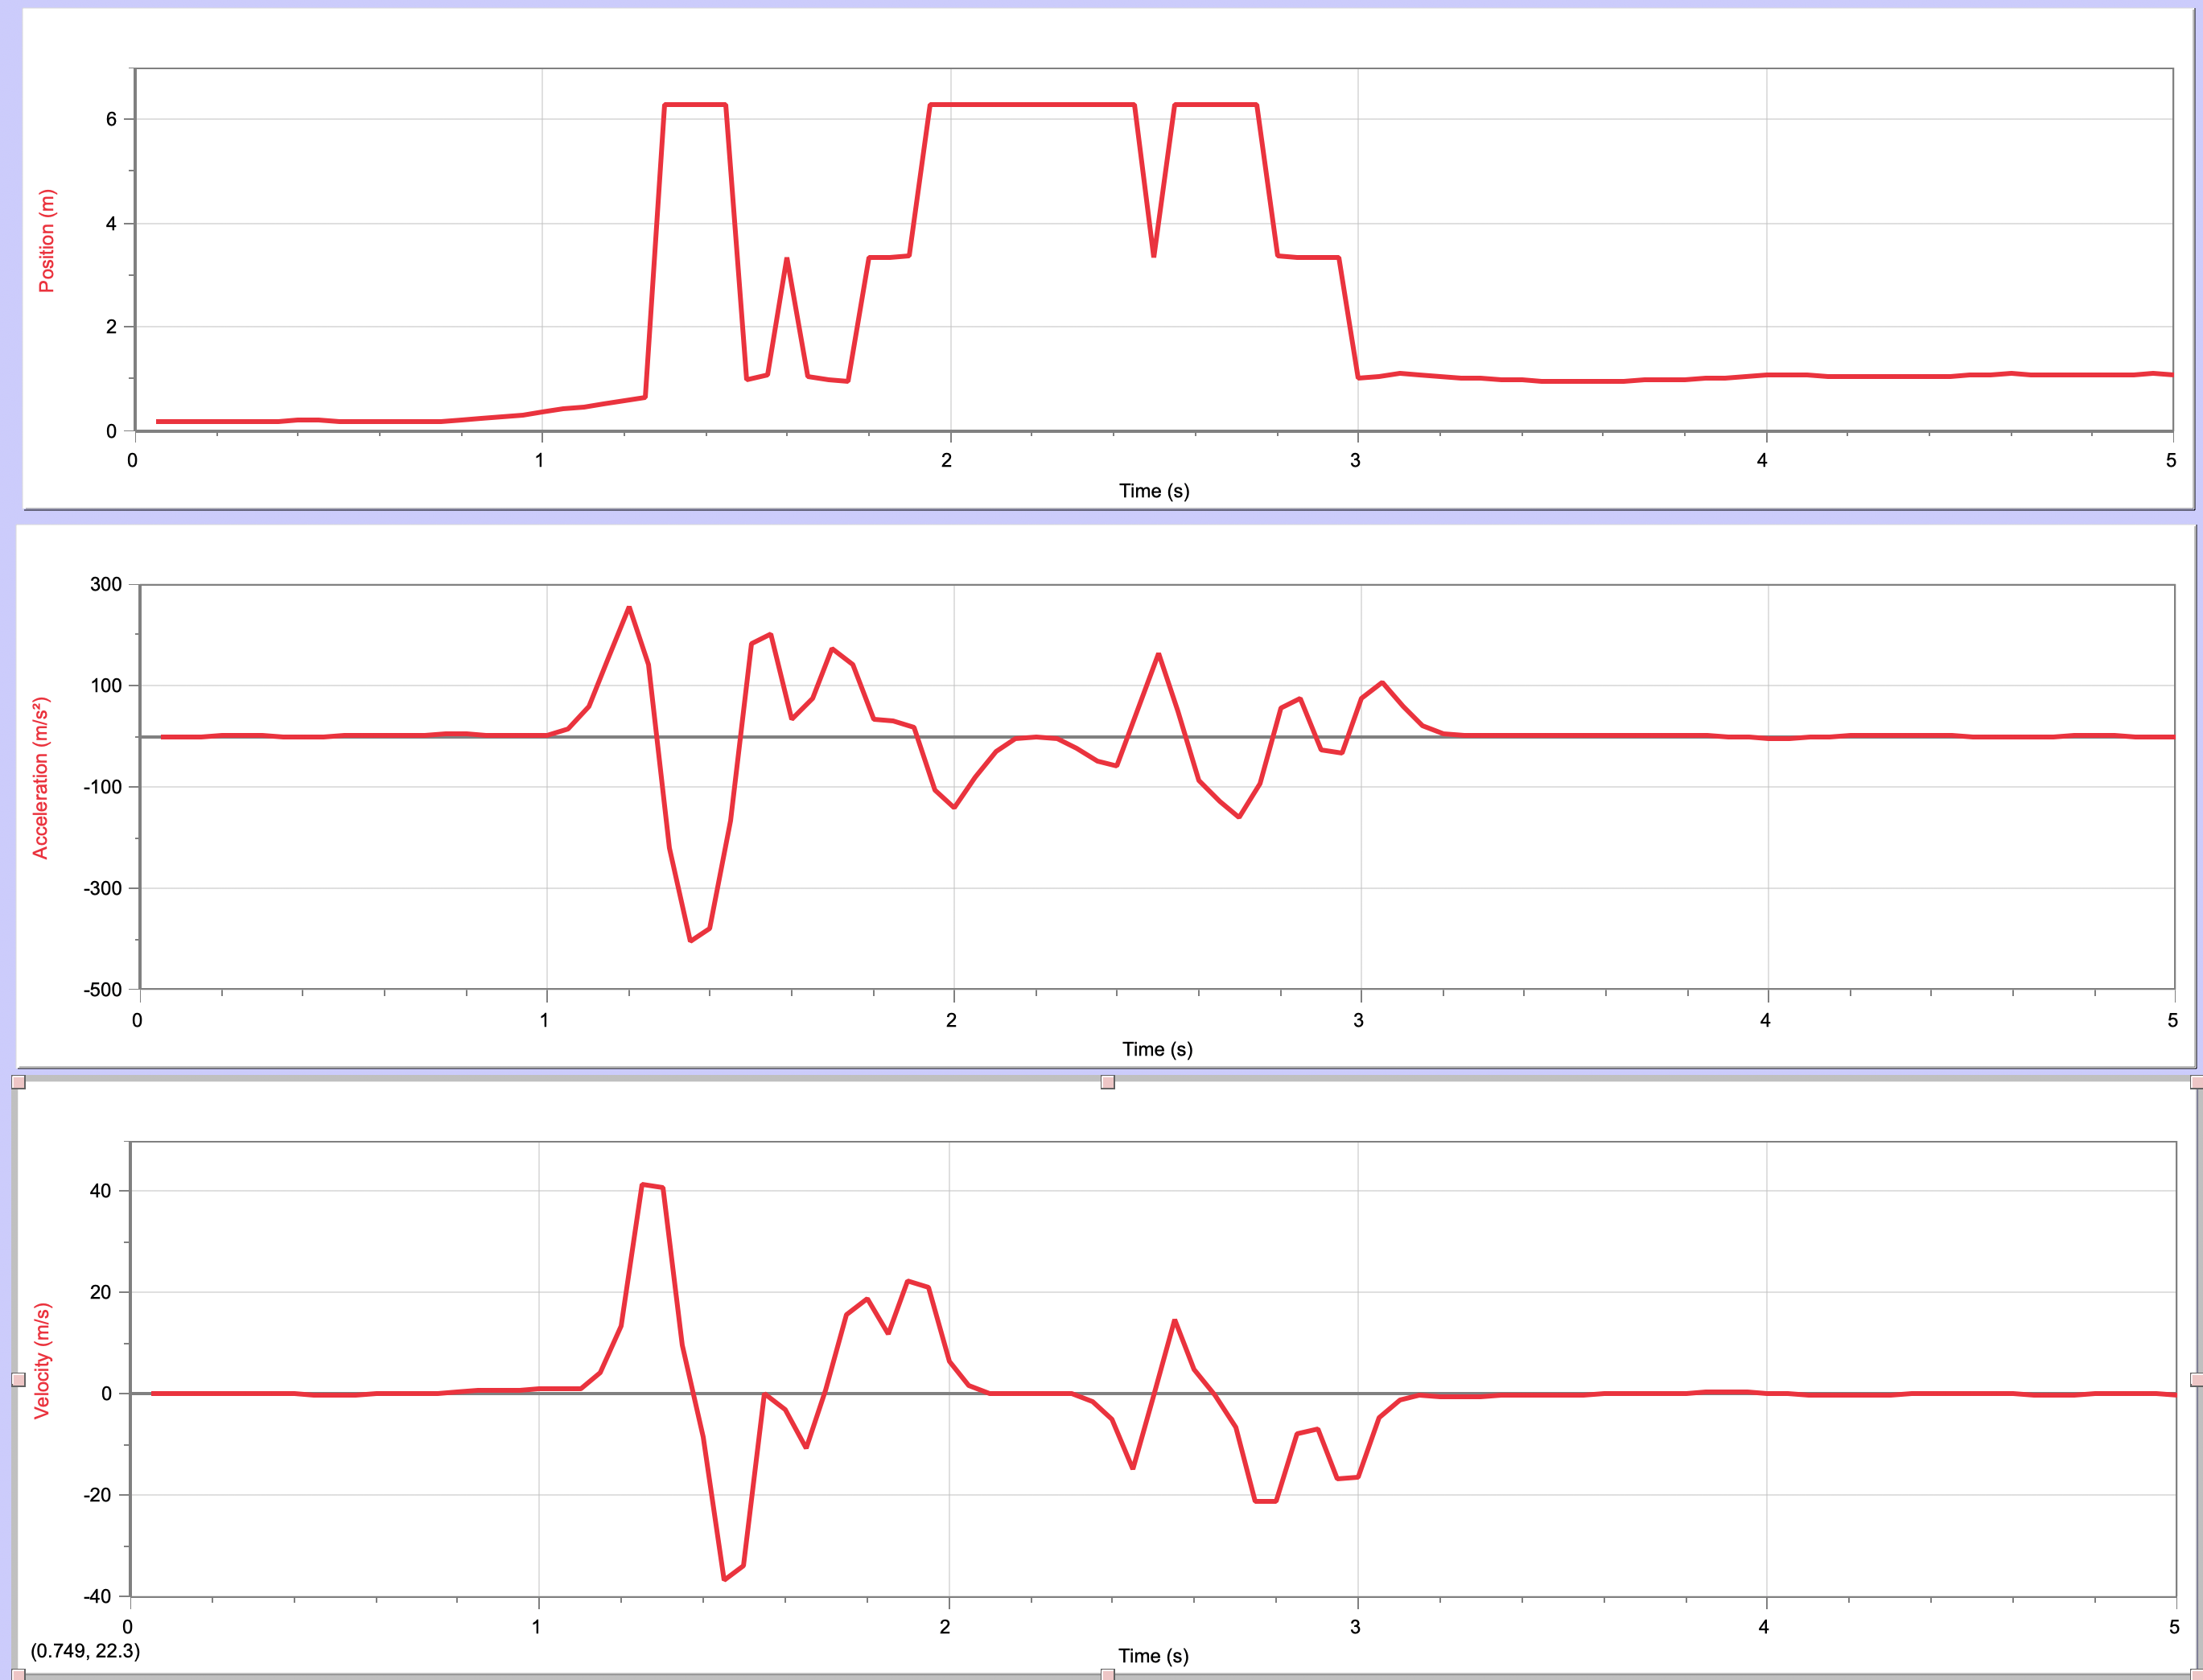
\includegraphics[width=1\linewidth]{images/Lab.02/GoDown2.png}
\end{center}
\caption{Run 2 of 3 from cart going from top of track to bottom of track}
\label{fig:Data of Cart GoDown2}
\end{figure}

\begin{figure}[H] % Example of including images
\begin{center}
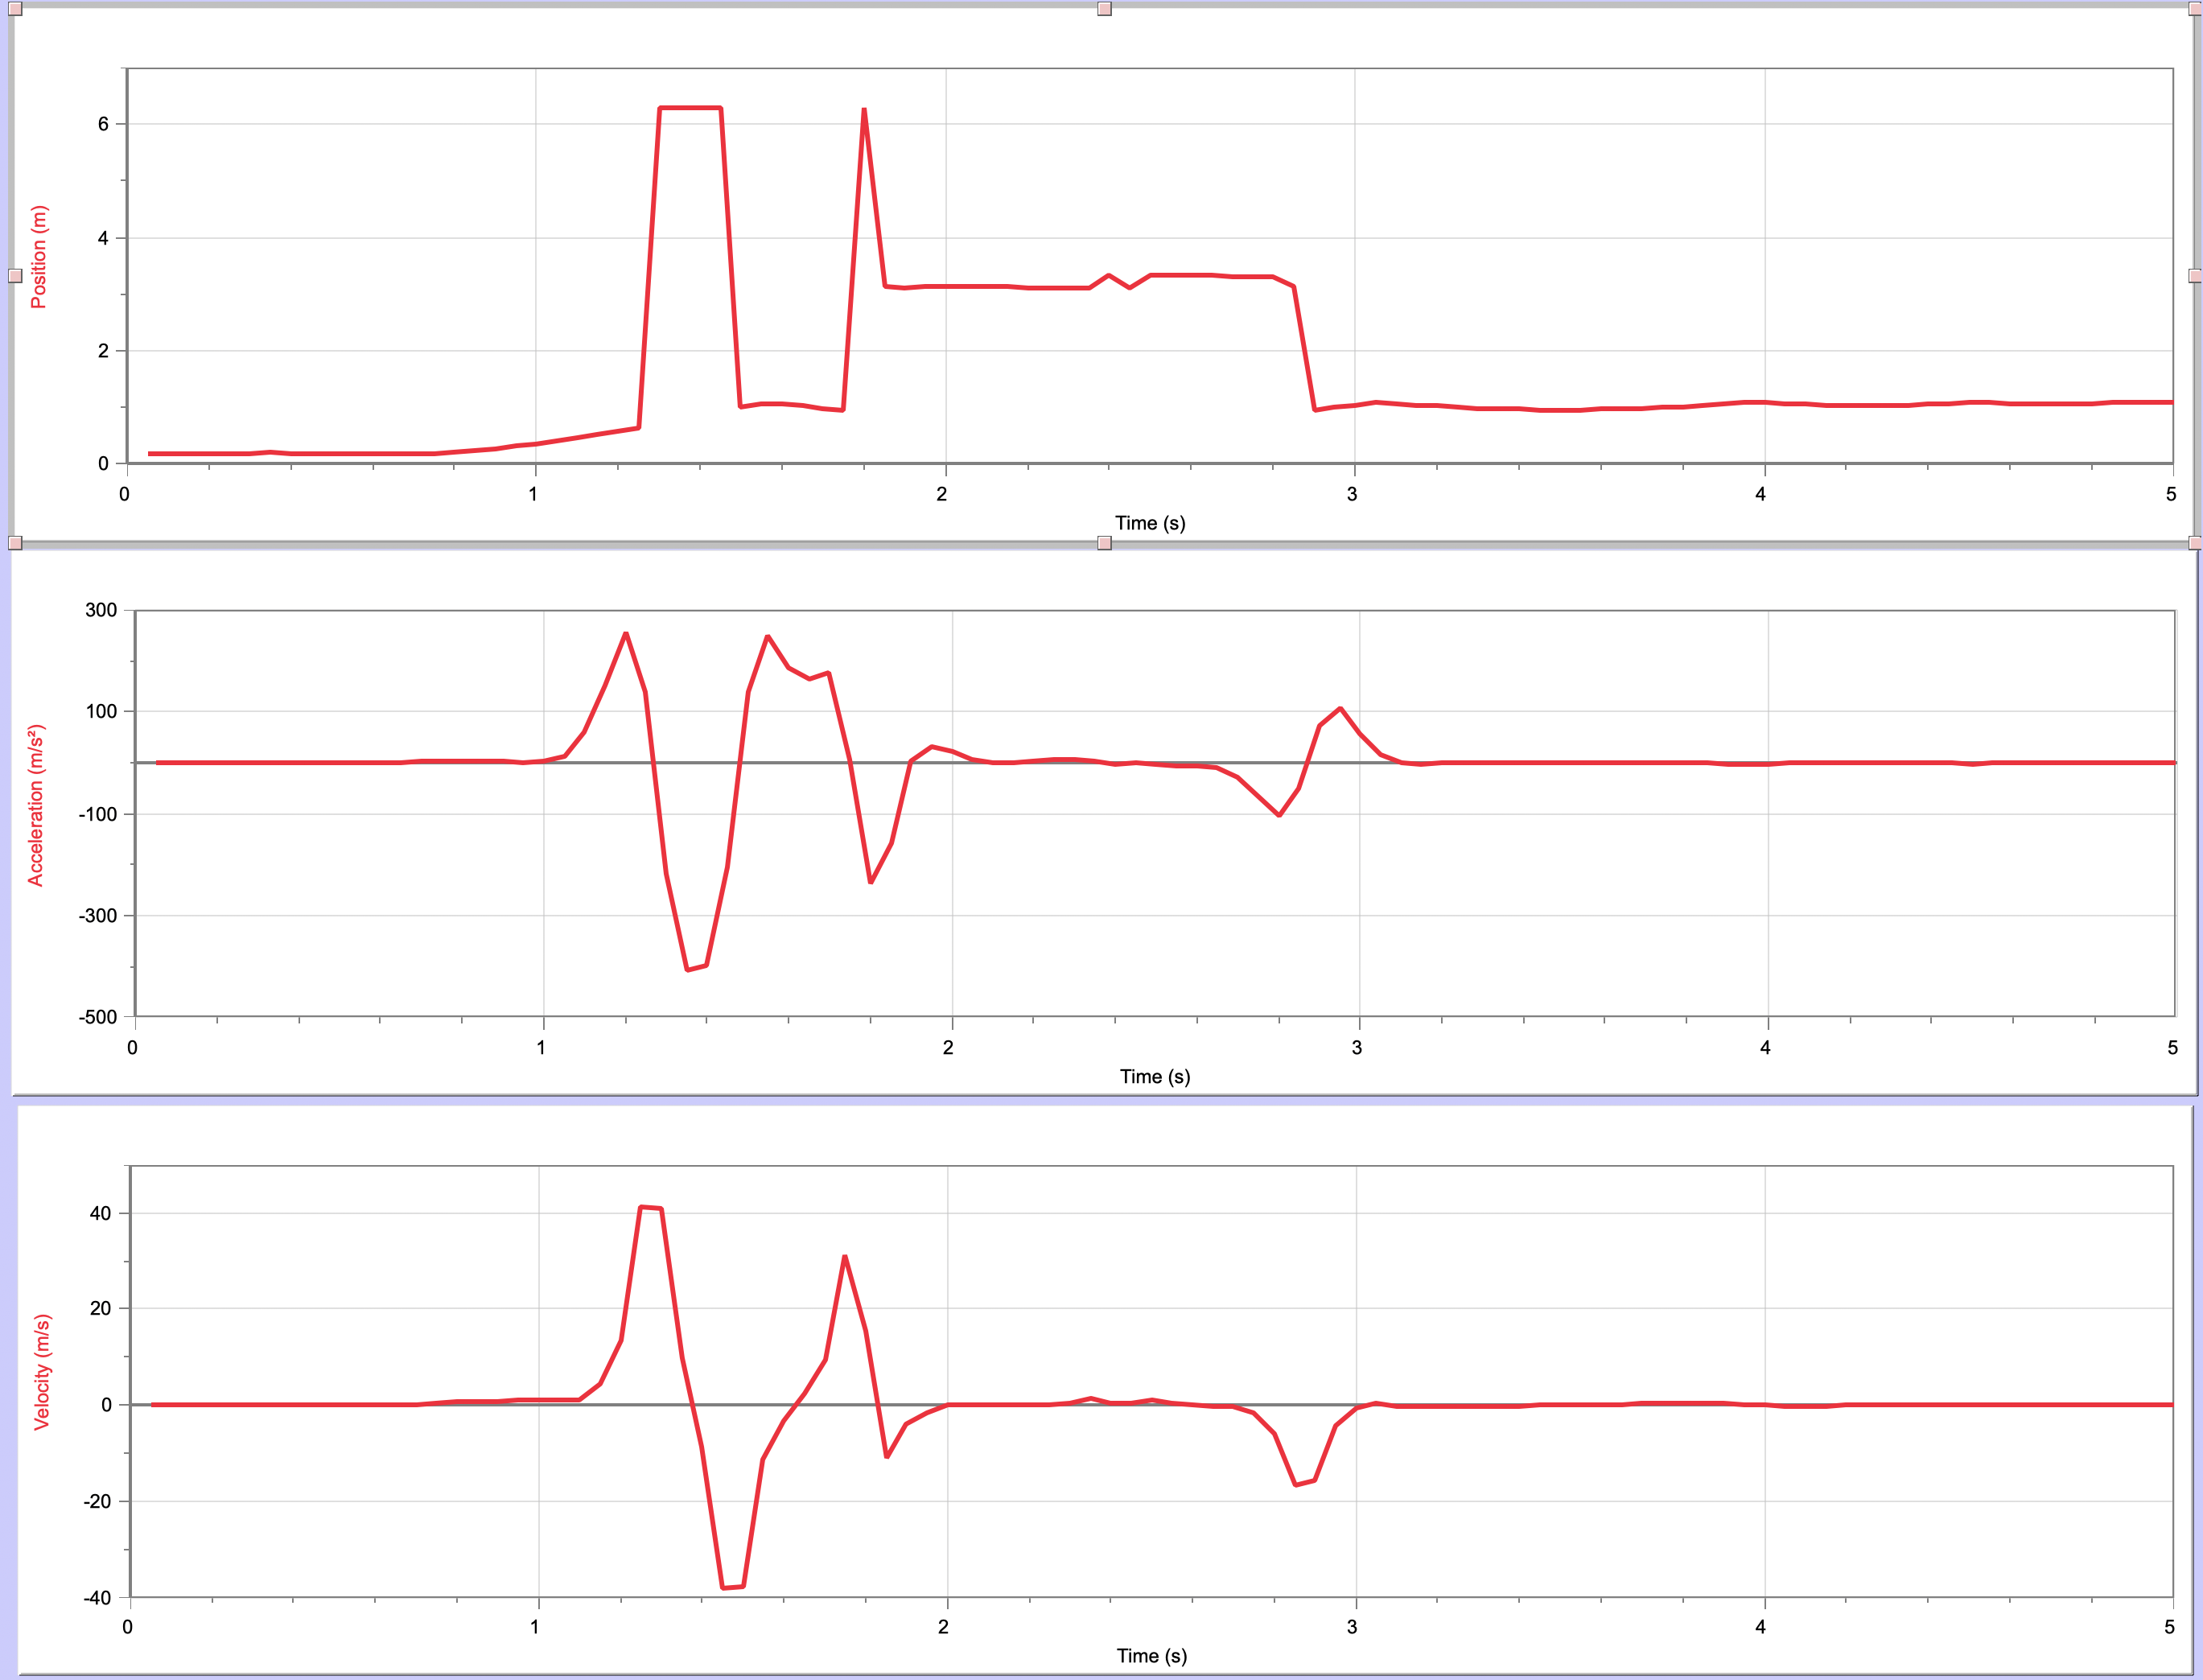
\includegraphics[width=1\linewidth]{images/Lab.02/GoDown3.png}
\end{center}
\caption{Run 3 of 3 from cart going from top of track to bottom of track}
\label{fig:Data of Cart GoDown3}
\end{figure}

\begin{figure}[H] % Example of including images
\begin{center}
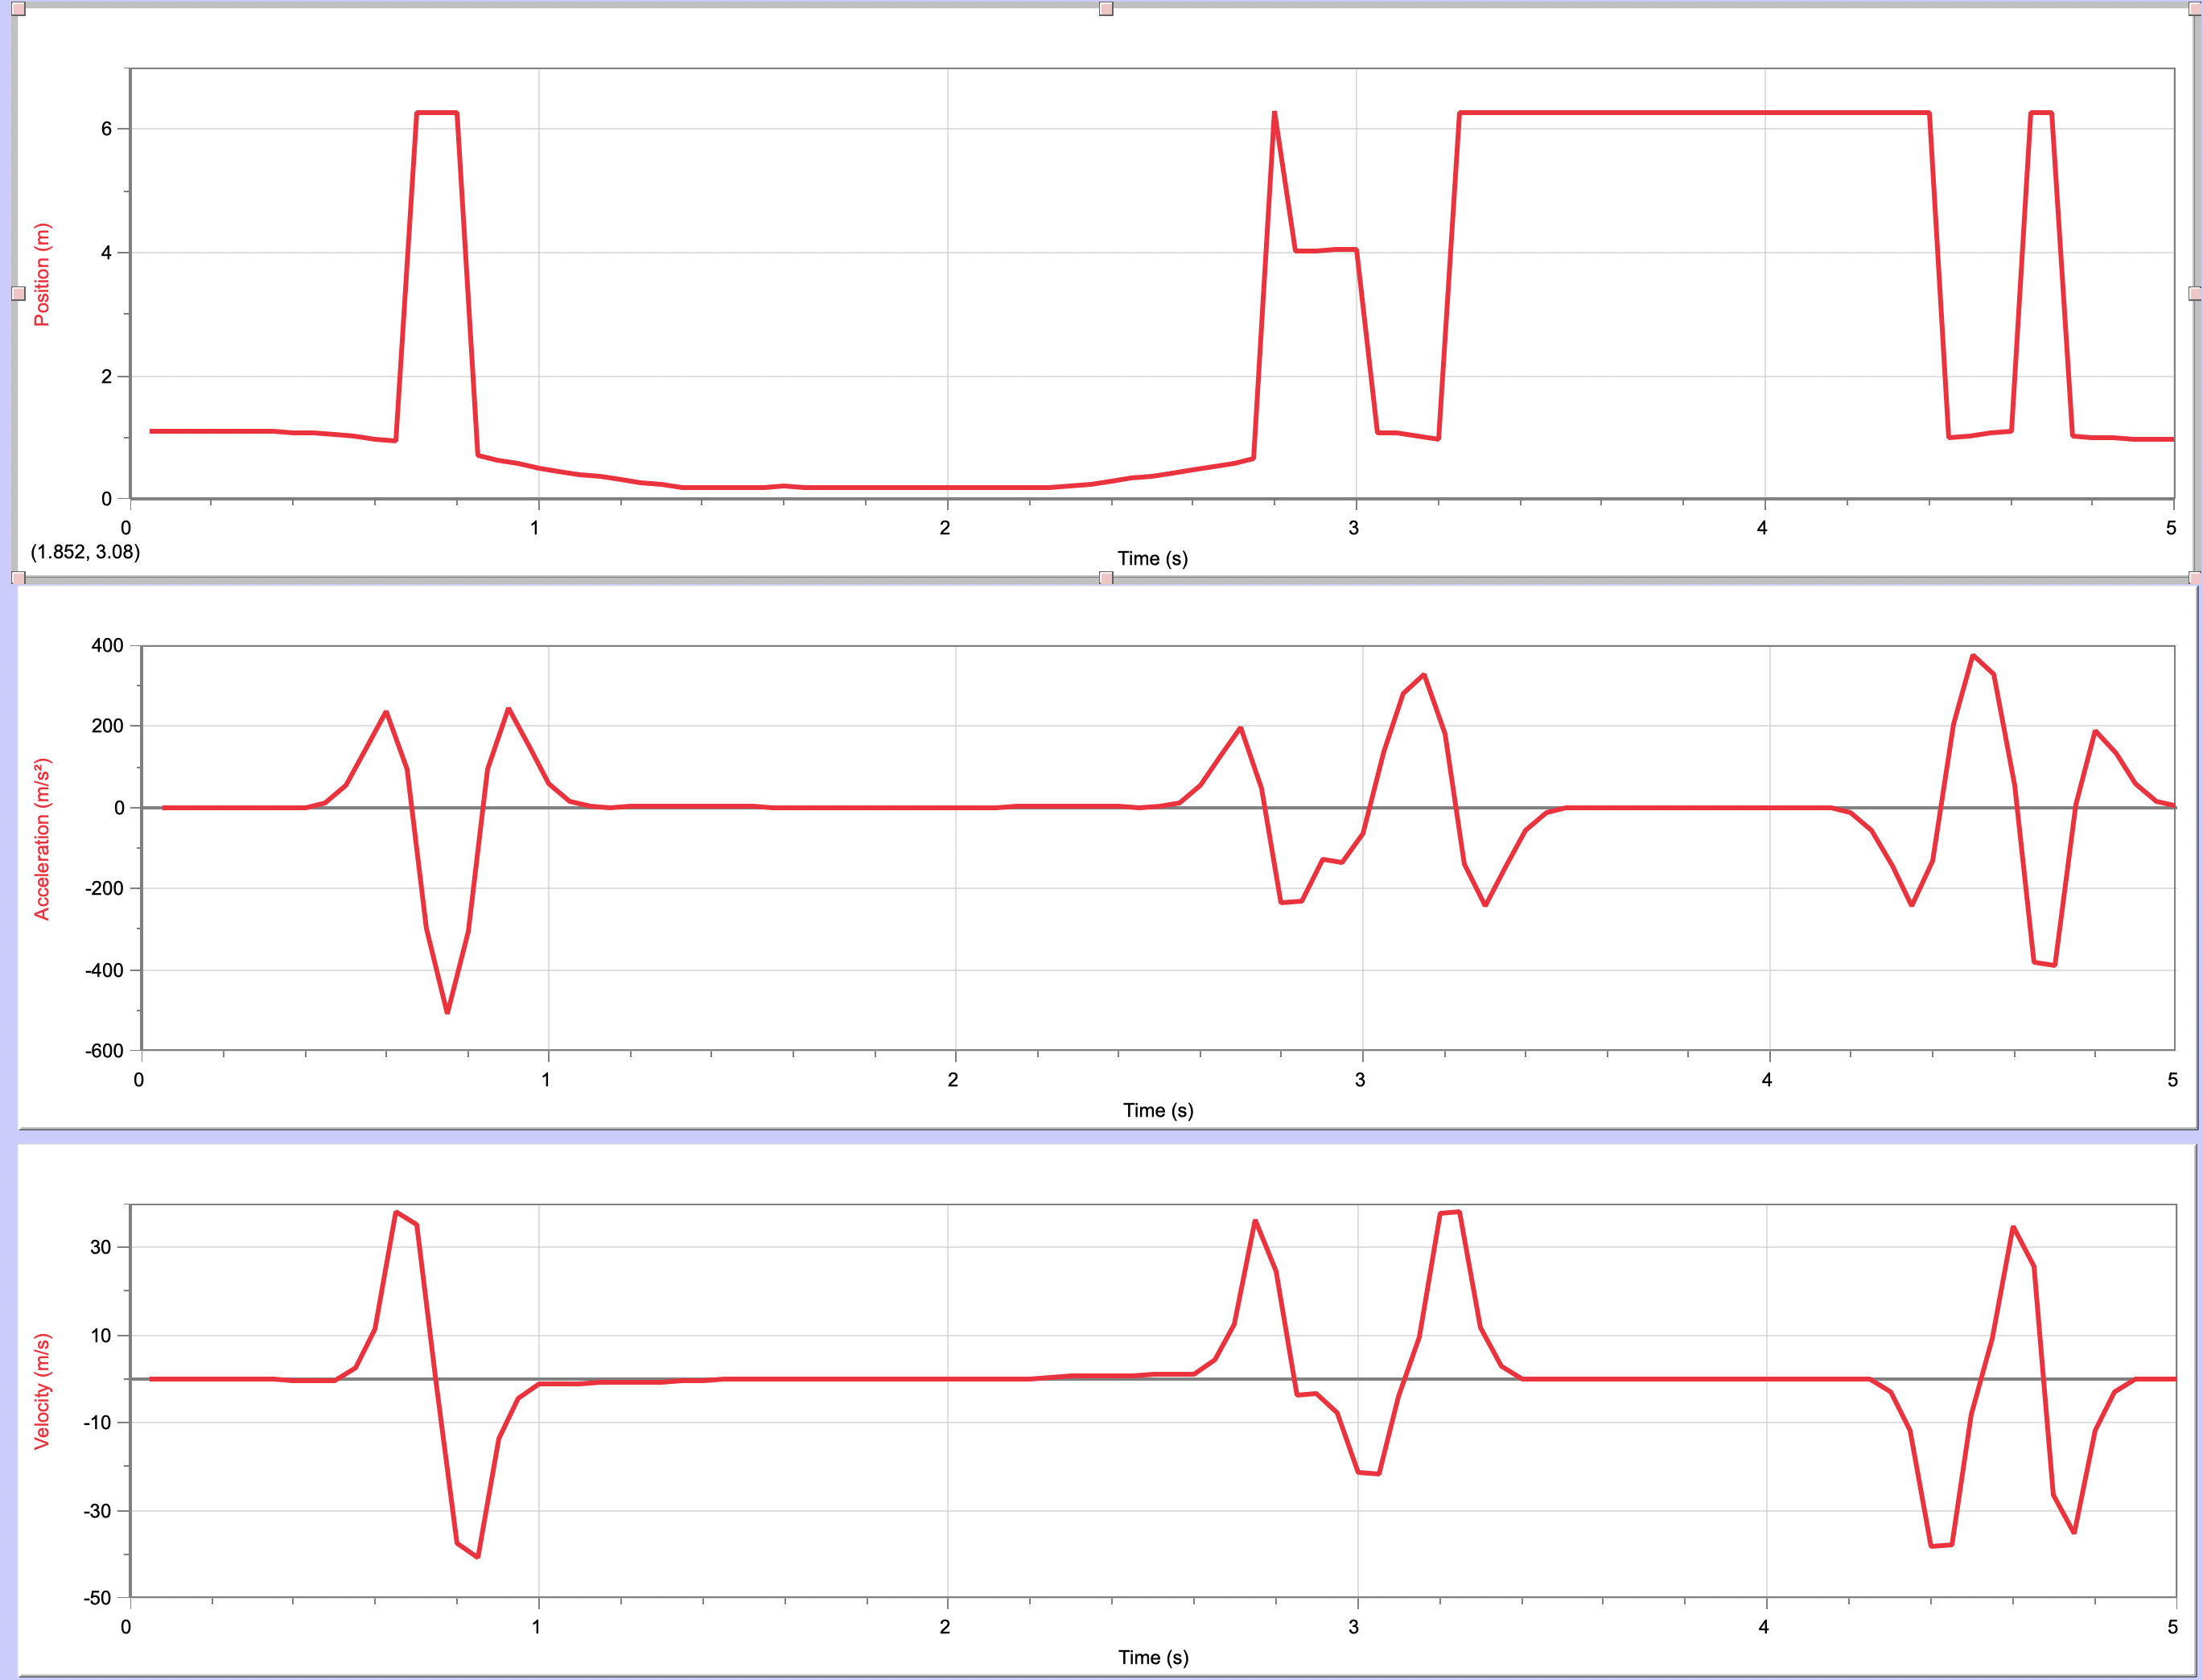
\includegraphics[width=1\linewidth]{images/Lab.02/PushUp1.png}
\end{center}
\caption{Run 1 of 3 from cart being pushed up from bottom to top of the track}
\label{fig:Data of Cart PushUp1}
\end{figure}

\begin{figure}[H] % Example of including images
\begin{center}
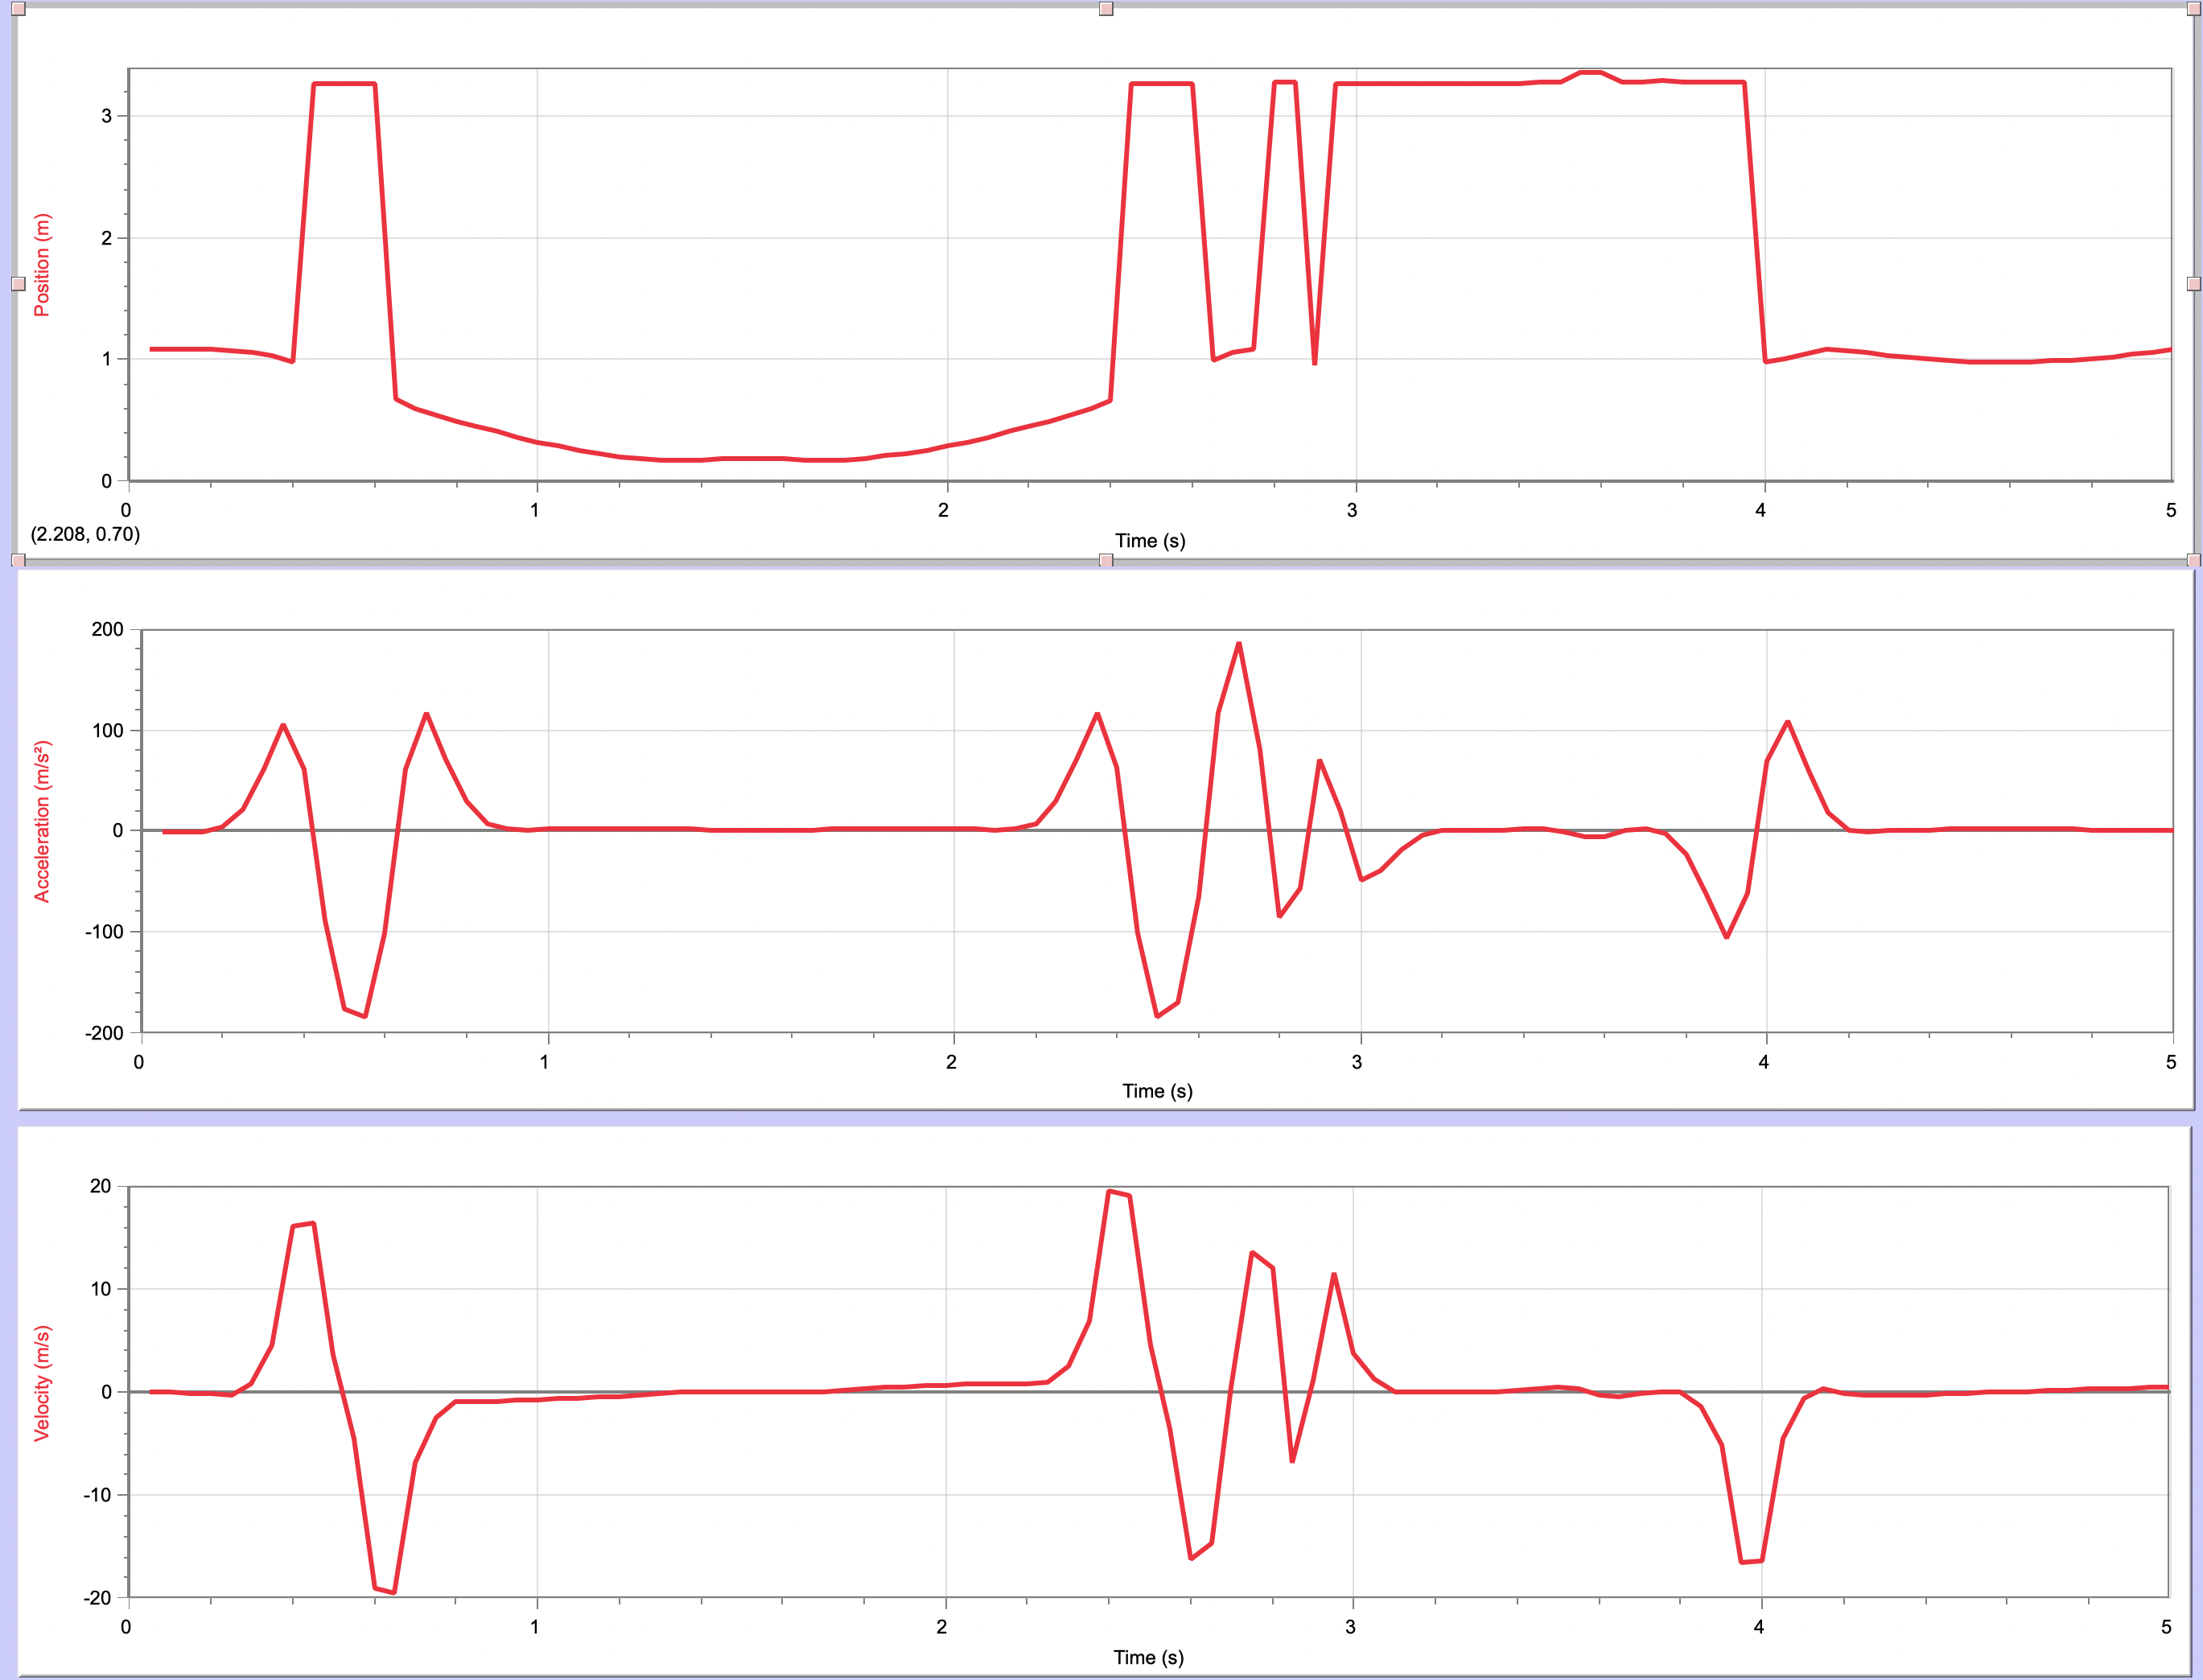
\includegraphics[width=1\linewidth]{images/Lab.02/PushUp2.png}
\end{center}
\caption{Run 2 of 3 from cart being pushed up from bottom to top of the track}
\label{fig:Data of Cart PushUp2}
\end{figure}

\begin{figure}[H] % Example of including images
\begin{center}
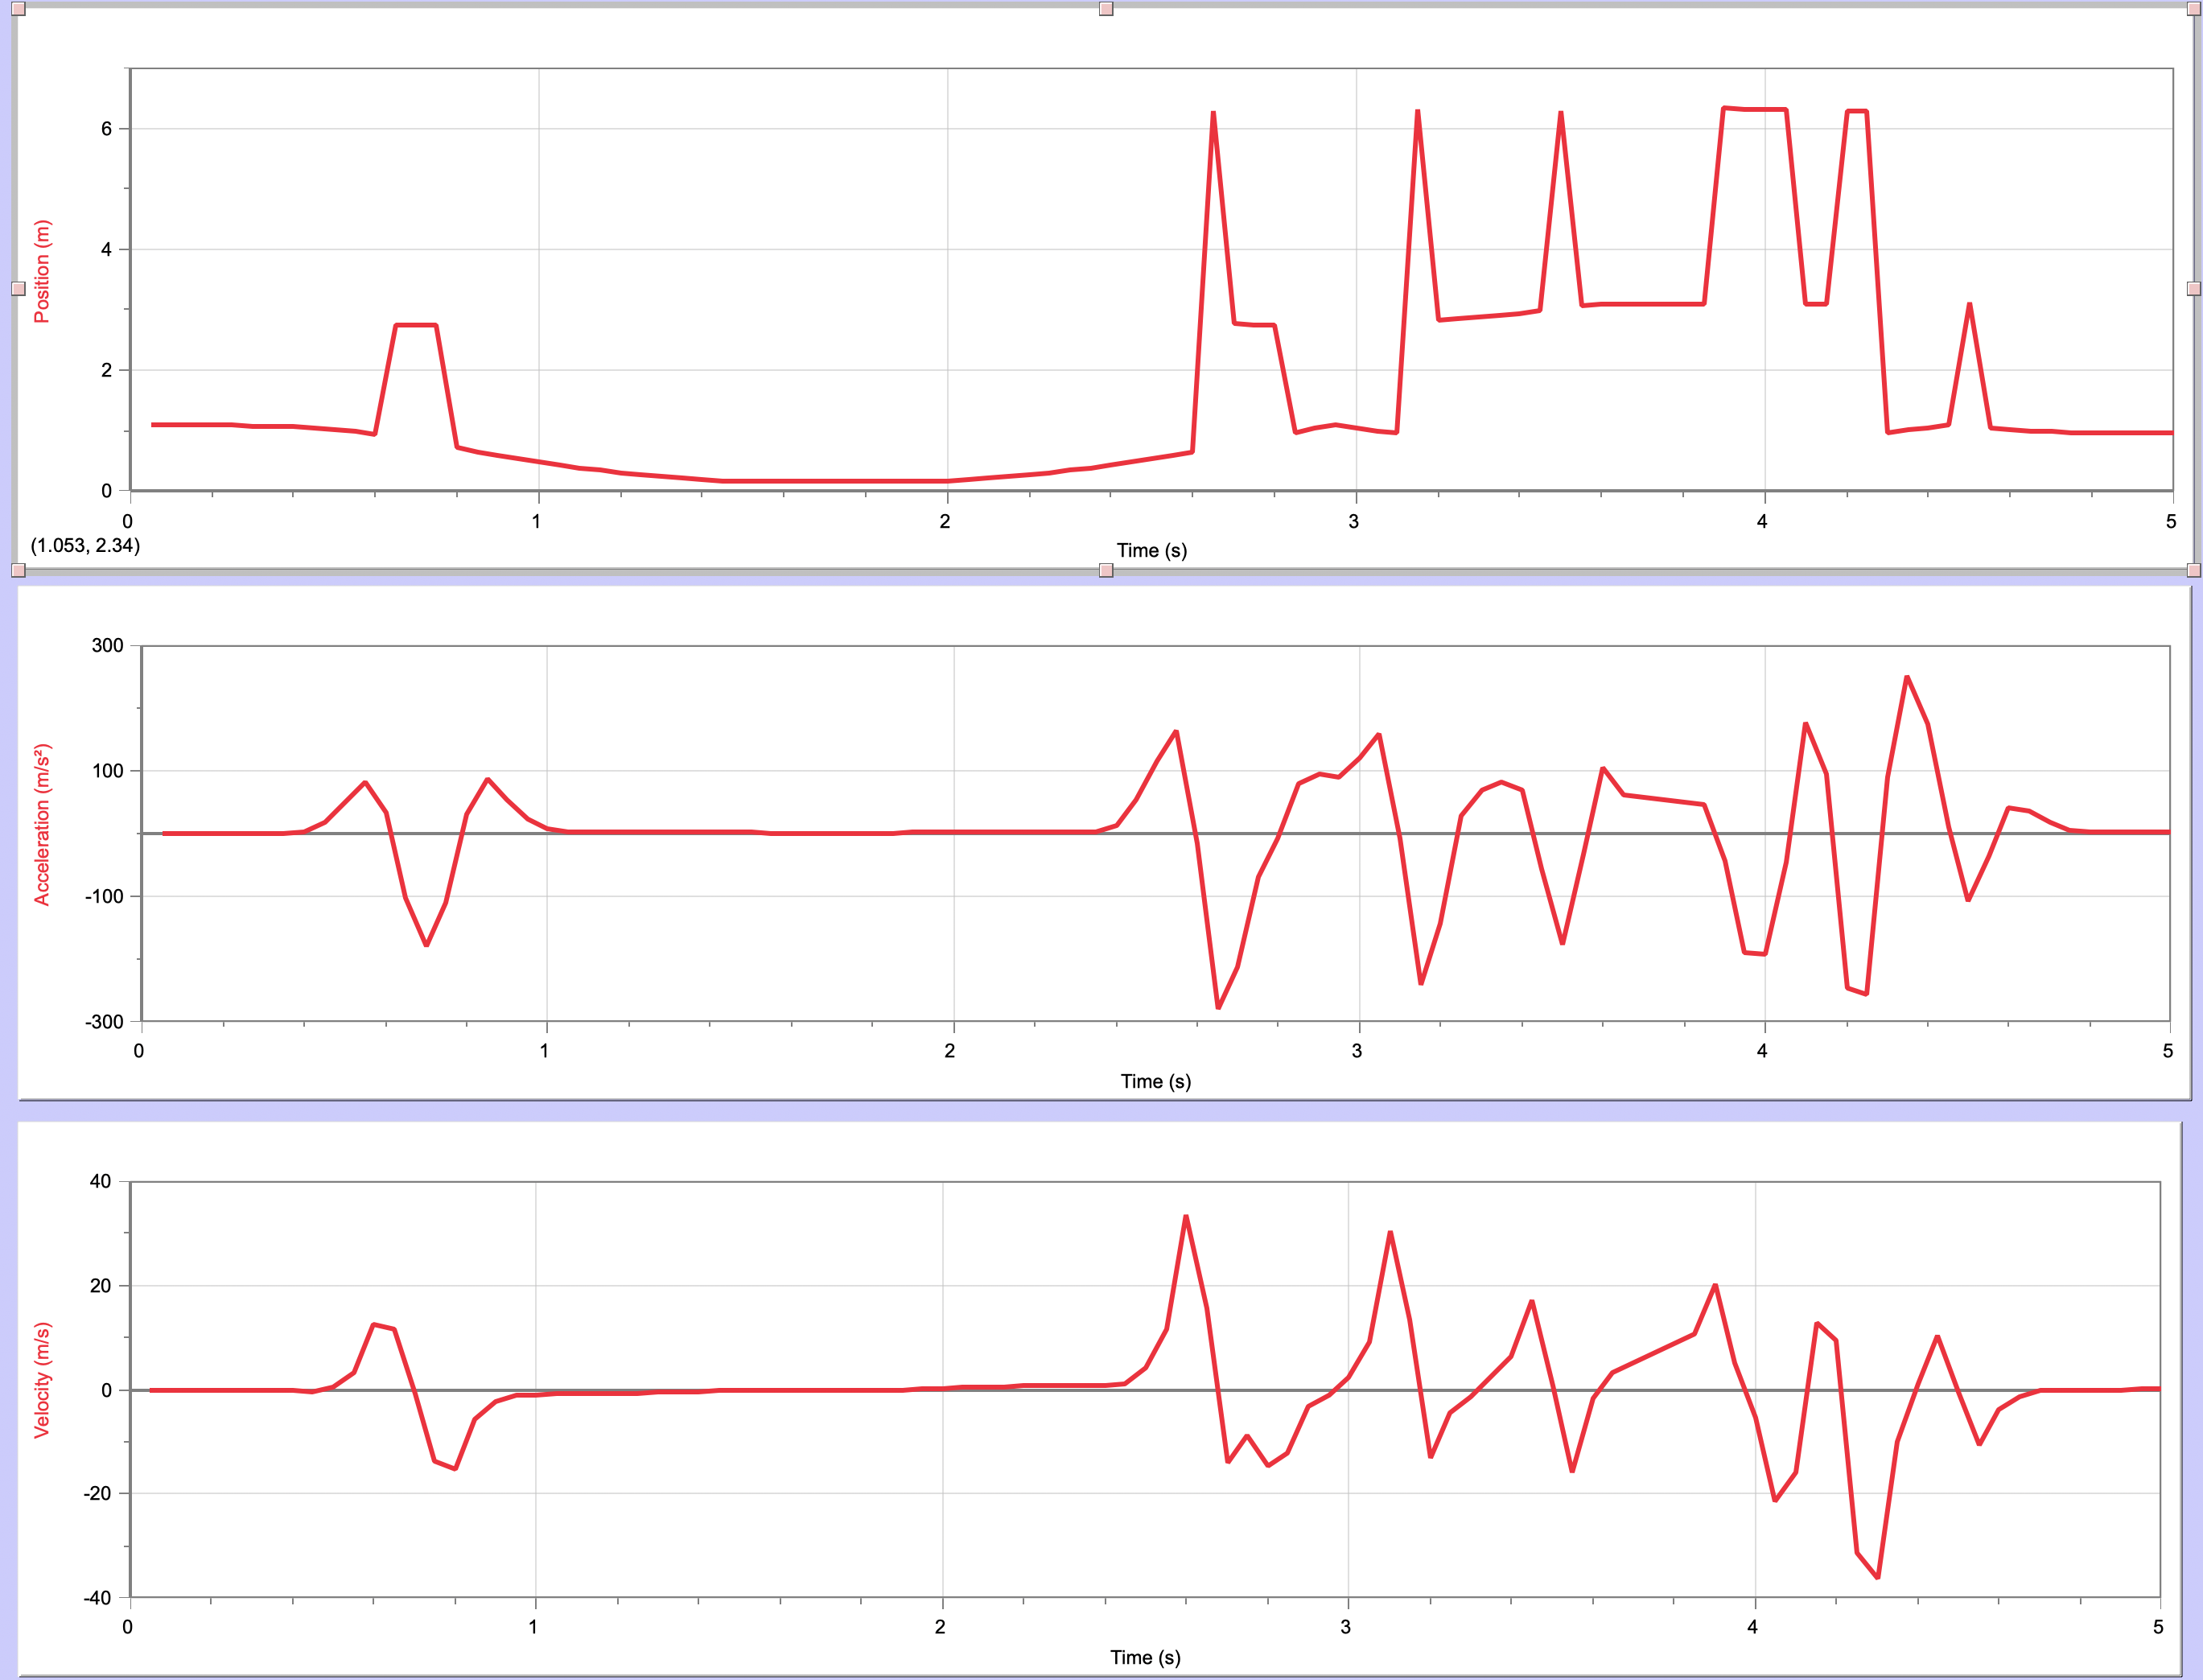
\includegraphics[width=1\linewidth]{images/Lab.02/PushUp3.png}
\end{center}
\caption{Run 3 of 3 from cart being pushed up from bottom to top of the track}
\label{fig:Data of Cart PushUp3}
\end{figure}

%----------------------------------------------------------------------------------------

\experiment{Lab Notebook Prompts}
\begin{enumerate}
    \item What are different ways to get the cart moving? Do the different ways affect it motion? If so, what do you consider an “optimal” way of moving the cart to observe constant acceleration as the cart moves up and down the track?
    \item How do you determine if you’ve gotten good quality data? What characteristics are you looking at? Why did you choose those characteristics?
    \item Figure out a way to show the cart moving in both directions on the inclined track it the same data collection event. Make sure to include a screenshot of the Logger Pro position, velocity, and acceleration graphs for a particularly “good” example of the data.
    \begin{enumerate}[(a)]
        \item Annotate the graphs to indicate the cart’s specific motions at different times any reasons when acceleration is not constant.
        \item Using the relationships between position, velocity, and acceleration, prove that you’ve collected data of the cart undergoing constant acceleration on an inclined track. Discuss the relationships between the position, velocity, and acceleration graphs in the context of the cart’s motion. What do you expect the relationships to be? Point out any differences between your expectations and the graphs.
    \end{enumerate}
\end{enumerate}

%----------------------------------------------------------------------------------------

\experiment{Lab Notebook Answers}
\begin{enumerate}
    \item There is more than one way to get the cart moving. For me, I pushed it to get it moving up the ramp, and for it to move down the ramp, I just put it at the top and let it go. I don't think the different ways affect the motion that much besides when it is being pushed because the speed will depend on how hard you push the cart. I think for me the most optimal way to move the cart is to let it fall from the top of the track to the bottom of the track.
    \item To determine if I have good quality data - if the data doesn't have any sudden fluctuations like my pictures. Usually, the data for this experiment should be smooth and isn't supposed to have any rectangles or data where it seems like it was somehow able to teleport really quickly. I chose these characteristics because, based on my data, it was way off when I compared my data to other people. My data shows that the cart teleported and traveled way too fast. This shouldn't be possible, so this was why I chose these characteristics.
    \item Answer to 3
    \begin{enumerate}[(a)]
        \item See Figures
        \item If my data was correct according to the cart and motion detector, then you would generally see that one of the relationships between the acceleration and velocity is that when the position has a spike, the velocity will also have a tiny spike. On the other hand, the acceleration will have a big spike, but it will be in the negative direction. These spikes can usually be attributed to when the cart is being stopped by your hand and when they are being pushed by your hand.
    \end{enumerate}
\end{enumerate}

%----------------------------------------------------------------------------------------

\labday{Wednesday, 14 February 2024}
\vspace{-5mm}
Tiffany Pham

\experiment{Lab 04 (Lab) - Local G}
\vspace{-5mm}
\hfill \break
\textbf{Purpose}
\begin{enumerate}
    \item Become familiar with lab equipment (Logger Pro, Track, Vernier).
    \item Gain experience collecting and analyzing real data and making reasoned, supported conclusions on what that data means.
    \item Practice recording what you're doing and why in your lab notebook.
    \item Answer the overall lab question on if "its it possible to detect the latitudinal effects of little g using the available lab equipment?"
\end{enumerate}

\hfill \break
\textbf{Predictions}

I predict that the lab equipment will be able to detect the latitudinal effects of little g with an offset of +-5.

\hfill \break
\textbf{Procedure}
\begin{enumerate}
    \item Turn on the computer or laptop and go to the Logger Pro application and start a new file/ experiment.
    \item Set up the track, cart, and motion detector if it isn't set up already. Make sure the magnets (grey end) face away from the motion detector, and do not let the cart crash into the motion detector.
    \item When increasing the angle of the track, make sure the legs at the bottom end are supporting it (rather than the metal tab that holds the bumper).
    \item If you let the cart bounce off the bumper at the far end of the track (away from the motion detector), make sure the cart stays in the track grooves. Have someone at the bumper end of the track to catch the cart, just in case.
    \item Start doing your multiple runs for your multiple angles. Change the angle after every couple runs or until you are satisfied for each of your angle runs. 
    \item Hold the cart at the top of the track. Once you press the collect button on Logger Pro, release the cart from the top and let it go down to record the data. Repeat steps until satisfied with experiment.
\end{enumerate}


\hfill \break 
What could go wrong:
\begin{itemize}
    \item Cart hitting the motion detector
    \item Cart falling off the track
    \item Not pushing it with enough force
    \item Motion detector not being angled correctly
\end{itemize}

\hfill \break
\textbf{Equipment needed}
\begin{itemize}
    \item Computer/ Laptop
    \item Logger Pro
    \item Vernier
    \item Motion Detector
    \item Track
    \item Cart
\end{itemize}

%----------------------------------------------------------------------------------------

\newpage
\experiment{Cart Data}
\begin{figure}[H] % Example of including images
\begin{center}
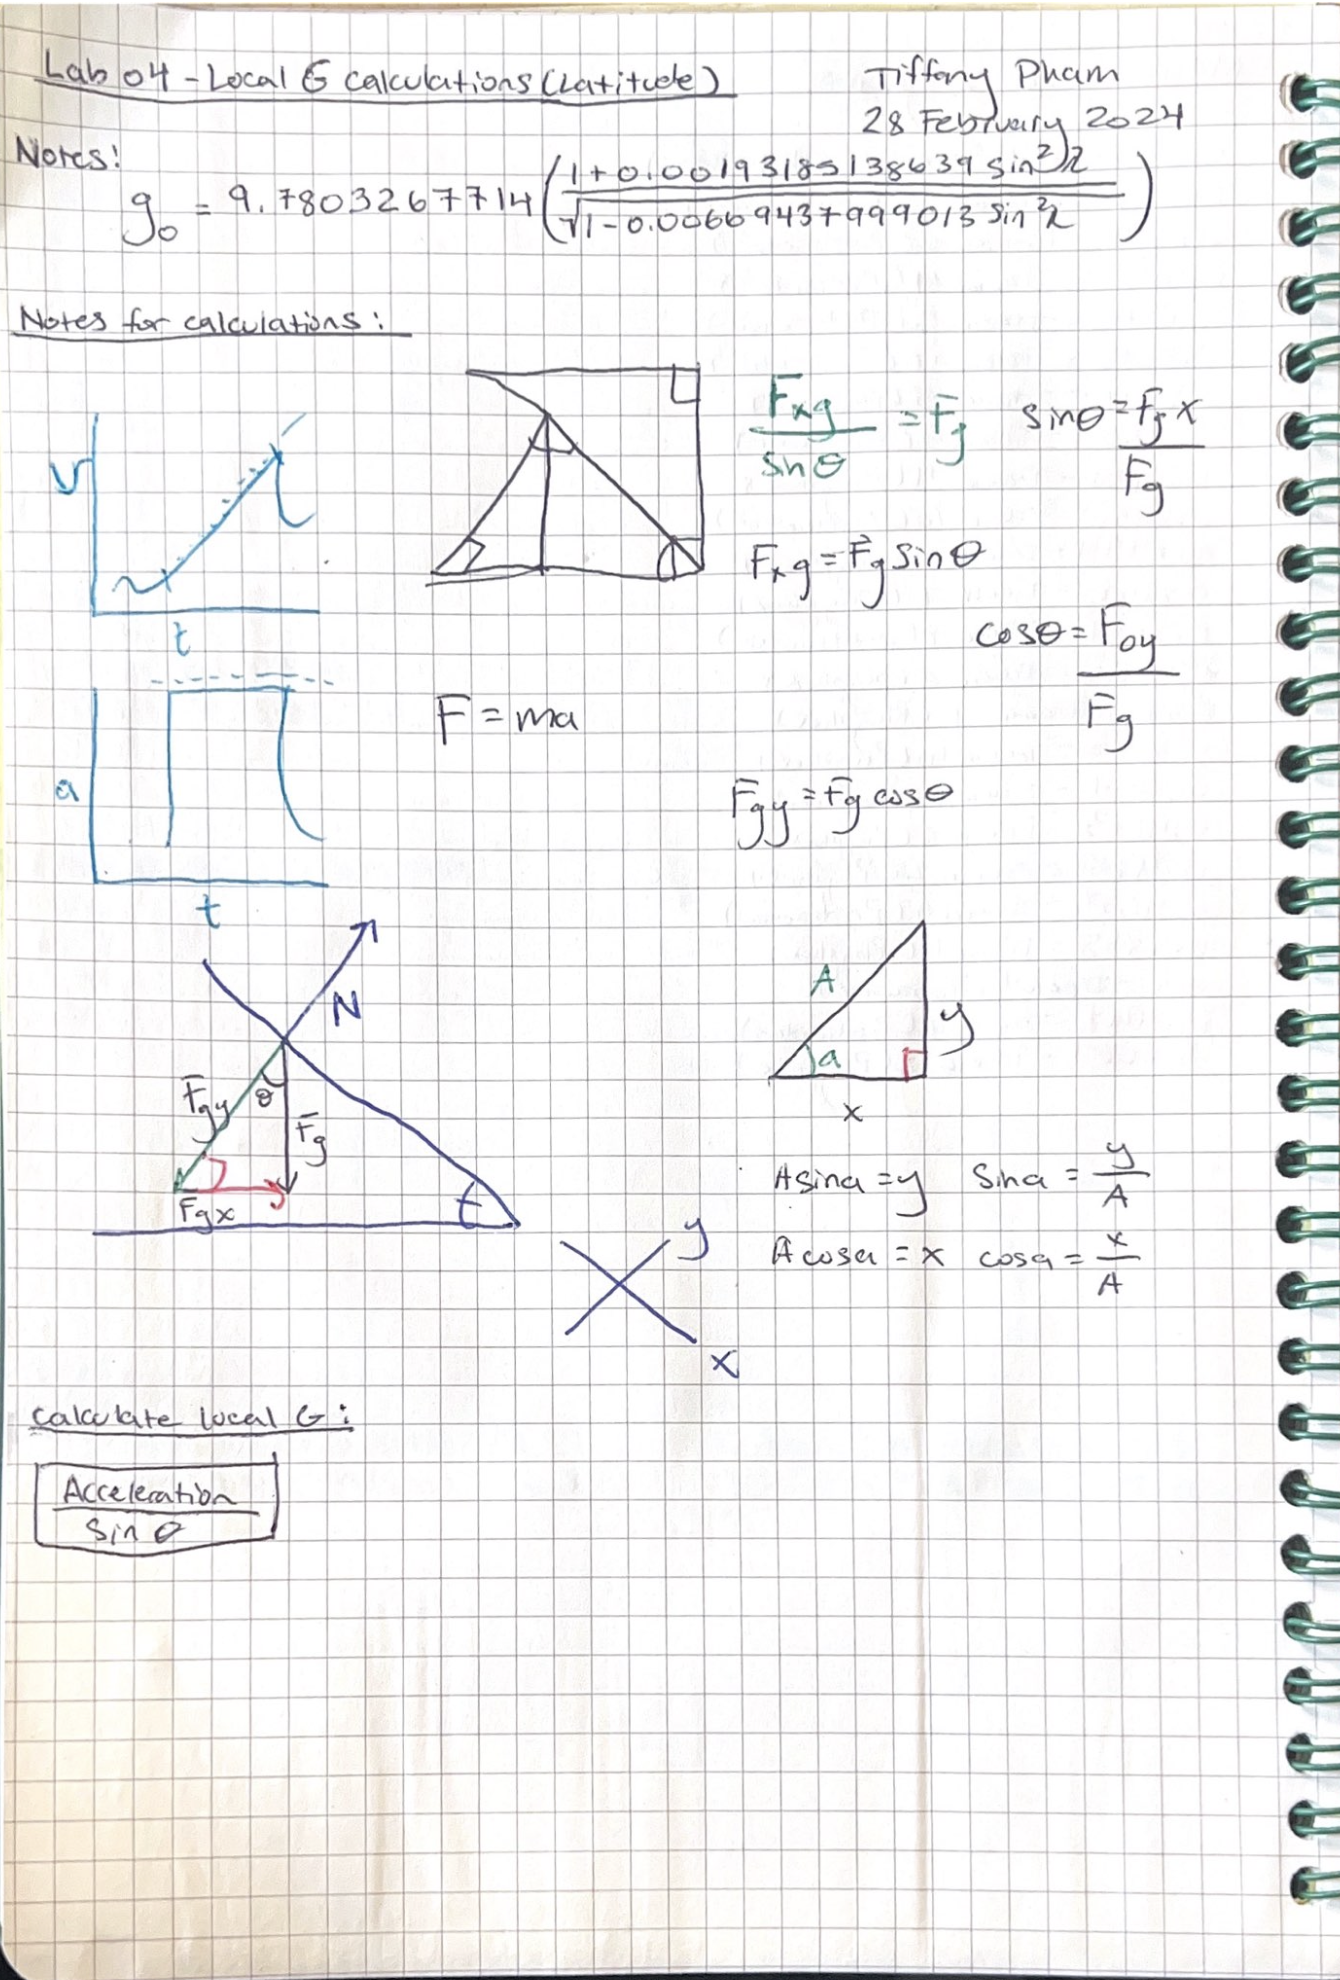
\includegraphics[width=0.8\linewidth]{images/Lab.04/LocalGCalculations1.png}
\end{center}
\caption{Calculation Notes for Local G}
\label{fig:Local G Calculations1}
\end{figure}

\begin{figure}[H] % Example of including images
\begin{center}
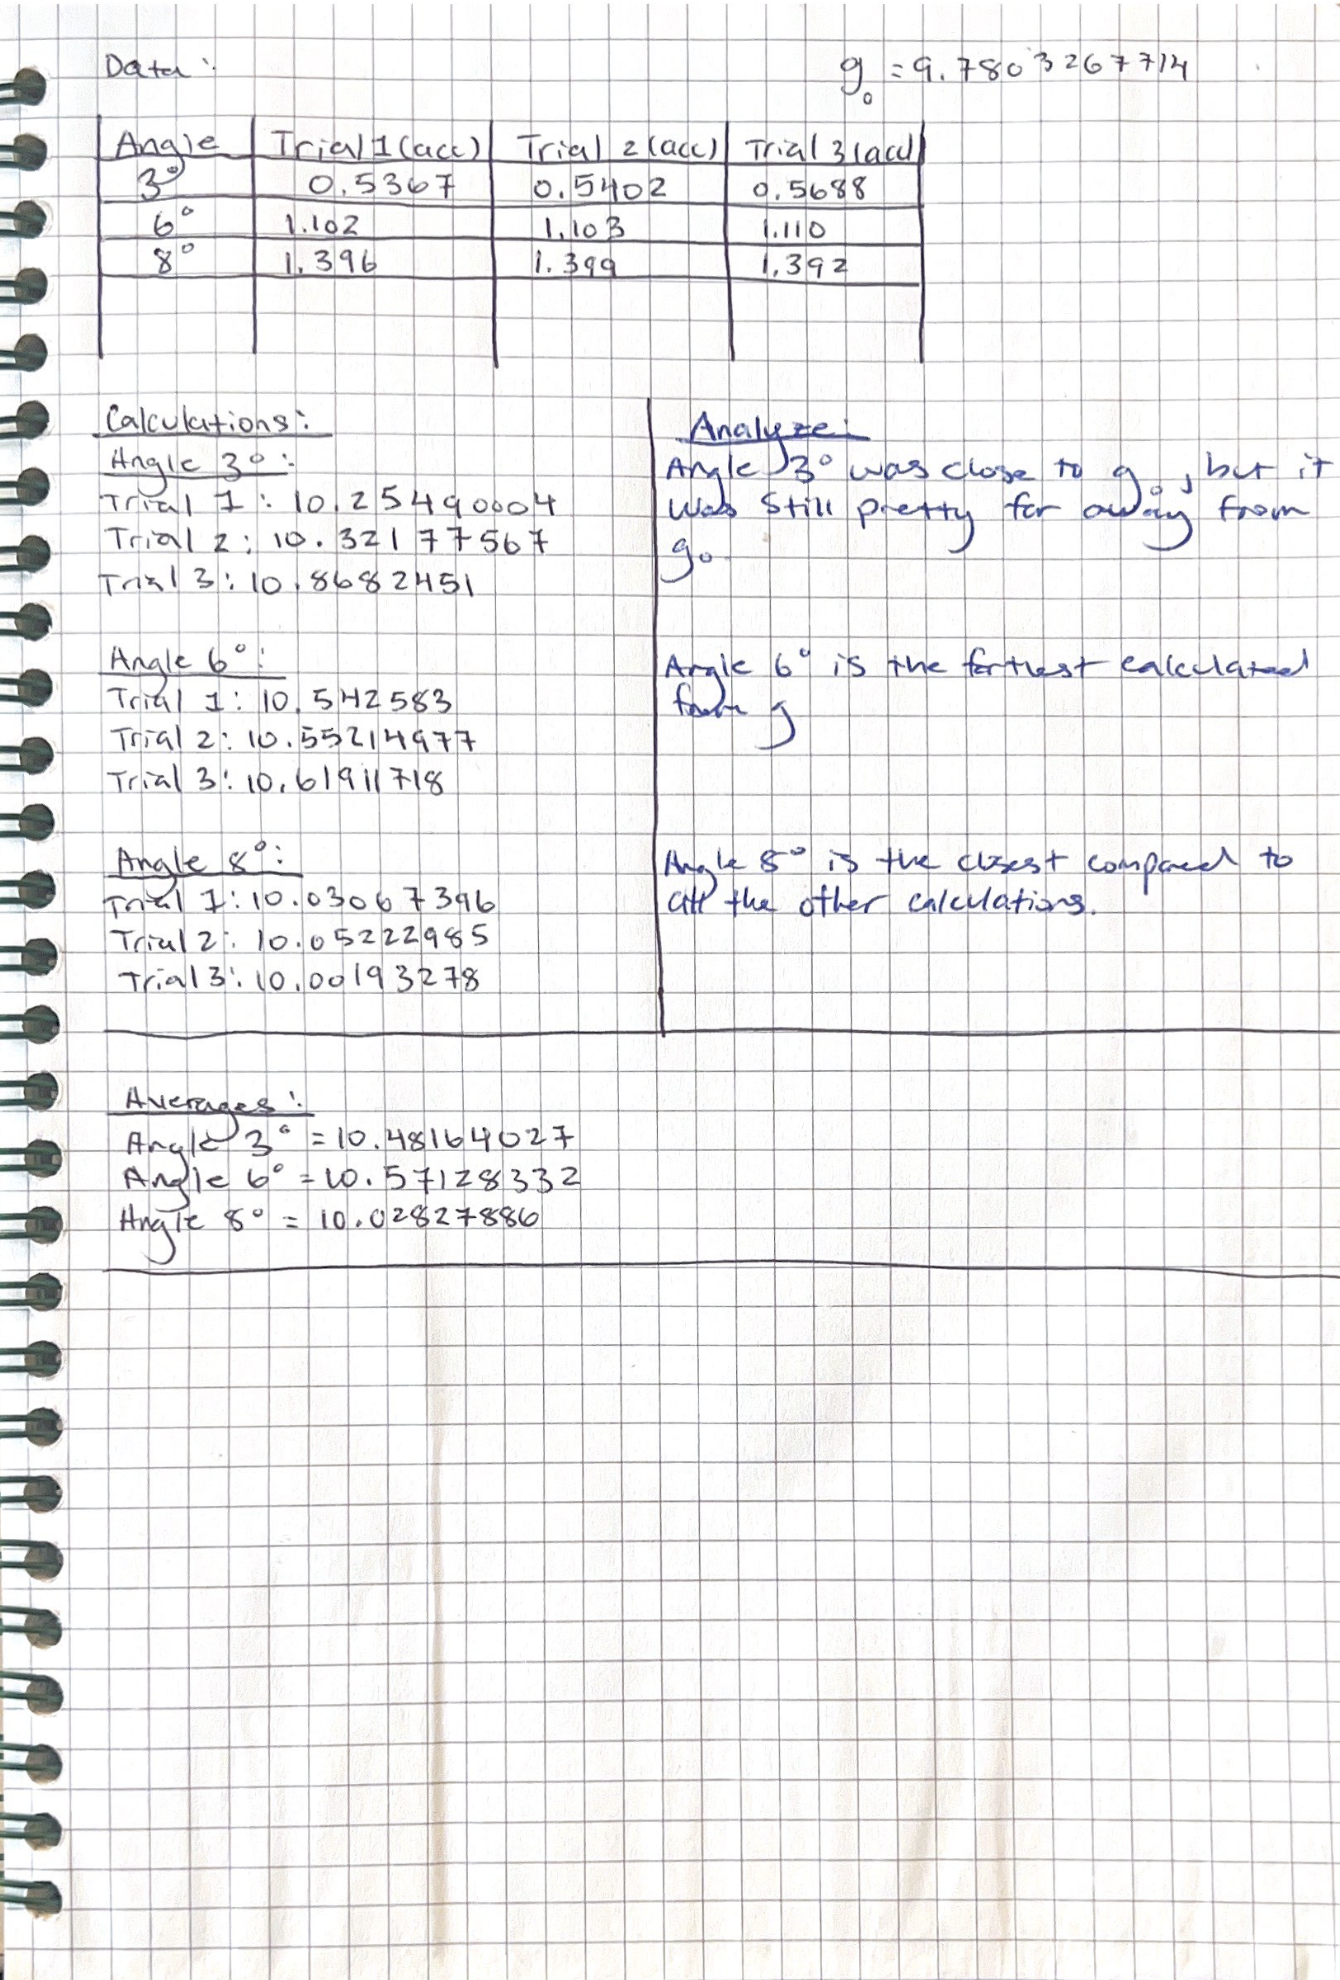
\includegraphics[width=1\linewidth]{images/Lab.04/LocalGCalculations2.png}
\end{center}
\caption{Calculations for all runs}
\label{fig:Local G Calculations2}
\end{figure}

%----------------------------------------------------------------------------------------

\experiment{Lab Notebook Prompts}
\begin{enumerate}
    \item \textbf{Overall Lab Question:} Is it possible to detect the latitudinal effects of little g using the available lab equipment?
\end{enumerate}

%----------------------------------------------------------------------------------------

\experiment{Lab Notebook Answers}
\begin{enumerate}
    \item Yes, it is sort of possible, but it'll be +-1 to +- 2 off.
\end{enumerate}

%----------------------------------------------------------------------------------------

\labday{Wednesday, 13 March 2024}
\vspace{-5mm}
Tiffany Pham

\experiment{Lab 05 (Lab) - Force Sensor}
\textbf{Purpose}
\begin{enumerate}
    \item Use your lab notebook to document your work and reasoning; referring to the lab notebook guidelines as needed.
    \item Correctly zero the Vernier dual-range force sensor.
    \item Measure forces using the Vernier dual-range force sensor.
    \item Determine which sensor attachments to use and ranges to use for accurate, reproducible force measurements in various ways with the provided materials.
\end{enumerate}

\hfill \break
\textbf{Objective}

Use the force sensor with different sensor attachments to determine which attachments and ranges to use for accurate, reproducible force measurements in various ways with the provided materials.

\hfill \break
\textbf{Predictions}

I predict that the force sensor will be able to accurately measure the force that is being acted upon itself.

\hfill \break
\textbf{Procedure}
\begin{enumerate}
    \item Turn on the computer or laptop and go to the Logger Pro application.
    \item Set up the track, cart, and force sensor alongside with all the other needed attachments if it isn't set up already.
    \item Pick the different attachments to use for the sensor (hook, bumper, thumb screw, handle).
    \item Pick what measurements to use (weights, string on weights, pushing the weights, etc.
    \item If you are using the track angle, when increasing the angle of the track, make sure the legs at the bottom end are supporting it (rather than the metal tab that holds the bumper).
    \item Once you're done with an attachment and measurement style, switch it around to see how many different forces you can create for the force sensor to measure.
\end{enumerate}

\hfill \break
What could go wrong:
\begin{itemize}
    \item The force sensor having false readings
\end{itemize}

\hfill \break
\textbf{Equipment needed}
\begin{itemize}
    \item Computer/ Laptop
    \item Logger Pro
    \item Vernier
    \item Force sensor
    \item Track
    \item Cart
    \item Attachments (hook, bumper, thumb screw, handle
    \item Forces (weights, string, etc)
\end{itemize}

%----------------------------------------------------------------------------------------

\newpage
\hfill \break
\experiment{Force Data}
\begin{figure}[H] % Example of including images
\begin{center}
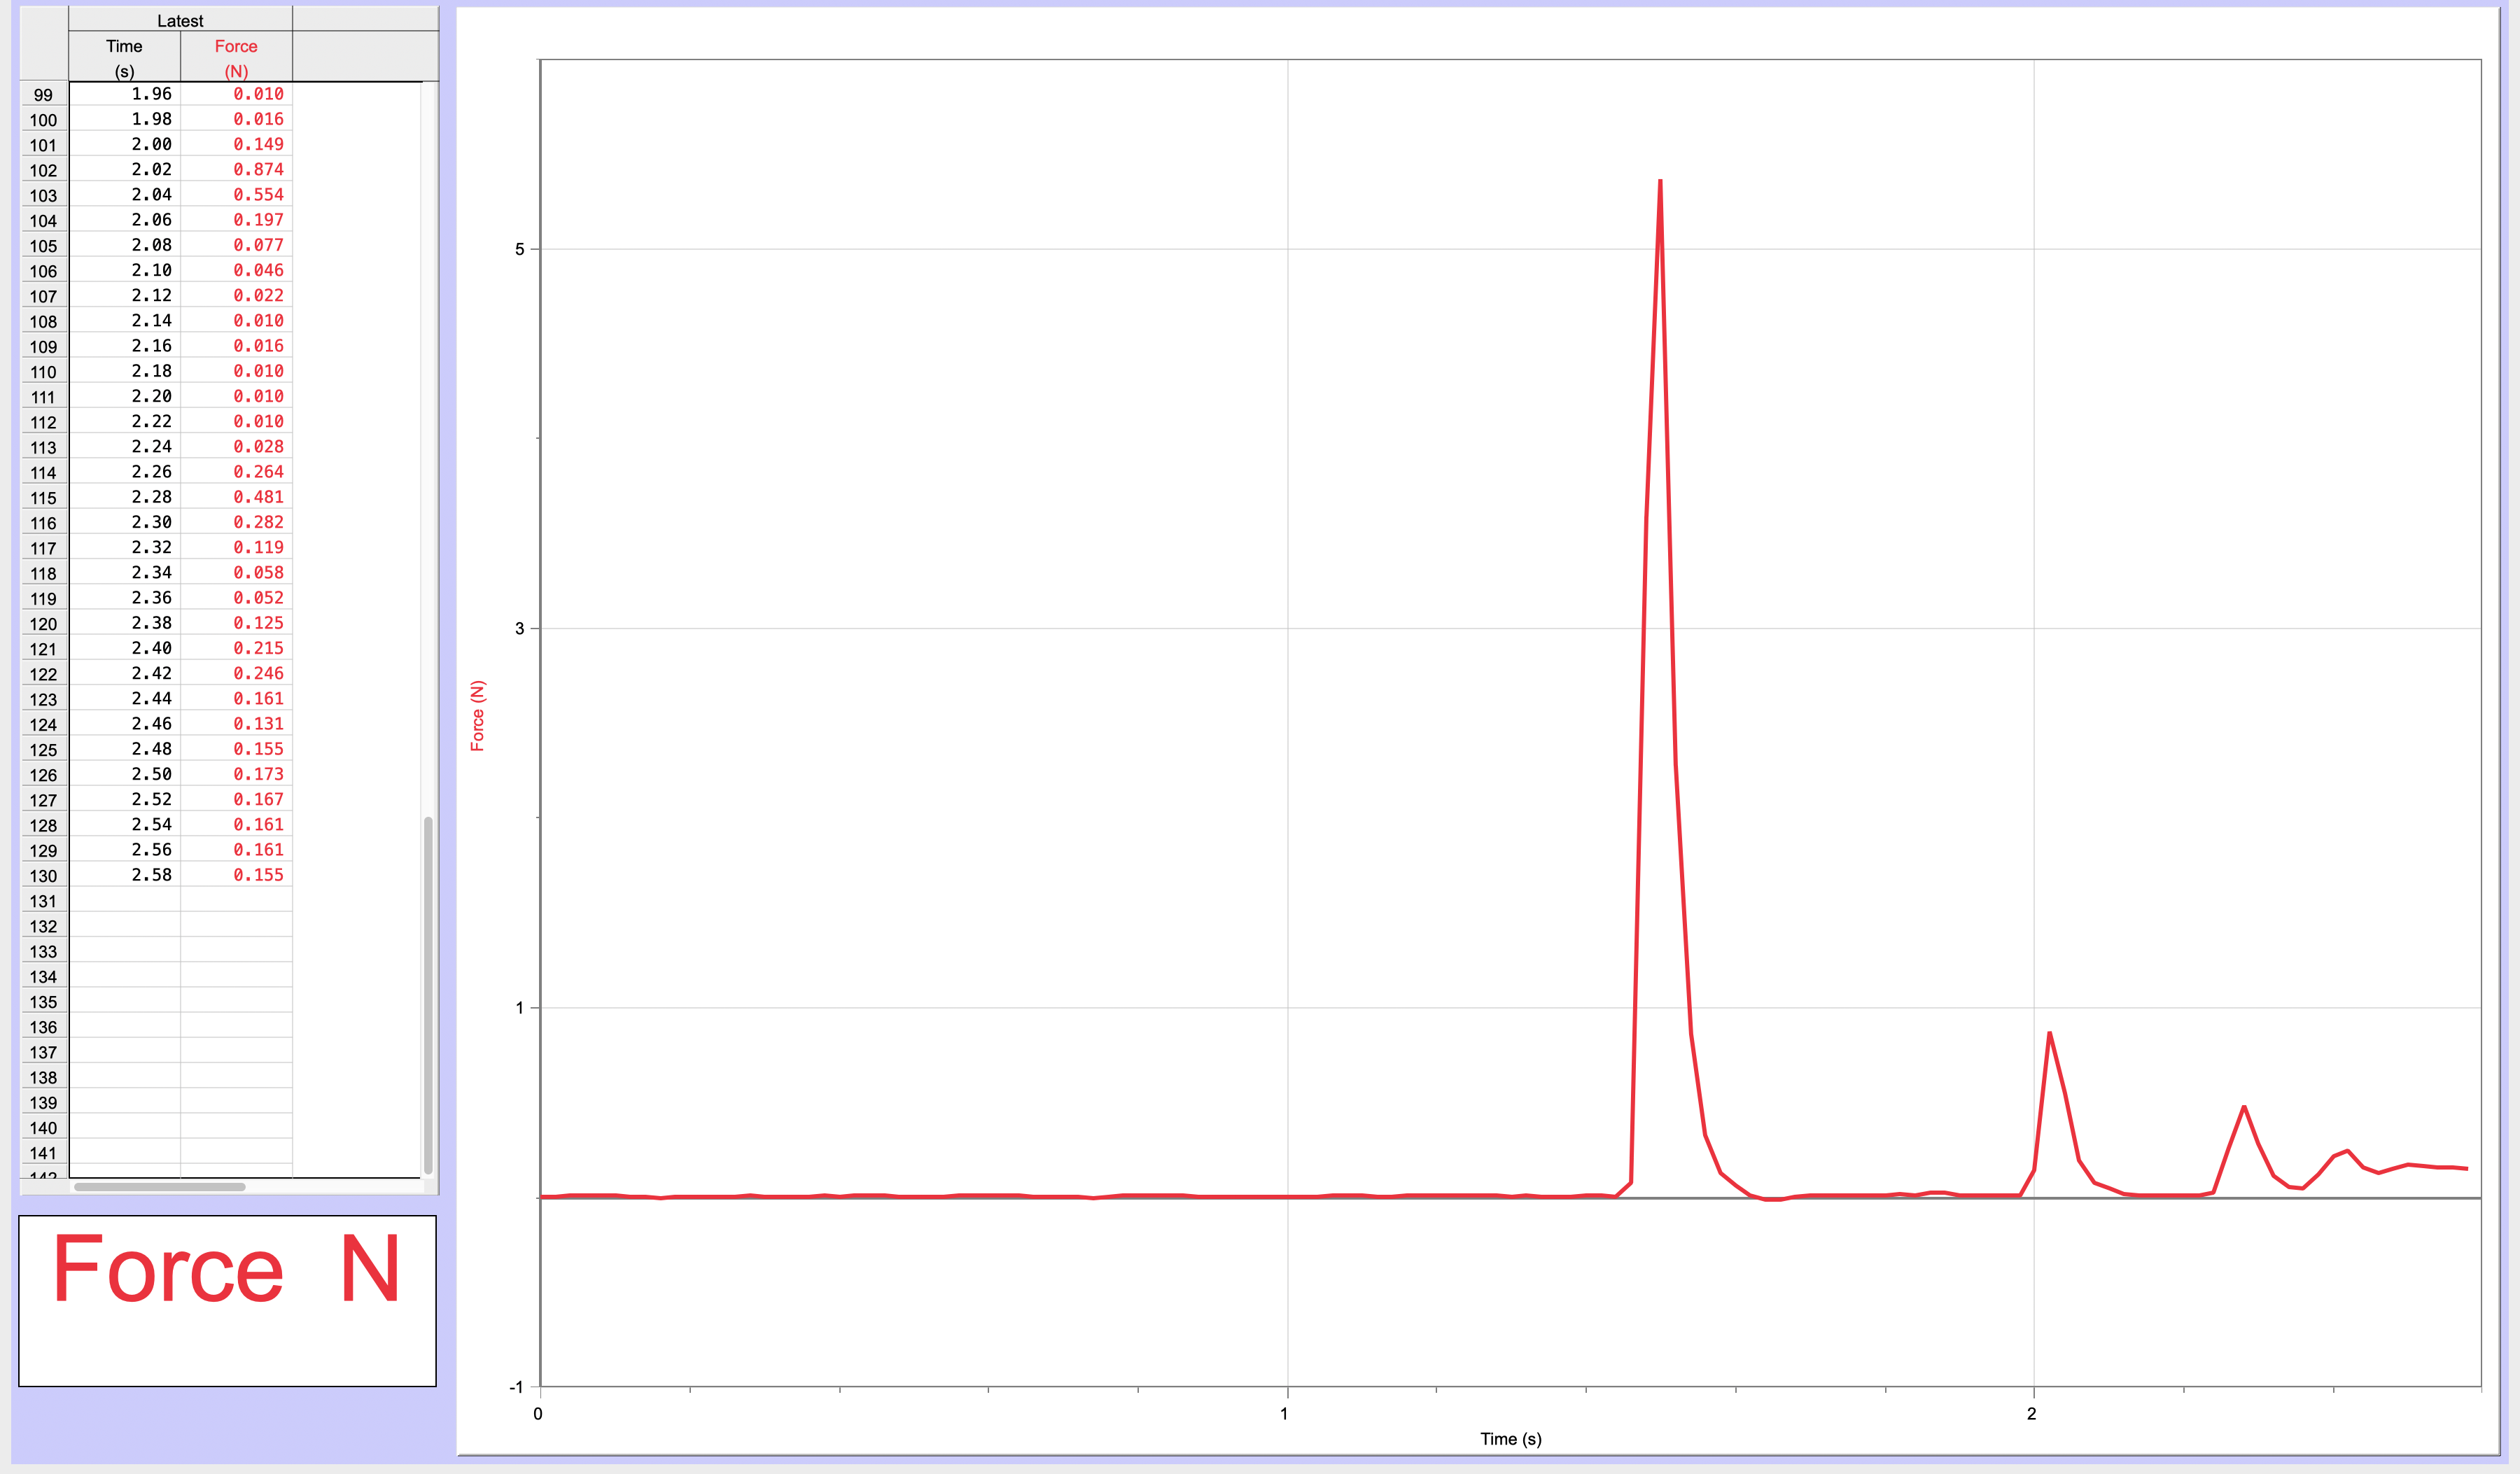
\includegraphics[width=1\linewidth]{images/Lab.05/Lab05.Run2.png}
\end{center}
\caption{Run 2 of 6. This run, the force sensor was mounted on the stand at \textbf{1.65 degrees} \textbf{horizontally} using the \textbf{thumb screw}. It was attached using the \textbf{hook} to a string to the \textbf{cart}, and we measured a \textbf{constant non-zero force}.}
\label{fig:Lab05-Run2}
\end{figure}

\begin{figure}[H] % Example of including images
\begin{center}
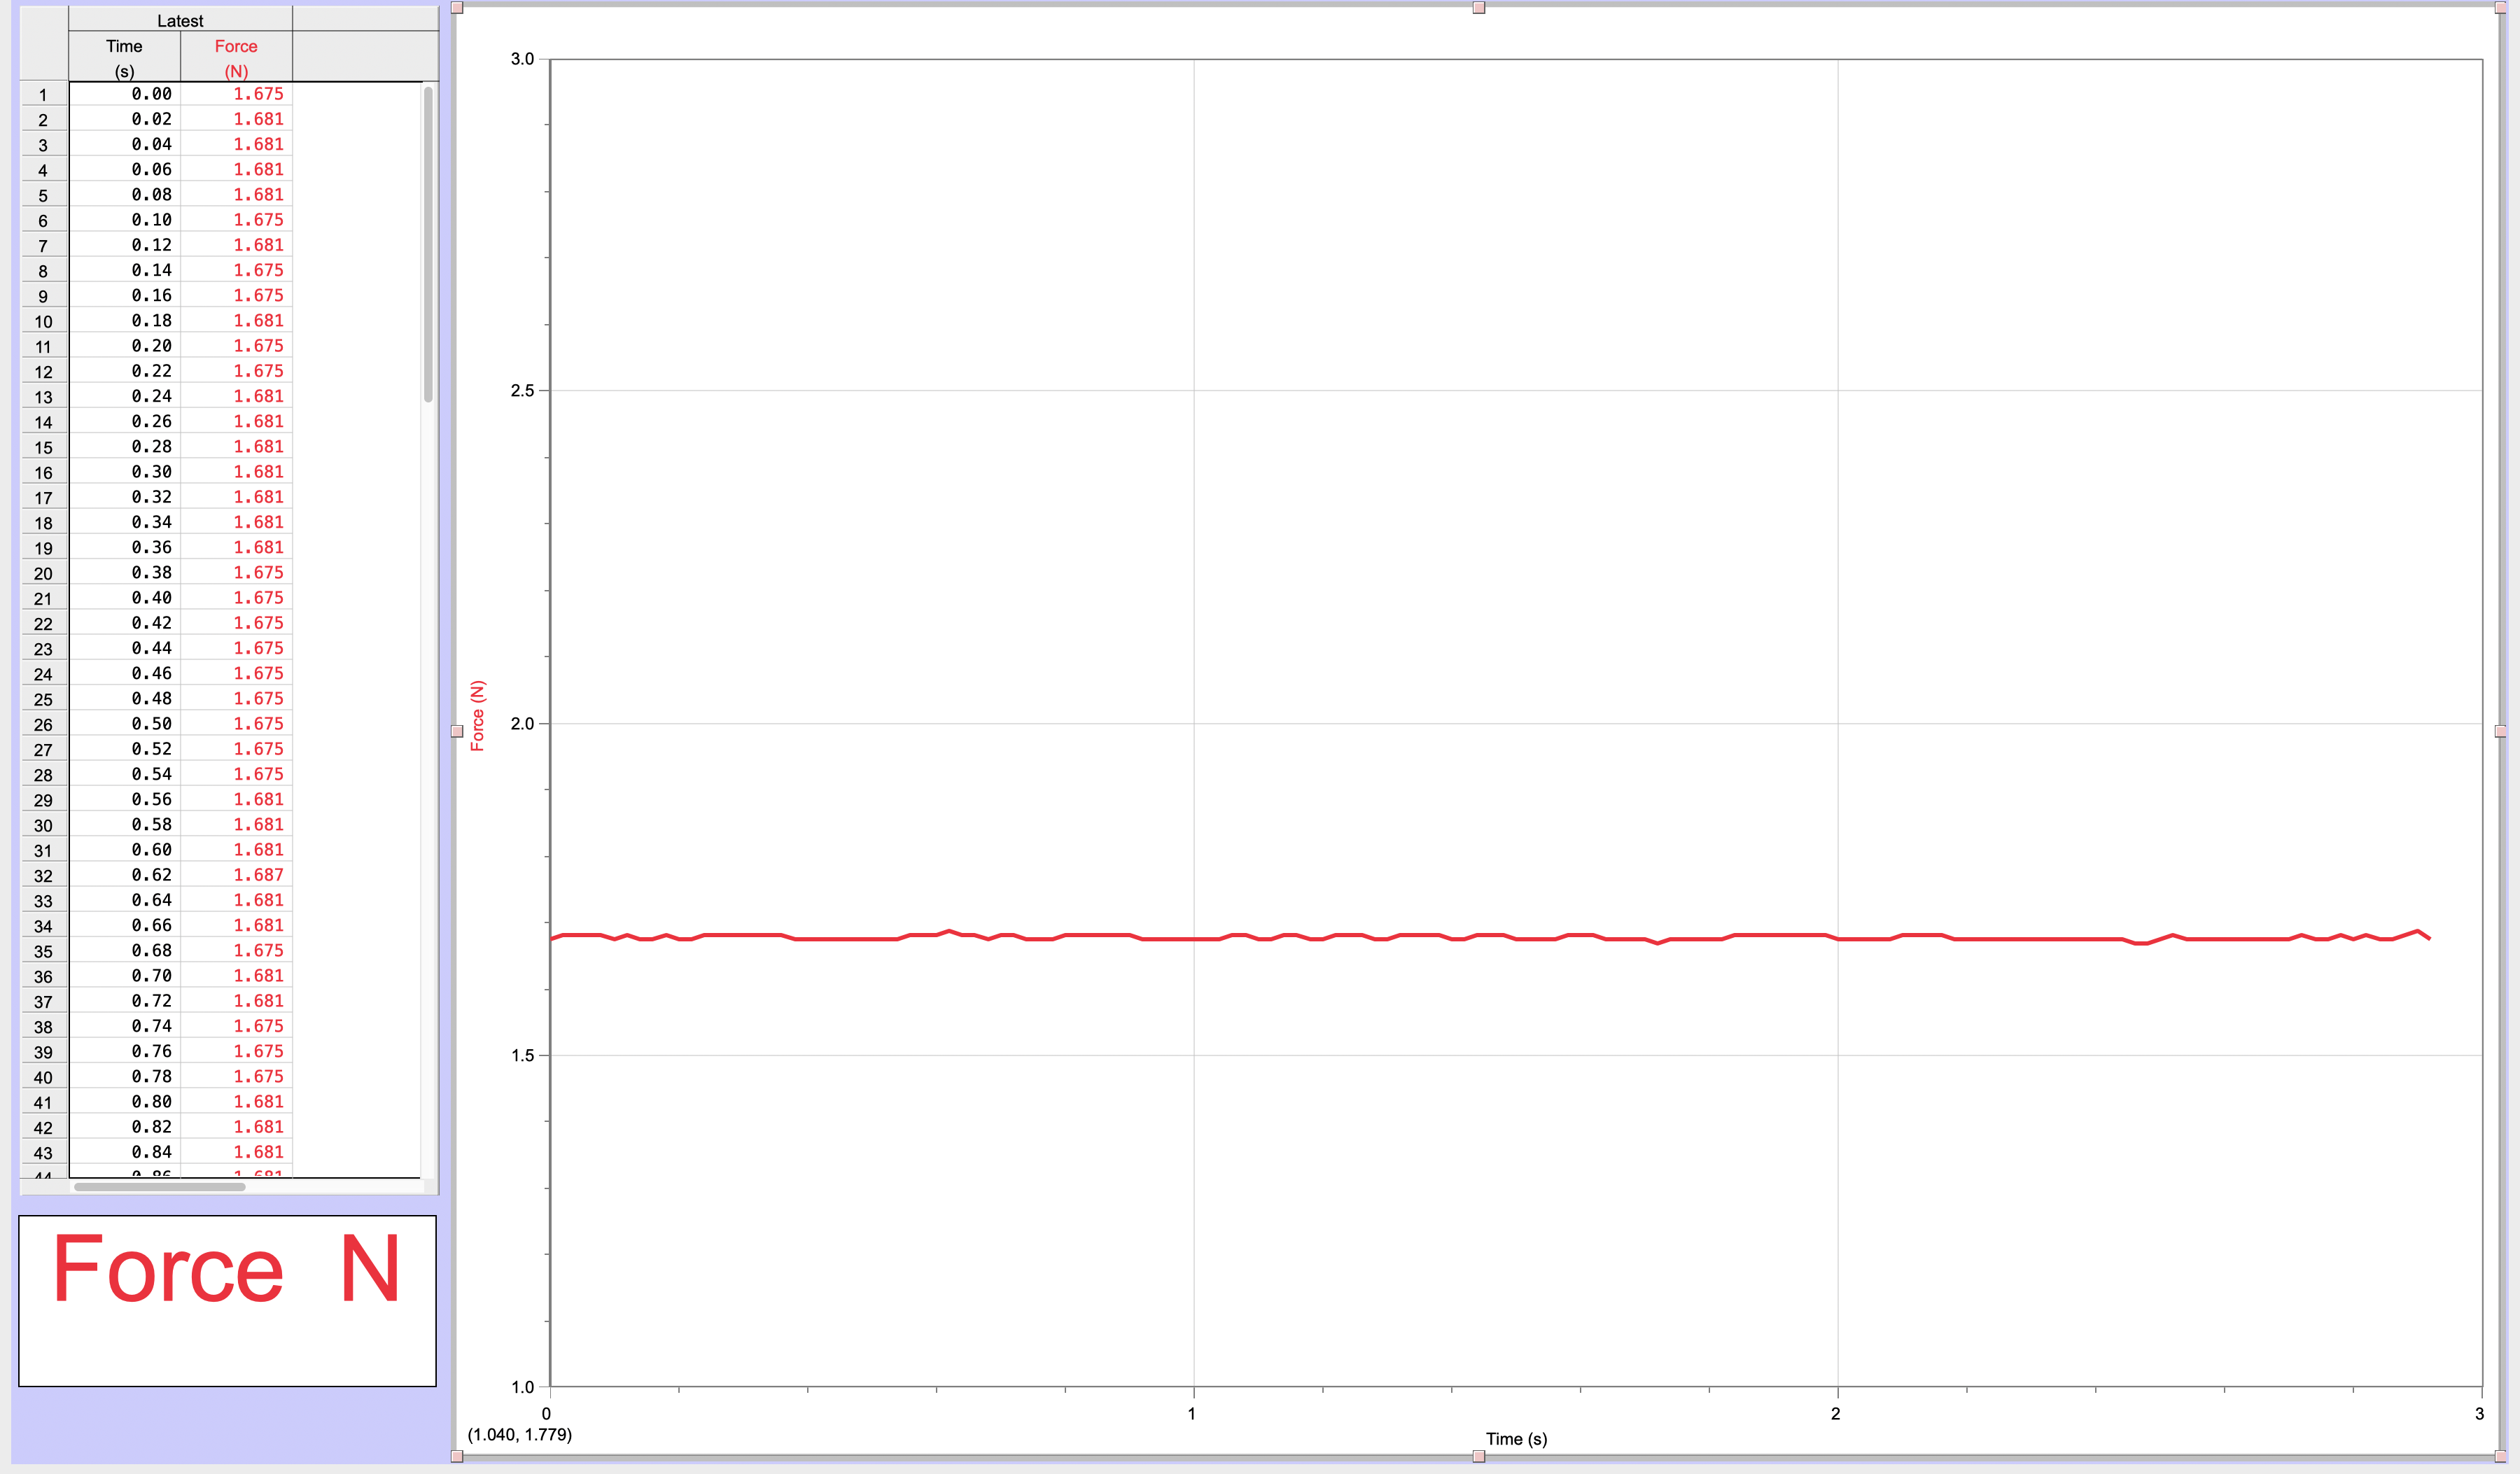
\includegraphics[width=.90\linewidth]{images/Lab.05/Lab05.Run3.png}
\end{center}
\caption{Run 3 of 6. This run, the force sensor was mounted on the stand \textbf{vertically} using the \textbf{thumb screw} and the \textbf{handle}. Using the \textbf{hook}, we attached \textbf{weights} to it (\textbf{170GM}) and measured a \textbf{constant force}.}
\label{fig:Lab05-Run3}
\end{figure}

\begin{figure}[H] % Example of including images
\begin{center}
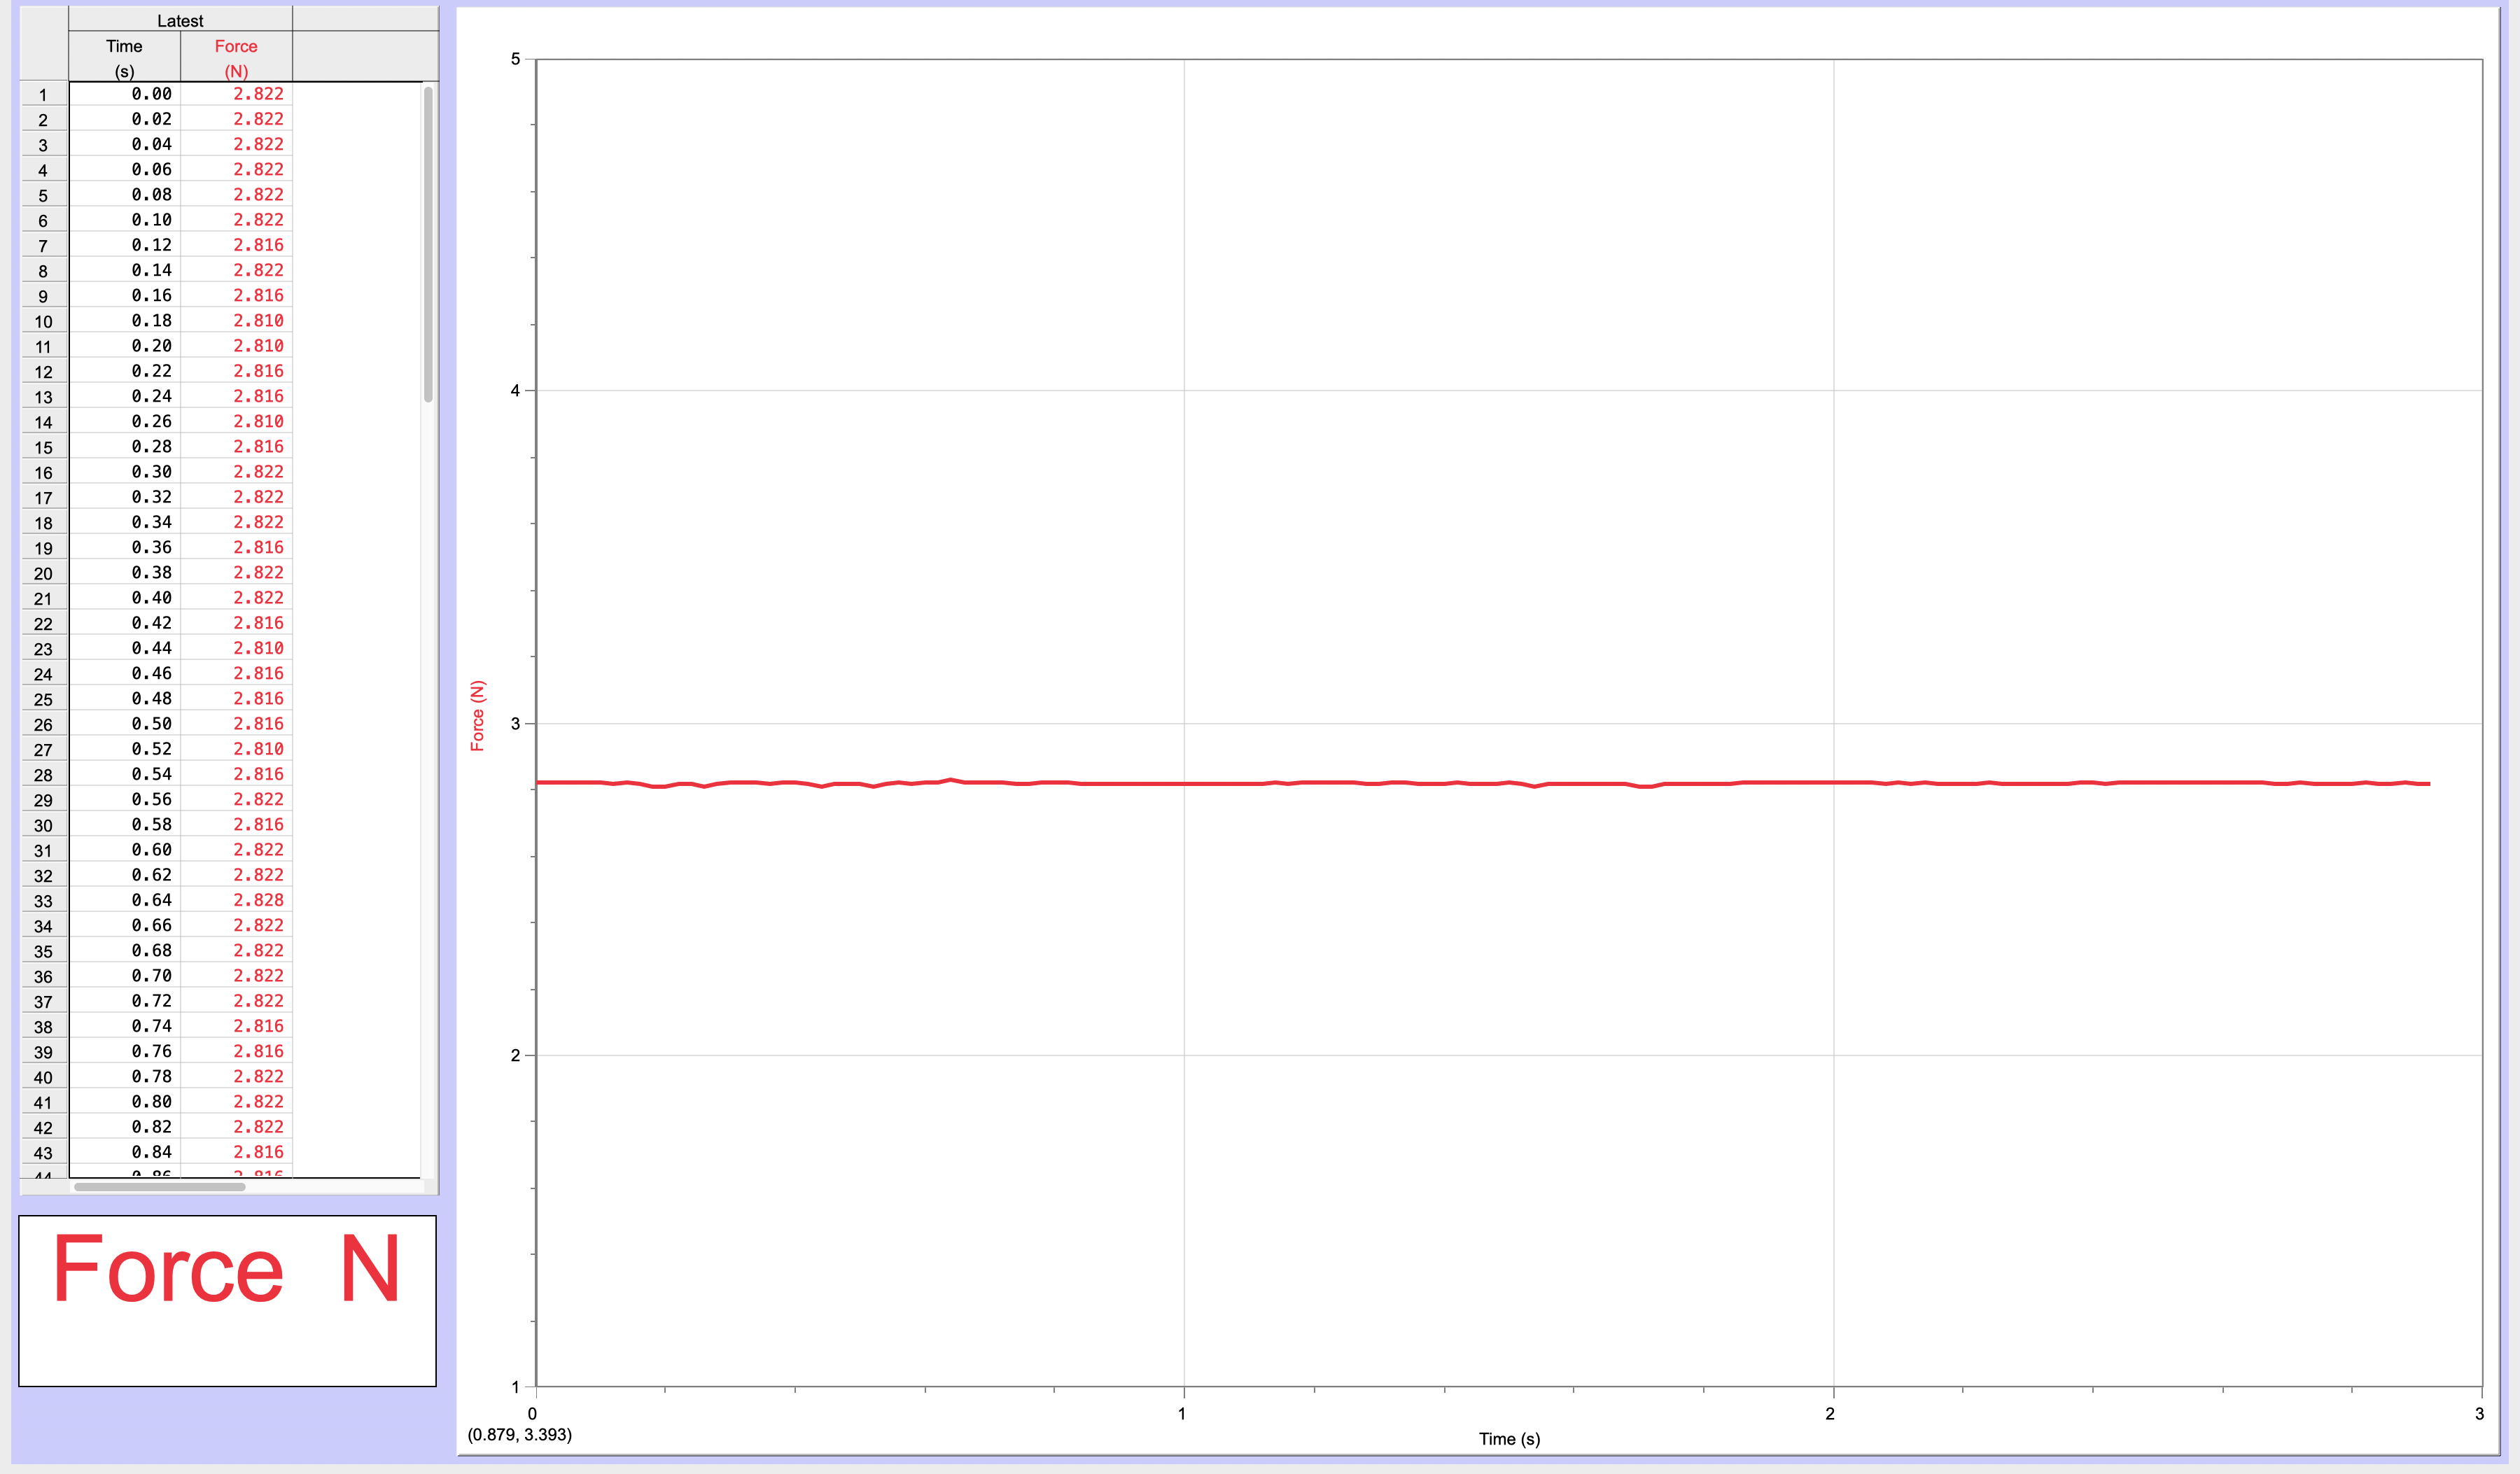
\includegraphics[width=.90\linewidth]{images/Lab.05/Lab05.Run4.png}
\end{center}
\caption{Run 4 of 6. This run, the force sensor was mounted on the stand \textbf{vertically} using the \textbf{thumb screw} and the \textbf{handle}. Using the \textbf{hook}, we attached \textbf{weights} to it (\textbf{285GM}) and measured a \textbf{constant force}.}
\label{fig:Lab05-Run4}
\end{figure}

\begin{figure}[H] % Example of including images
\begin{center}
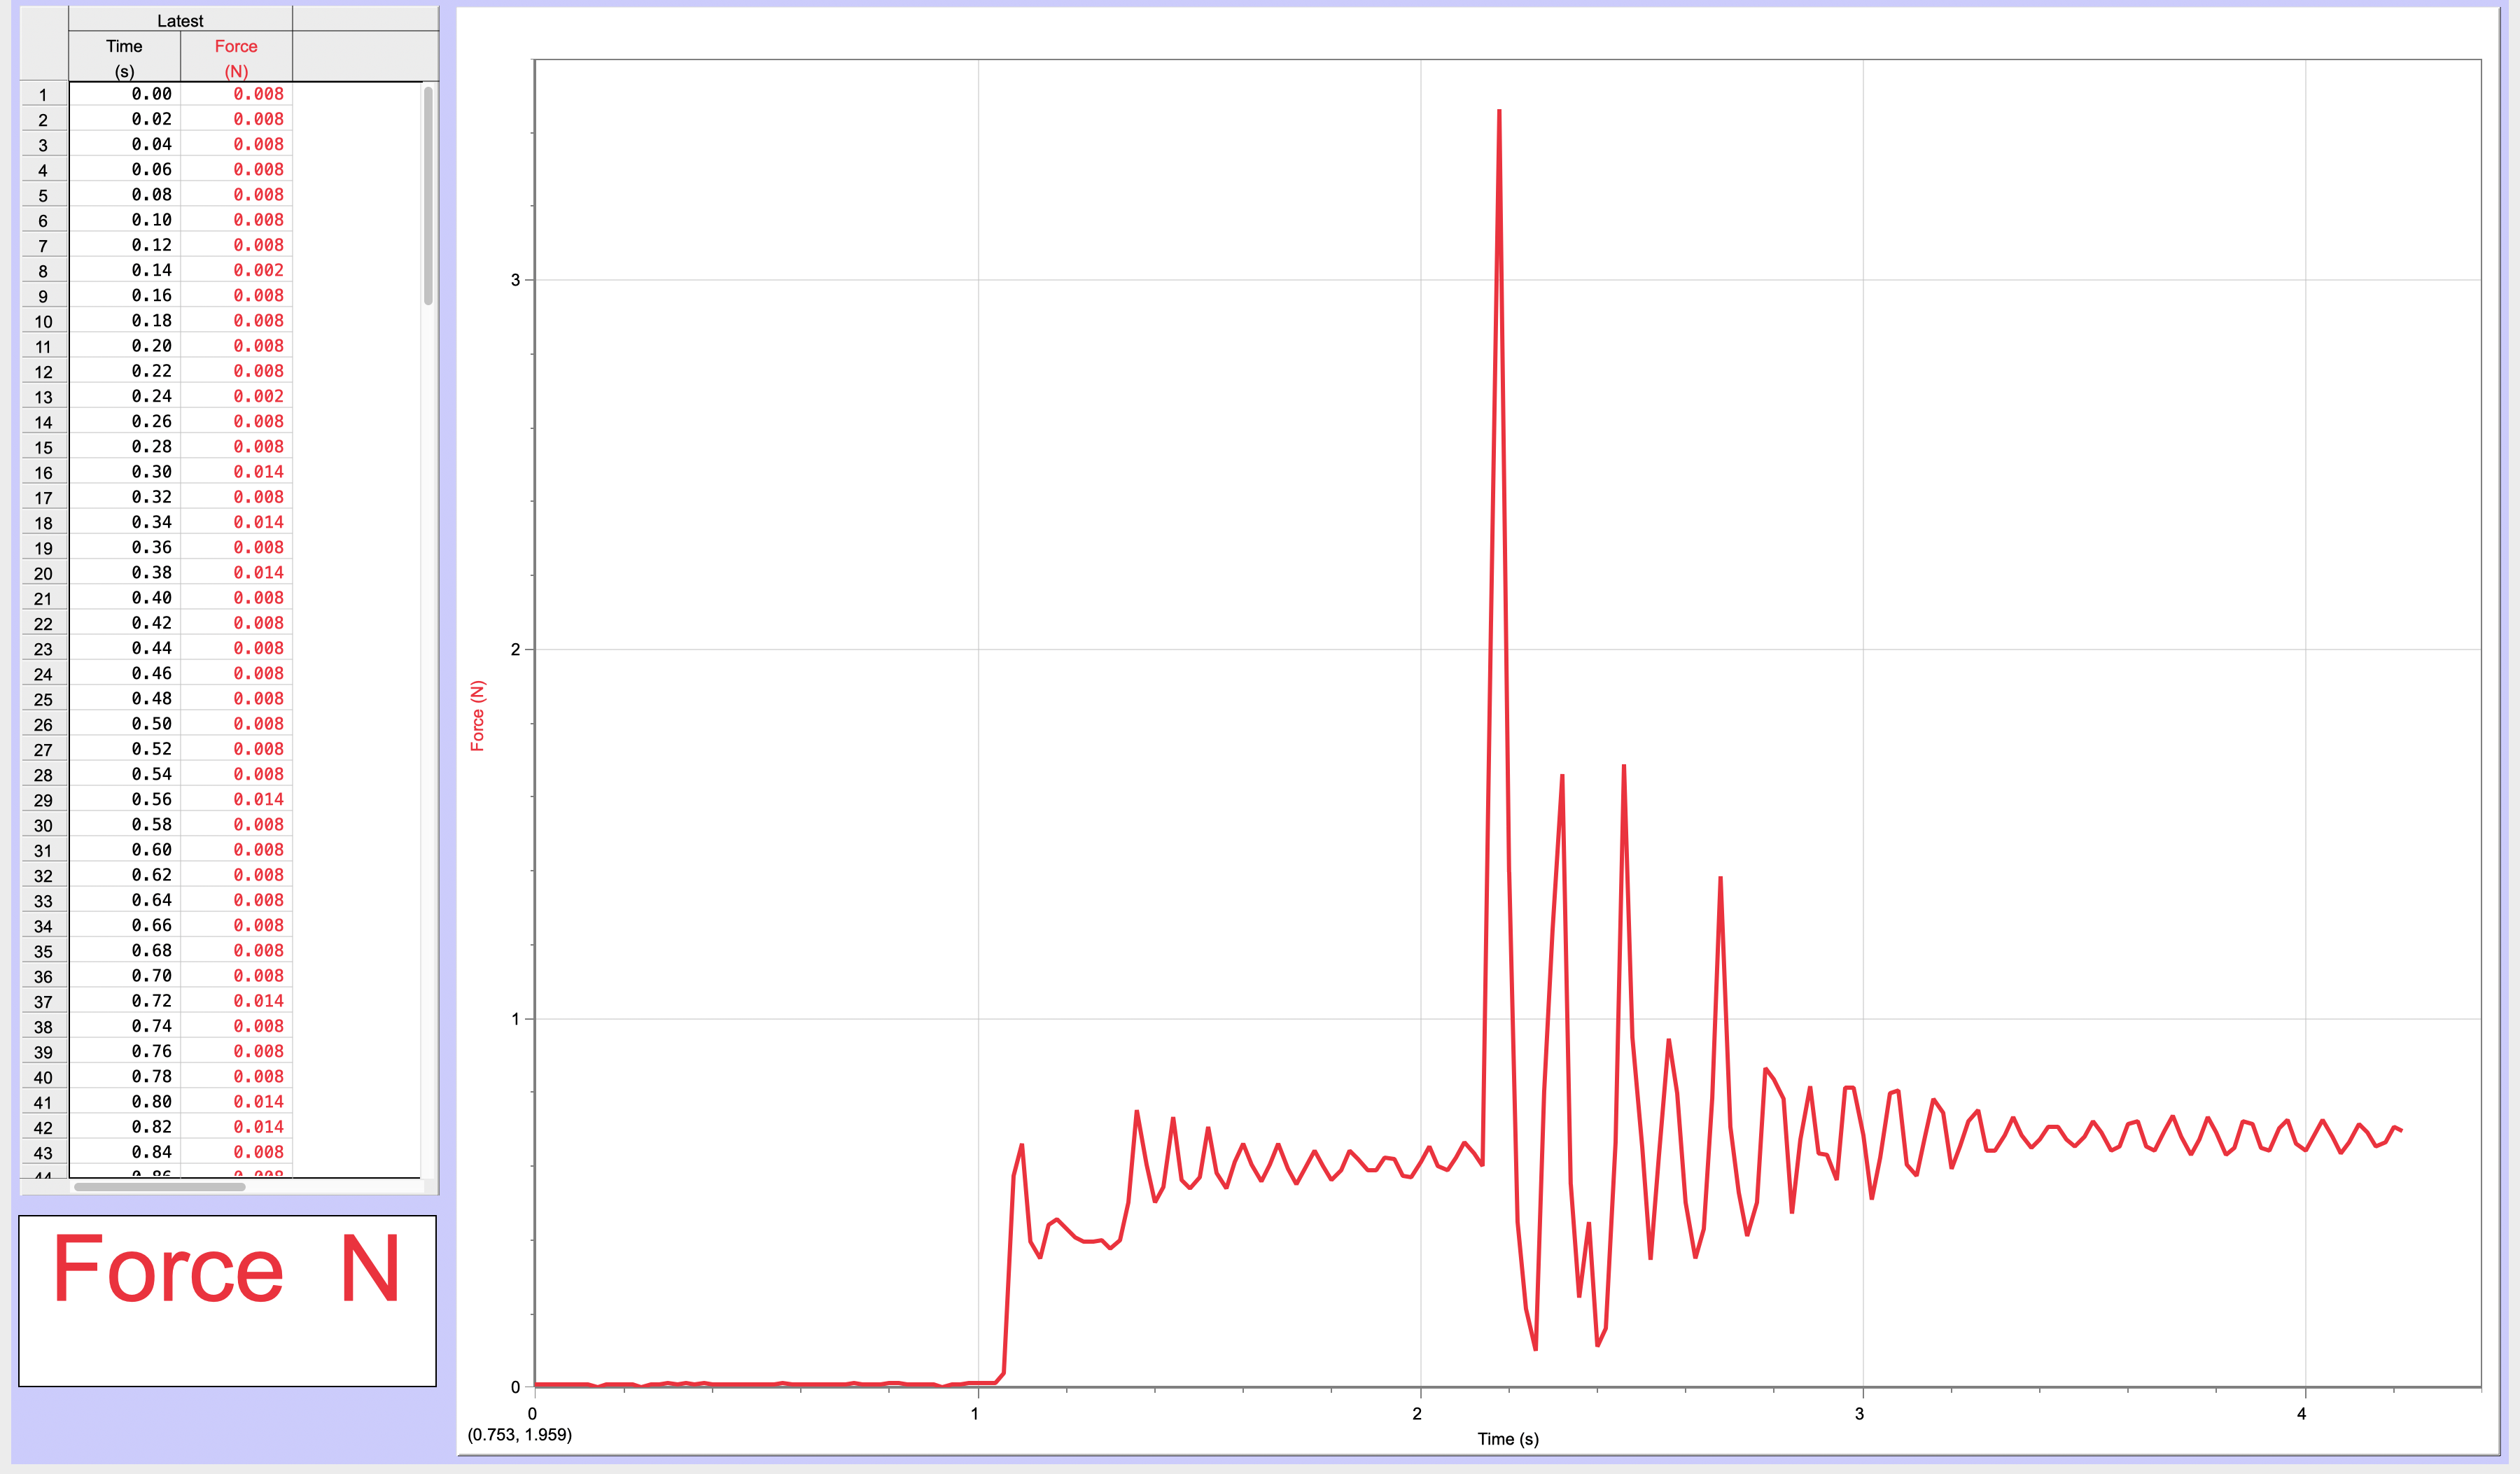
\includegraphics[width=.80\linewidth]{images/Lab.05/Lab05.Run5.png}
\end{center}
\caption{Run 5 of 6. This run, the force sensor was \textbf{vertically} mounted on the cart using the \textbf{thumb screw} and the \textbf{handle}. We also added the \textbf{bumper} to the force sensor and we then attached \textbf{weights} to it and ran it down along the \textbf{wheel}. The angle of the track we set it on was \textbf{2.20 degrees} and we attached \textbf{70GM} of \textbf{weights} to it, while measuring a \textbf{constant force, zero net force}.}
\label{fig:Lab05-Run5}
\end{figure}

\begin{figure}[H] % Example of including images
\begin{center}
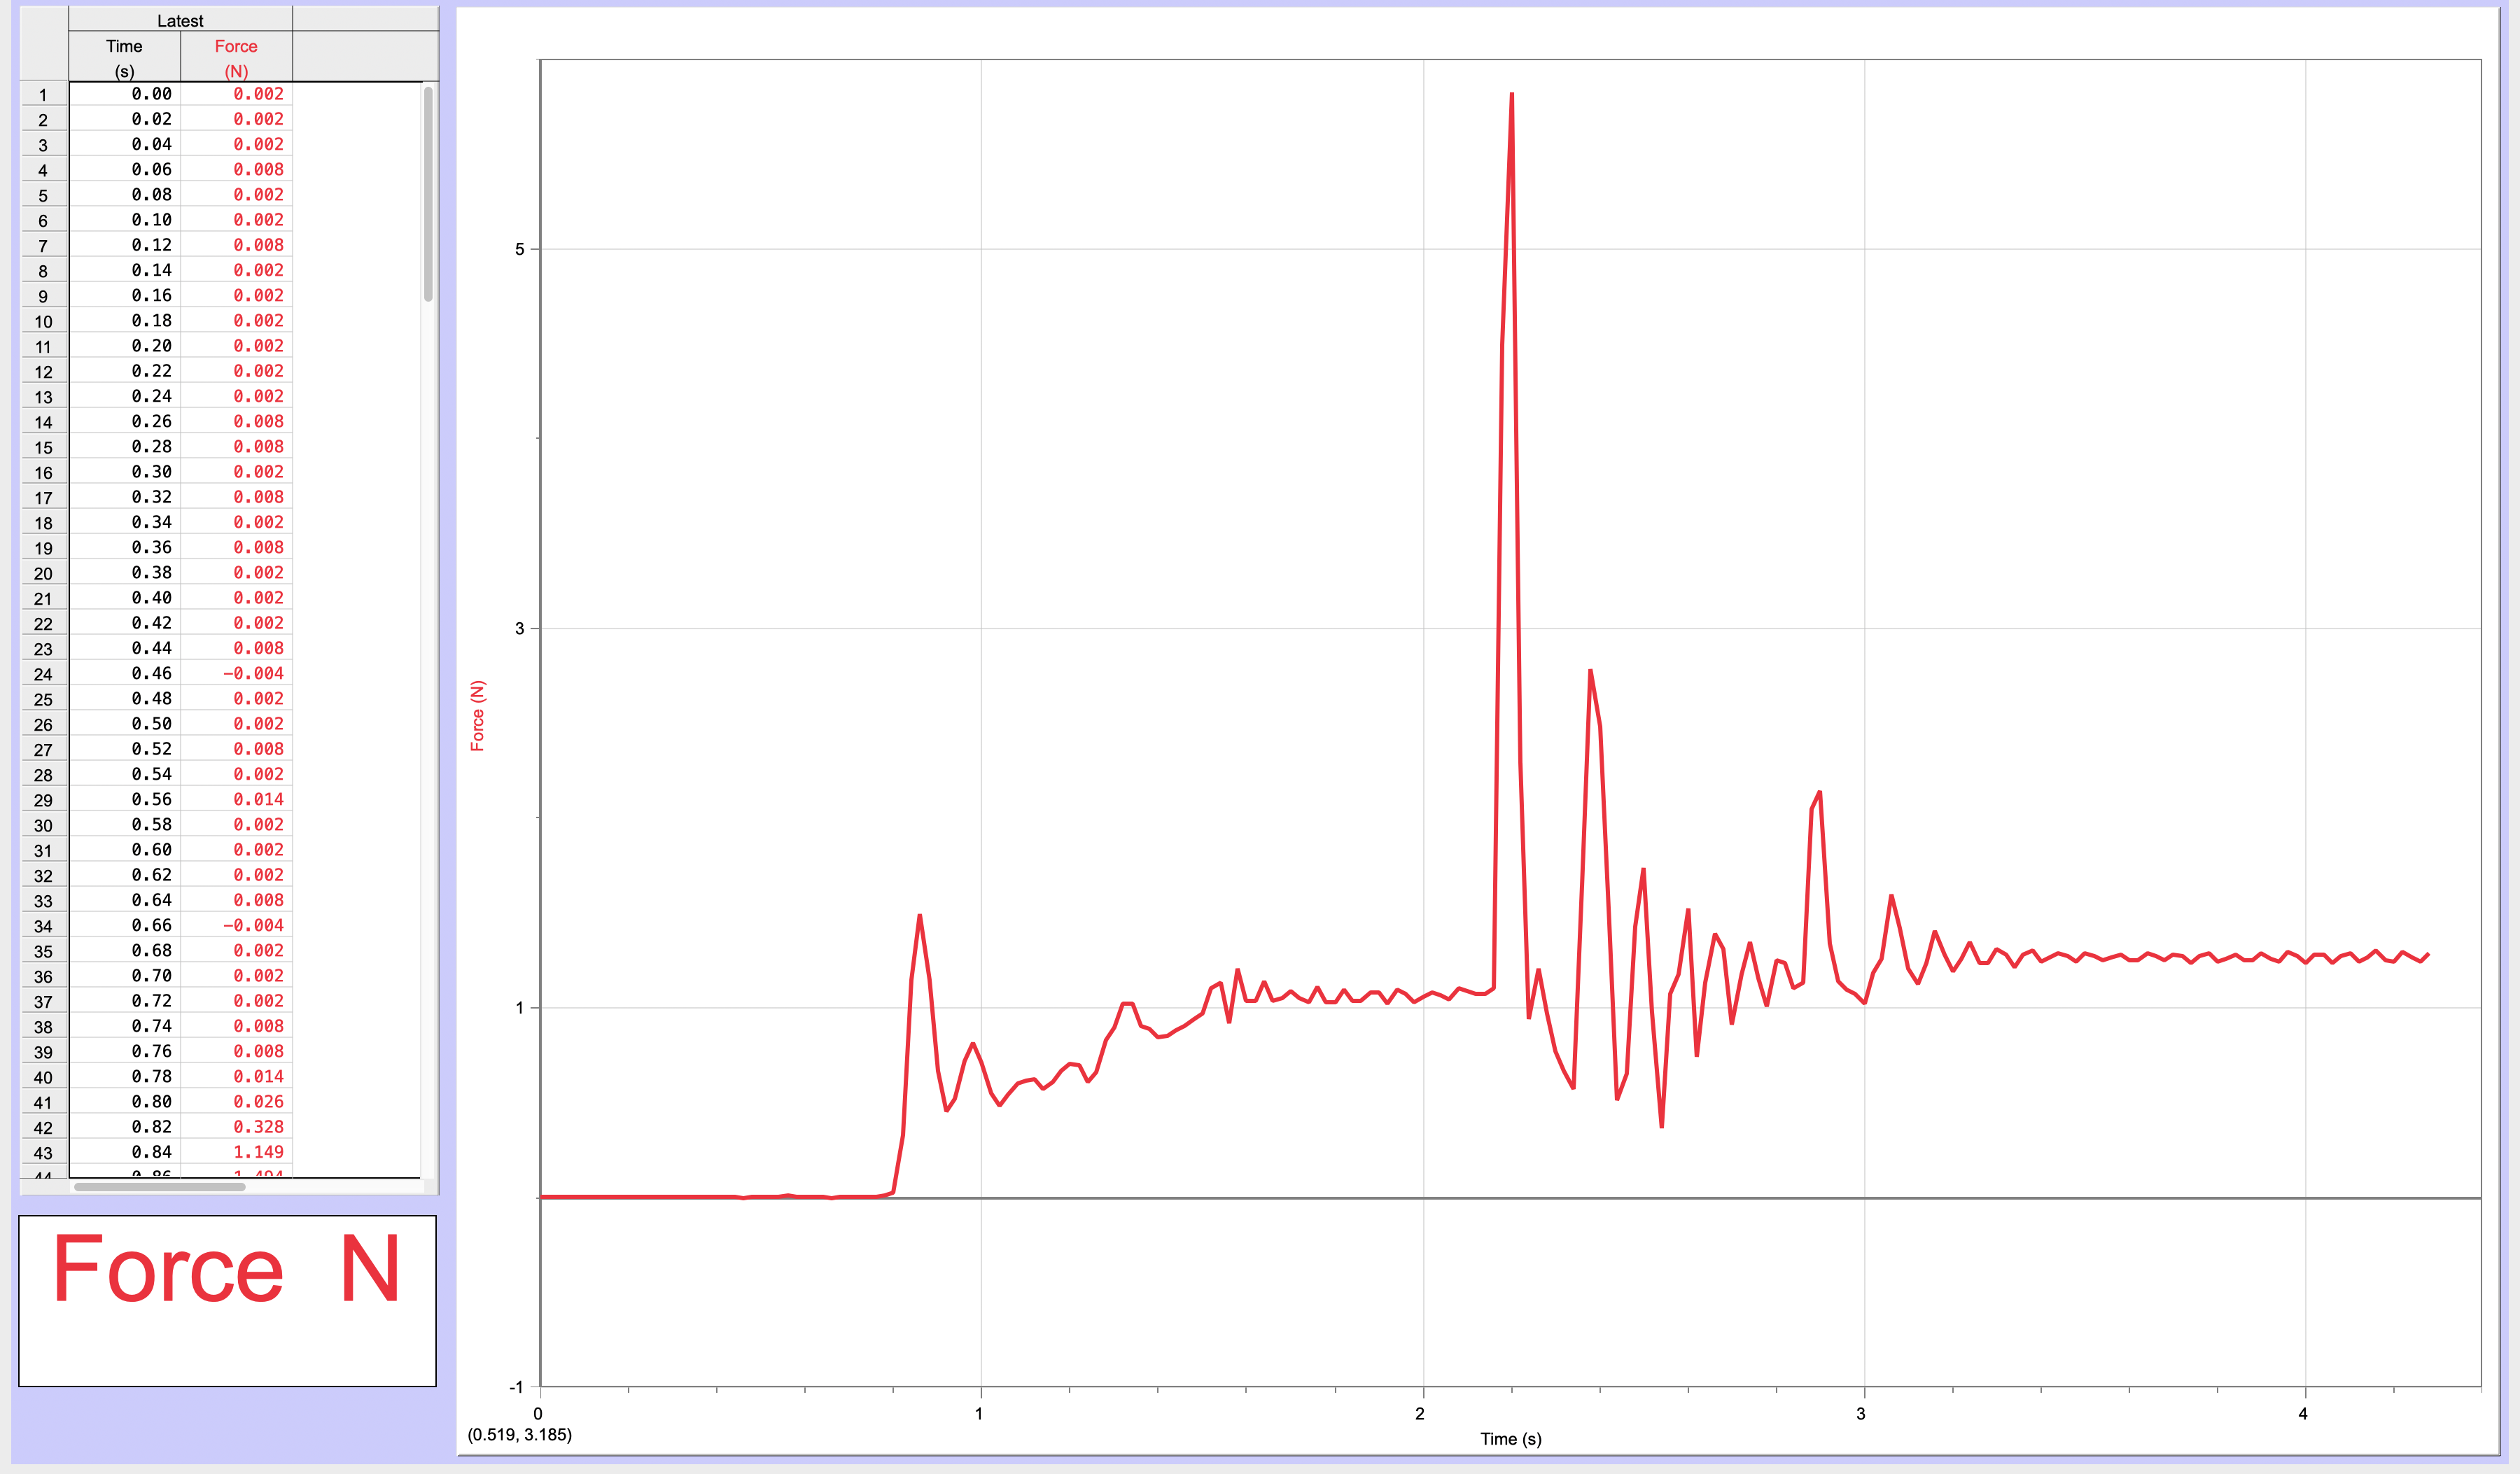
\includegraphics[width=.80\linewidth]{images/Lab.05/Lab05.Run6.png}
\end{center}
\caption{Run 6 of 6. This run, the force sensor was \textbf{vertically} mounted on the cart using the \textbf{thumb screw} and the \textbf{handle}. We also added the \textbf{bumper} to the force sensor and we then attached \textbf{weights} to it and ran it down along the \textbf{wheel}. The angle of the track we set it on was \textbf{8 degrees} and we attached \textbf{130GM} of \textbf{weights} to it, while measuring a \textbf{constant force, zero net force}.}
\label{fig:Lab05-Run6}
\end{figure}

%----------------------------------------------------------------------------------------

\experiment{Lab Notebook Prompts and Answers}
Required in your work: \textit{(This list is in no particular order, and you may incorporate different aspects into your measurements.)}
\begin{itemize}
    \item Orientations of the force sensor. \textbf{We mounted the force sensor both vertically and horizontally, see all figures above.}
    \begin{itemize}
        \item Vertical: mounted on the lab stand and holding it vertically. \textbf{See figures: \ref{fig:Lab05-Run3}, \ref{fig:Lab05-Run4}, \ref{fig:Lab05-Run5}, \ref{fig:Lab05-Run6}}
        \item Horizontal: mounted on the lab stand and laying on the table. \textbf{See figures: \ref{fig:Lab05-Run2}}
        \item On the cart track at different angles. \textbf{See figures: \ref{fig:Lab05-Run2}, \ref{fig:Lab05-Run5}, \ref{fig:Lab05-Run6}}
    \end{itemize}
    \item Force sensor attachments:
    \begin{itemize}
        \item Hook. \textbf{See figures: \ref{fig:Lab05-Run2}, \ref{fig:Lab05-Run3}, \ref{fig:Lab05-Run4}}
        \item Bumper. \textbf{See figures: \ref{fig:Lab05-Run5}, \ref{fig:Lab05-Run6}}
        \item Sensor mounted on lab stand (thumb screw to secure). \textbf{See all figures above.}
        \item Handle. \textbf{See figures: \ref{fig:Lab05-Run3}, \ref{fig:Lab05-Run4}, \ref{fig:Lab05-Run5}, \ref{fig:Lab05-Run6}}
    \end{itemize}
    \item You must explore different types of forces. \textbf{See all figures above.}
    \item Force conditions. \textbf{See all figures above.}
    \begin{itemize}
        \item Constant, non-zero forces. \textbf{See figures: \ref{fig:Lab05-Run2}}
        \item Constant, zero net force. \textbf{See figures: \ref{fig:Lab05-Run5}, \ref{fig:Lab05-Run6}}
        \item Non-constant forces. \textbf{See figures: \ref{fig:Lab05-Run3}, \ref{fig:Lab05-Run4}}
    \end{itemize}
    \item Compare weights from mass balances and force sensors. \textbf{The sensor and balance were similar weights, they both weighed correctly.}
\end{itemize}

%----------------------------------------------------------------------------------------

\labday{Wednesday, 20 March 2024}
\vspace{-5mm}
Tiffany Pham

\experiment{Lab 06 (Lab) - Friction}
\textbf{Purpose}
\begin{enumerate}
    \item Use your lab notebook to document your work and reasoning; referring to the lab notebook guidelines as needed.
    \item Correctly zero the Vernier dual-range force sensor.
    \item Measure forces using the Vernier dual-range force sensor.
    \item Determine which sensor attachments to use and ranges to use for accurate, reproducible force measurements in various ways with the provided materials.
\end{enumerate}

\hfill \break
\textbf{Objective}

Use the force sensor to determine the static and kinetic friction coefficients for a variety
of materials in the lab.

\hfill \break
\textbf{Predictions}

I predict that the force sensor will be able to somewhat accurately measure the kinetic and static friction with a +-2 deviation.

\hfill \break
\textbf{Procedure}
\begin{enumerate}
    \item Turn on the computer or laptop and go to the Logger Pro application.
    \item Set up the track, cart, and force sensor alongside all the other needed attachments if it isn't set up already.
    \item Choose from one of the multiple surfaces to use from (sandpaper, bubble wrap, foil, felt, etc).
    \item Attach the friction sensor to the string and drag it along the surfaces. If it is not dragging, then add some weights as needed.
    \item Once you're done with a surface, then switch out the surfaces and repeat the steps.
\end{enumerate}

\hfill \break
What could go wrong:
\begin{itemize}
    \item The force sensor having false readings
\end{itemize}

\hfill \break
\textbf{Equipment needed}
\begin{itemize}
    \item Computer/ Laptop
    \item Logger Pro
    \item Vernier
    \item Force sensor
    \item Track
    \item Cart
    \item Attachments (hook, bumper, thumb screw, handle
    \item Forces (weights, string, etc)
    \item Surfaces (sandpaper, foil, felt, etc).
\end{itemize}

%----------------------------------------------------------------------------------------

\newpage
\experiment{Force Data}
\begin{figure}[H] % Example of including images
\begin{center}
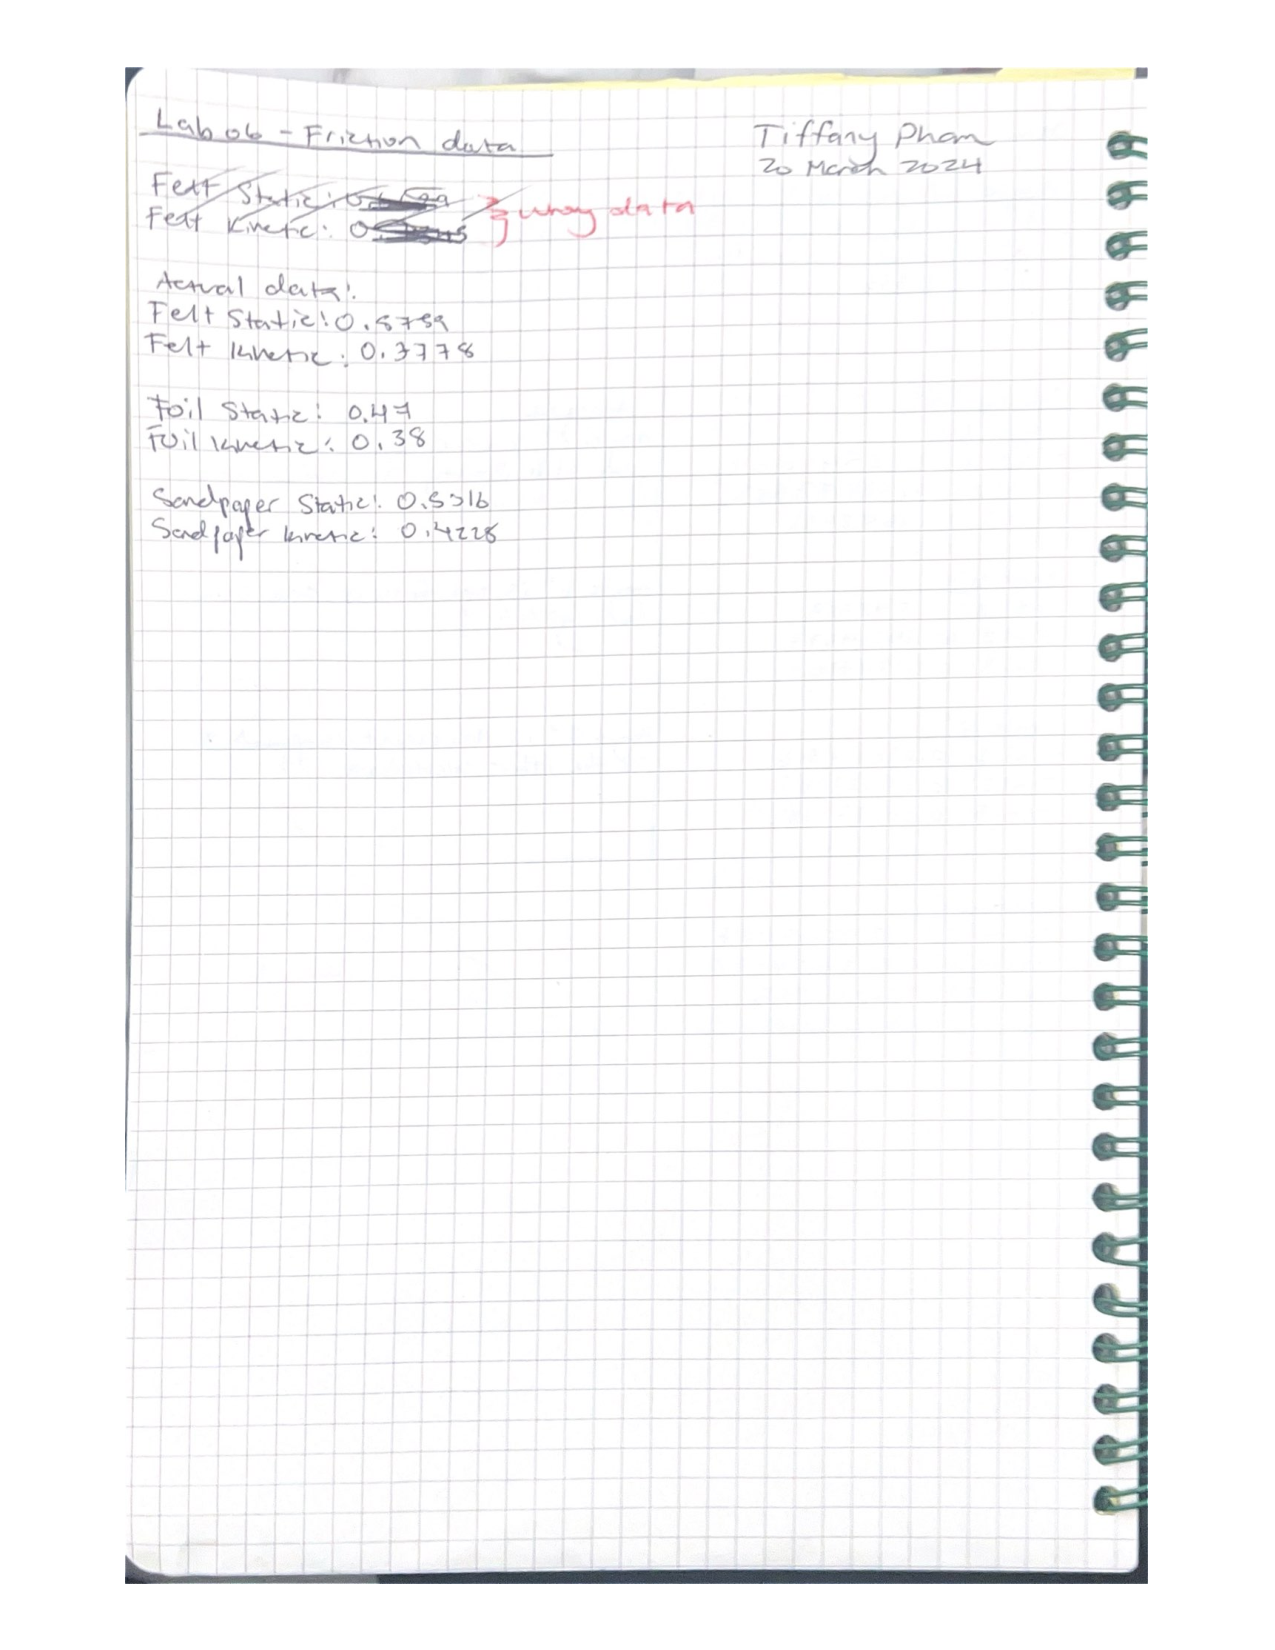
\includegraphics[width=0.8\linewidth]{images/Lab.06/Lab06Data.pdf}
\end{center}
\caption{This is the data from all the surfaces for the static and kinetic friction.}
\label{fig:Lab06Data}
\end{figure}

%----------------------------------------------------------------------------------------

\experiment{Lab Notebook Prompts}
\begin{enumerate}
    \item Use the force sensor to determine the static and kinetic friction coefficients for a variety of materials in the lab. How you do this is up to you and verify that your results are repeatable.
    \item For at least one combination of surfaces, and starting from rest, increase the applied force so that you see the changes in static friction, the transition, to motion, and the kinetic friction. Is your data reproducible?
    \item Compare your friction coefficients with your classmates’ values. (Think back to using the phyphox app to measure track incline angles.) Use this comparison to comment on different ways to find the friction coefficients.
\end{enumerate}

%----------------------------------------------------------------------------------------

\experiment{Lab Notebook Answers}
\begin{enumerate}
    \item I used multiple materials to measure such as the felt, foil, and sandpaper. The measurements are seen above in the figure.
    \item Yes, the data is reproducible.
    \item My data is similar to my classmates.
\end{enumerate}

% \begin{tabular}{l l l l l l l l l l l l l}
% \toprule
% \textbf{Name} & \textbf{Track 1} & \textbf{Track 2} & \textbf{Track 3} & \textbf{Track 4} & \textbf{Track 5} & \textbf{Track 6} & \textbf{Track 7} & \textbf{Track 8} & \textbf{Track 9} & \textbf{Track 10} & \textbf{Track 11} & \textbf{Track 12}    \\
% \toprule
% 1 & 0.2 & 0.8\\
% 2 & 0.17 & 0.7\\
% 3 & 0.24 & 0.75\\
% 4 & 0.68 & 0.3\\
% \bottomrule
% \end{tabular}
% \caption{The effects of treatments X and Y on the four groups studied.}
% \label{tab:treatments_xy}
% \end{table}


%----------------------------------------------------------------------------------------

% \labday{Saturday, Date Month Year}

% \experiment{Bulleted list example} % You don't need to make a \newexperiment if you only plan on referencing it once

% This is a bulleted list:

% \begin{itemize}
% \item Item 1
% \item Item 2
% \item \ldots and so on
% \end{itemize}

% %-----------------------------------------

% \experiment{example}

% \lipsum[6]

% %-----------------------------------------

% \experiment{example2}

% \lipsum[7]

% %----------------------------------------------------------------------------------------
% %	FORMULAE AND MEDIA RECIPES
% %----------------------------------------------------------------------------------------

% \labday{} % We don't want a date here so we make the labday blank

% \begin{center}
% \HRule \\[0.4cm]
% {\huge \textbf{Formulae and Media Recipes}}\\[0.4cm] % Heading
% \HRule \\[1.5cm]
% \end{center}

% %----------------------------------------------------------------------------------------
% %	MEDIA RECIPES
% %----------------------------------------------------------------------------------------

% \newpage

% \huge \textbf{Media} \\ \\

% \normalsize \textbf{Media 1}\\
% \begin{table}[H]
% \begin{tabular}{l l l}
% \toprule
% \textbf{Compound} & \textbf{1L} & \textbf{0.5L}\\
% \toprule
% Compound 1 & 10g & 5g\\
% Compound 2 & 20g & 10g\\
% \bottomrule
% \end{tabular}
% \caption{Ingredients in Media 1.}
% \label{tab:med1}
% \end{table}

% %-----------------------------------------

% %\textbf{Media 2}\\ \\

% %Description

% %----------------------------------------------------------------------------------------
% %	FORMULAE
% %----------------------------------------------------------------------------------------

% \newpage

% \huge \textbf{Formulae} \\ \\

% \normalsize \textbf{Formula 1 - Pythagorean theorem}\\ \\
% $a^2 + b^2 = c^2$\\ \\

%-----------------------------------------

%\textbf{Formula X - Description}\\ \\

%Formula

%----------------------------------------------------------------------------------------

\end{document}